\documentclass[11pt,a4paper]{article}


\usepackage[margin = 1in]{geometry}
\usepackage{amsfonts,amssymb,amsmath}
\usepackage{graphicx}
\usepackage[none]{hyphenat}
\usepackage{float}
\usepackage{fancyhdr}
\usepackage{color}
\usepackage{tikz}
\usepackage[nottoc,notlot,notlof]{tocbibind}


\parindent 0ex





\usetikzlibrary{quotes,angles,arrows.meta,fadings,shapes,trees,bending,patterns}





% Theorem environments. The source declared none, so every result was set as
% bold text: unnumbered, unreferenceable, and invisible to the site's styling.
% Names match the other courses here so a block of text moves between them.
\usepackage{amsthm}
\theoremstyle{definition}
\newtheorem{thm}{Theorem}[section]
\newtheorem{defn}[thm]{Definition}
\newtheorem{exa}[thm]{Example}
\newtheorem{note}[thm]{Note}
\newtheorem{remark}[thm]{Remark}
\newtheorem{prop}[thm]{Proposition}
\newtheorem{coro}[thm]{Corollary}
\newtheorem{lem}[thm]{Lemma}
\newtheorem{result}[thm]{Result}
% Practice problems, numbered separately so adding one never renumbers a
% theorem the text refers to.
\newtheorem{problemx}{Problem}[section]
\newenvironment{problem}{\begin{problemx}}{\end{problemx}}
\newenvironment{solution}
  {\renewcommand{\qedsymbol}{}\begin{proof}[\textit{Solution}.]}
  {\end{proof}}
% enumitem: without it tex4ht discards the optional \item[(a)] labels.
\usepackage{enumitem}

\begin{document}




% Title page depersonalised for the web, as with every other course here: no
% university, no lecturer, no author, no year. The original named a third
% party as lecturer, which is not ours to publish. The identity kept below is
% the multivariate normal density, which is what the course is about.
\begin{titlepage}
\begin{center}
\vspace*{3cm}
{\Huge\bfseries Multivariate Statistical Analysis}\\[1.2cm]
{\large Lecture Notes}\\[2.5cm]
\line(1,0){300}\\[1.5cm]
$$f(\mathbf{x}) = \frac{1}{(2\pi)^{p/2}\left|\Sigma\right|^{1/2}}
\exp\left\{-\tfrac{1}{2}(\mathbf{x}-\boldsymbol{\mu})'\,\Sigma^{-1}
(\mathbf{x}-\boldsymbol{\mu})\right\}$$
\end{center}
\end{titlepage}



\pagestyle{fancy}
\fancyhead{}
\fancyfoot{}
\fancyhead[R]{\rightmark\qquad  \thepage}
\renewcommand{\headrulewidth}{0pt}


\textcolor{blue}\tableofcontents
\thispagestyle{empty}
\clearpage
\setcounter{page}{1}





%\chapter{\textcolor{red}{MATRIX ALGEBRA}}
\section{Review of Matrix Algebra}
\subsection{Matrix}
We define a matrix \begin{equation}\tag{1}
A = (a_{ij}) = 
\begin{pmatrix}
a_{11} & a_{12} & \cdots& a_{1p}\\
       & a_{22} & \cdots& a_{2p}\\
\vdots & \vdots &                    & \vdots\\
\vdots & \vdots &                    & \vdots\\
a_{n1} & a_{n2} & \cdots& a_{np}\\           
\end{pmatrix}
\end{equation}
as an $n\times p$ matrix of either constants or random variables.\\

Its transpose is denoted by $$A' = A^T = (a_{ij})_{ji}\qquad i = 1,2,\ldots,n\qquad j=1,2,\ldots,p$$\\



\begin{note}
\begin{enumerate}
\item If the entries of $A$ are constants then $A$ is a constant matrix.
\item If the entries of $A$ are random variables then $A$ is said to be a random matrix.\\\\
\end{enumerate}
\end{note}
















\subsection{Vector}
A matrix with column order is called  a column vector
\begin{equation}\tag{2}
\underline{a} = 
\begin{pmatrix}
a_1\\
a_2\\
\vdots\\
\vdots\\
a_n\\
\end{pmatrix}
\end{equation}
its transponse $\underline{a}'=
\begin{pmatrix}
a_1, & a_2, \ldots, & a_n\\
\end{pmatrix}$ is a row vector.\\

Again 
\begin{enumerate}
\item If the entries are constants then the vector is constant vector.
\item If the entries are random variables then the vector is a random vector.\\
\end{enumerate}


It is possible to write a matrix in equation (1) as vector.\\
i.e $A = \begin{pmatrix}
\underline{a}_1, & \underline{a}_2, \ldots, & \underline{a}_p\\
\end{pmatrix}$ , where $\underline{a}_i$ is the $i^{\text{th}}$ column vector.\\\\\\





\pagebreak
\begin{exa}
Data on Incidence of poverty by province from 1991, 1993 and 1996.
\end{exa}


\begin{table}[H]
\centering
\begin{tabular}{|c|c|c|c|}
\hline
Province & 1991 & 1993 & 1996\\
\hline
Central & 55.7 & 70.7 & 58.6\\
Copperbelt & 43.8 & 28.1 & 33.5\\
Eastern & 76.1  & 81.2 & 69.9\\
Luapula & 72.5 & 77.8 & 63.9\\
Lusaka  & 18.7 & 24.3 & 22\\
Northern & 75.9  & 71.5 & 69.4\\
N Western & 64.5 & 75.5 & 64.8\\
Southern & 69.4 & 76.1 & 58.6\\
Western & 75.8 & 33.5 & 73.6\\
\hline
\end{tabular}
\caption{}
\end{table}



\begin{note}
\begin{enumerate}
\item In this Data set we have four variables, province, incidence of poverty 1991, 1993, 1996
\item Before data the was collected the incidence of poverty where unknown and the variables would be random variables. But after the data were collected we have observed values of random variables.
\item The columns represent vectors, the rows also vectors.\\\\
\end{enumerate}
\end{note}





$\bullet$ A matrix written in terms of its sub-matrices is called a partitioned matrix.\\

Let $A_{11}$, $A_{12}$ , $A_{21}$ and $A_{22}$ be sub-matrices of matrix $A$ such that $A_{r\times s}$ has elements $a_{ij},\\\qquad i=1,2,\ldots r\qquad j=1,2,\ldots,s$ then we write
$$A_{n\times p} =
\begin{pmatrix}
A_{r\times s} & A_{r\times (p-s)}\\
&\\
A_{(n-r)\times s} & A_{(n-r)\times (p-s)}\\
\end{pmatrix}
$$\\



\begin{exa}
\begin{enumerate}
\item If $B = 
\begin{pmatrix}
13 & -4 & 2\\
3 & 12 & 0\\
2 & -2 & 10\\
\end{pmatrix}
$ then one possible partition of $B$ could be

$$B_{11} =
\begin{pmatrix}
13 & -4\\
3 & 12\\
\end{pmatrix}_{2\times 2}, 
B_{12} = 
\begin{pmatrix}
2\\
0\\
\end{pmatrix}_{2\times 1}, 
B_{21} =
\begin{bmatrix}
2, & -2\\
\end{bmatrix}_{1\times 2}, 
B_{22} =
\begin{bmatrix}
10\\
\end{bmatrix}_{1\times 1}
$$

\item In the poverty data, let $A_{11}$ consists of 2 rows consisting of Lusaka and Copperbelt one column for 1991 data. i.e $B_{11}$ is $2\times 1$ matrix determine $B_{12}$ , $B_{21}$ and $B_{22}$.\\\\
\end{enumerate}
\end{exa}




\subsection{Some Particular Matrices}

\begin{table}[H]
\centering
\begin{tabular}{|c|ccc|}
\hline
Name & Definition & Notation & Trivial Example\\
\hline
Scalar & $p=n=1$ & $a,b$ & $(1)= 1$\\
&&&\\
Square & $p=n$ & $A_{p\times p}$ & $
\begin{pmatrix}
1 & 3\\
4 & 5\\
\end{pmatrix}_{2\times 2}
$\\
&&&\\
Diagonal & $p=n, a_{ij}=0, i\neq j$ & $Diag(a_{ij})$ & $
\begin{pmatrix}
2 & 0\\
0 & 4\\
\end{pmatrix}
$\\
&&&\\
Identity & $Diag(1)$ & $I$ or $I_p$ & $
\begin{pmatrix}
1 & 0\\
0 & 1\\
\end{pmatrix}
$\\
&&&\\
Symmetric & $a_{ij} = a_{ji}$ & & $
\begin{pmatrix}
1 & 2\\
2 & 1\\
\end{pmatrix}
$\\
&&&\\
Unit matrix & $p=n, a_{ij}=1$ & $J_p = \underline{1}\,\underline{1}'$ & $
\begin{pmatrix}
1 & 1\\
1 & 1\\
\end{pmatrix}
$\\
&&&\\
Triangular & $a_{ij} = 0$ & $\Delta$ & $\begin{pmatrix}
1 & 0 & 0\\
2 & 2 & 0\\
3 & 2 & 5\\
\end{pmatrix}
$\\
      & below/ above the & &\\
      &  diagonal &  &\\
Asymmetric & $a_{ij} \neq a_{ji}$ & & $\begin{pmatrix}
1 & 1\\
2 & 3\\
\end{pmatrix}$\\
&&&\\
Null & $a_{ij} =0$ & 0 & $\begin{pmatrix}
0 & 0 & 0 & 0\\
0 & 0 & 0 & 0\\
0 & 0 & 0 & 0\\
0 & 0 & 0 & 0\\
\end{pmatrix}$\\
\hline
\end{tabular}
\caption{}
\end{table}
\vspace{2cm}










\pagebreak
\subsection{Basic Matrix Operations}
We assume the usual matrix operations of addition, subtraction, scalar multiplication, inner product, multiplication, transpose, trace, determinant and inverse.\\

\begin{exa}

If $A = \begin{pmatrix}
1 & 3 & 2\\
-1 & 4 & 0\\
2 & 5 & 2\\
\end{pmatrix}$
\end{exa}


\begin{enumerate}
\item $\displaystyle{Tr(A) = \sum^3_{i=1}a_{ii} = a_{11} + a_{22} + a_{33} = 1 + 4 + 2 = 7}$

\item 
\begin{align*}
\det (A) & = |A| = 1 \begin{vmatrix}
4 & 0\\
5 & 2\\
\end{vmatrix} - (-1)
\begin{vmatrix}
3 & 2\\
5 & 2\\
\end{vmatrix} + 2 \begin{vmatrix}
3 & 2\\
4 & 0\\
\end{vmatrix}\\\\
& = (8-0) + (6-10) + 2(0-8)\\
& = 8 - 4 - 16\\
& = -12\\
\end{align*}

\item\quad 
$\displaystyle{
B = A + A'  = \begin{pmatrix}
1 & 3 & 2\\
-1& 4 & 0\\
2 & 5 & 2\\
\end{pmatrix} + \begin{pmatrix}
1 & -1 & 2\\
3 & 4 &  5\\
2 & 0 & 0\\
\end{pmatrix}
 = \begin{pmatrix}
2 & 2 & -4\\
2 & 8 & 5\\
4 & 5 & 4\\
 \end{pmatrix}
= B'}$

\begin{note}
\begin{enumerate}
\item $B = (b_{ij})$
\item $B' = (b_{ji})$
\item $B = B'$\\\\
\end{enumerate}
\end{note}
\end{enumerate}



\subsubsection{The Trace Function}

The trace function satisfies the following properties:
$$A_{p\times p},  B_{p\times p},  C_{p\times n},  D_{n\times p}\qquad\text{and scalar}\quad  \alpha$$

\begin{enumerate}
\item $Trace(\alpha) = \alpha$

\item $Tr(A\pm B) = Tr(A) \pm Tr(B)$

\item $Tr(\alpha A) = \alpha Tr(A)$

\item $Tr(CD) = Tr(DC) = \displaystyle{\sum c_{ij}d_{ji}}$\\\\
\end{enumerate}




\pagebreak


\subsubsection{Square Matrix}

A square matrix is non-singular if $|A| \neq 0$ , otherwise it is singular.\\

The following results follow
\begin{enumerate}
\item $|A|= \displaystyle{\sum^p_{j=1}a_{ij}A_{ij}}$, where $A_{ij}$ is the determinant of the cofactor $\displaystyle{A_{ij}=(-1)^{i+j}|A_{ij}|}$.

\item If $A$ is triangular or diagonal then $\displaystyle{|A| = \prod^p_{i=1} a_{ii}}$.

\item $\displaystyle{|\alpha A| = \alpha^p |A|}$

\item $\displaystyle{|AB| = |A||B|}$

\item For square sub-matrices $A_{p\times p}$ and $B_{q\times q}$
$$
\begin{vmatrix}
A & C\\
0 & B\\
\end{vmatrix} = \begin{vmatrix}
A\\
\end{vmatrix}\begin{vmatrix}
B\\
\end{vmatrix}
$$

$$A^* =
\begin{pmatrix}
A & C\\
0 & B\\
\end{pmatrix}_{(p + q)\times (p + q)}
$$


\item $\displaystyle{
\begin{vmatrix}
A_{11} & A_{12}\\
A_{21} & A_{22}\\
\end{vmatrix}=\begin{vmatrix}
A_{11}\\
\end{vmatrix}\begin{vmatrix}
A_{22} - A_{21}A^{-1}_{11}A_{12}\\
\end{vmatrix}
}$ for square $A_{11}$ and $A_{22}$.\\\\




\begin{proof}
Assume $A^{-1}_{11}$ exists $   
\begin{pmatrix}
A_{11} & A_{12}\\
\end{pmatrix}
$. Pre-multiply ``row 1" by $A_{21}A^{-1}_{11}$ and subtract from\\ ``row 2"
\end{proof}


\begin{align*}
\begin{vmatrix}
A_{11} & A_{12}\\
A_{21}-A_{21}A_{11}^{-1}A_{11} & A_{22}-A_{21}A^{-1}_{11}A_{12}\\
\end{vmatrix} & =
\begin{vmatrix}
A_{11} & A_{12}\\
0 & A_{22} - A_{21}A_{11}^{-1}A_{12}\\
\end{vmatrix}\\\\
& = \begin{vmatrix}
A_{11}\\
\end{vmatrix}\begin{vmatrix}
A_{22} -A_{21}A_{11}^{-1}A_{12}\\
\end{vmatrix}\qquad\text{using result (5)}\\\\
\end{align*}
\end{enumerate}


\pagebreak




\subsection{Further Matrices}

\begin{table}[H]
\centering
Particular Type Of Matrices\\
\begin{tabular}{|c|c|c|}
\hline
Name & Definition & Example\\
\hline
&&\\
Non-Singular & $\begin{vmatrix}
A\\
\end{vmatrix}\neq 0$ & $\begin{bmatrix}
1 & 2\\
0 & 1\\
\end{bmatrix}$, $\quad \begin{vmatrix}
A\\
\end{vmatrix} =1$\\
&&\\
\hline
&&\\
Singular & $\begin{vmatrix}
A\\
\end{vmatrix} = 0$ & $\begin{bmatrix}
1 & 2\\
1 & 2\\
\end{bmatrix}$ $, \begin{vmatrix}
A\\
\end{vmatrix}=0$\\
&&\\
\hline
&&\\
Orthogonal & $A'A = AA' =I$ & $\begin{bmatrix}
\cos \theta & -\sin \theta\\
\sin \theta & \cos \theta\\
\end{bmatrix}$\\
&&\\
\hline
&&\\
Idempotent & $A^2 =A$ & $\frac{1}{2}\begin{bmatrix}
1 & -1\\
-1 & 1\\
\end{bmatrix}$\\
&&\\
\hline
&&\\
Centering & $H_n = I_n - n^{-1}J_n$ & \\
&&\\
\hline
&&\\
Positive Definite (p.d) & $X'AX>0$ for & $x^2_1 + x_2^2$\\
                        & all $\underline{X}\neq \underline{0}$ & \\
&&\\
\hline
&&\\
Positive & $\underline{X}'A\underline{X}\geq 0$ & $(x_1-x_2)^2$\\
Semi-definite (p.s.d) & $\forall \underline{X}\neq 0$ &  \\
\hline
\end{tabular}
\caption{}
\end{table}



\vspace{0.5cm}

\textbf{Verification}
\begin{enumerate}
\item Idempotency\\

$\displaystyle{A^2 = A\quad :\qquad  A= \frac{1}{2}
\begin{bmatrix}
1 & -1\\
-1 & 1\\
\end{bmatrix}
}$

\begin{align*}
A^2 & = \Bigg(\frac{1}{2}\begin{bmatrix}
1 & -1\\
-1 & 1\\
\end{bmatrix}\Bigg) \Bigg(\frac{1}{2}\begin{bmatrix}
1 & -1\\
-1 & 1\\
\end{bmatrix}\Bigg)\\\\
& = \frac{1}{4}\begin{bmatrix}
1 & -1 \\
-1 & 1\\
\end{bmatrix}\begin{bmatrix}
1 & -1\\
-1 & 1\\
\end{bmatrix}=\frac{1}{4}\begin{bmatrix}
2 & -2\\
-2 & 2\\
\end{bmatrix}\\\\
& = \frac{2}{4}\begin{bmatrix}
1 & -1 \\
-1 & 1\\
\end{bmatrix}=
\frac{1}{2}\begin{bmatrix}
1 & -1\\
-1 & 1 \\
\end{bmatrix}=A\\
\end{align*}


\item $\underline{X}'A\underline{X}$\\

Let $y= A\underline{X}$, then $A$ is matrix of transformation.  $$y_i = \sum^p_{j=1} a_{ij}x_j$$
\begin{align*}
\underline{x}'\underline{y} & = \underline{x}\cdot \underline{y}\qquad\text{dot product}\\\\
& = \begin{vmatrix}
\underline{x}\\
\end{vmatrix}\begin{vmatrix}
\underline{y}\\
\end{vmatrix}\cos \alpha\qquad \text{where}\,\alpha\qquad\text{is the angle of ratation due to transformation}\\
\end{align*}

\begin{align*}
2.1\qquad  x^2_1 + x_2^2 & = 
\begin{pmatrix}
x_1 & x_2\\
\end{pmatrix}\begin{pmatrix}
x_1 \\
x_2\
\end{pmatrix}\qquad 
A= 
\begin{pmatrix}
1 & 0\\
0 & 1\\
\end{pmatrix}\\
& = \underline{X}'\underline{X}\\
& = \underline{X}'\begin{pmatrix}
1  & 0\\
0 & 1\\
\end{pmatrix}\underline{X}\\
& = \underline{X}' I_2 \underline{X}\\
& > 0\qquad\text{as long as any of} \, x_1,x_2\neq 0\\
& \implies\quad  \underline{X}\neq \underline{0}\\
\end{align*}


\begin{align*}
2.2\qquad  (x_1-x_2)^2 & = x_1^2 - 2x_1x_2 + x^2_2\\
& = (x_1 -x_2)(x_1-x_2)\\
& = \begin{pmatrix}
x_1 & x_2\\
\end{pmatrix}
\begin{pmatrix}
1 & -1 \\
-1 & 1\\
\end{pmatrix}\begin{pmatrix}
x_1\\
x_2\\
\end{pmatrix}\\
& = \begin{pmatrix}
x_1-x_2 & -x_1 + x_2\\
\end{pmatrix}\begin{pmatrix}
x_1\\
x_2\\
\end{pmatrix}\\
& = x^2_1 - x_1x_2 -x_1x_2 + x^2_2\\
\end{align*}




% DIAGRAM 1
\begin{figure}[H]
\centering
\begin{tikzpicture}[=>stealth]
\draw(-2,0)--(2,0)node[right]{$x_1$};
\draw(0,-2)--(0,2)node[above]{$x_2$};
\draw[smooth,domain=-2:2,thick, teal,variable=\x]plot({\x},{\x});
\draw(2,2)node[right]{$\underline{x}=\left(\begin{smallmatrix}
x_1\\
x_2\\
\end{smallmatrix}\right)$};
\end{tikzpicture}
\end{figure}



$$\underline{y} = \begin{pmatrix}
1 & -1\\
-1 & 1\\
\end{pmatrix}\begin{pmatrix}
x\\
x\\
\end{pmatrix} = \begin{pmatrix}
x - x\\
-x + x\\
\end{pmatrix}= \begin{pmatrix}
0\\
0\\
\end{pmatrix}$$

\end{enumerate}





\pagebreak





\subsection{Orthogonal Matrices}
The following properties hold for orthogonal matrices $A_{n\times n}$
\begin{enumerate}
\item $\displaystyle{A^{-1} = A'}$

\item $\displaystyle{A'A = I}$

\item $\displaystyle{
\begin{vmatrix}
A\\
\end{vmatrix}
= \pm 1
}$\\

\item $\displaystyle{
\underline{\theta}'_i\underline{\theta}_j = \begin{cases}
1, & i=j\\
0, & i\neq j
\end{cases}
}$

\item $C=AB$ is orthogonal if $A$ and $B$ are orthogonal.\\\\
\end{enumerate}






\subsection{Centering Matrix}
The $n\times n$ centering matrix is defined by $$H = I - n^{-1}J = I - \frac{1}{n}\underline{1}\,\underline{1}'$$ It has the following properties:
\begin{enumerate}
\item \begin{align*}
H' & = \big(I - n^{-1}J\big)' = \big(I - n^{-1}\underline{1}\,\underline{1}'\\
& = I' - \frac{1}{n}\big(\underline{1}\,\underline{1}'\big)'\\
& = I - \frac{1}{n}\big(\underline{1}'\big)' \underline{1}'\\
& = I - \frac{1}{n}\underline{1}\,\underline{1}'\\
& = H\\
\end{align*}

\item $\displaystyle{H^2 = H}$

\item $\displaystyle{H\underline{1} = \underline{0}}$

\item $\displaystyle{H\underline{X}=\underline{X}-\overline{X}\underline{X}, \overline{X}=\frac{X_1 + X_2 + \cdots+ X_n}{n}}$

\item $\displaystyle{\underline{X}'H\underline{X} = \sum \big(X_i - \overline{X}\big)^2}$\\\\
\end{enumerate}












\textbf{Typical Examples}
\begin{enumerate}
\item Determinates\\


$A = \begin{pmatrix}
1 & 5 & 2 & 1\\
3 & 7 & 4 & 5\\
2 & 9 & 1 & 2\\
4 & 0 & 1 & 3\\
\end{pmatrix}$


\begin{align*}
\begin{vmatrix}
A\\
\end{vmatrix} & = \begin{vmatrix}
1 & 5 & 2 & 1\\
3 & 7 & 4 & 5\\
2 & 9 & 1 & 2\\
4 & 0 & 1 & 3\\
\end{vmatrix} = 
\begin{matrix}
C_1 - 4C_3\\
\longrightarrow\\
\end{matrix}\quad 
\begin{vmatrix}
-7 & 5 & 2 & 1\\
-13 & 7 & 4 & 5\\
-2 & 9 & 1 & 2\\
0 & 0 & 1 & 3\\
\end{vmatrix}\\\\
& =\begin{matrix}
C_4 - 3C_3\\
\longrightarrow\\
\end{matrix}\quad 
\begin{vmatrix}
-7 & 5 & 2 & -5 \\
-13 & 7 & 4 & -7\\
-2 & 9 & 1 & -1\\
0 & 0 & 1 & 0\\
\end{vmatrix} = \begin{matrix}
C_1 - 2C_4\\
\longrightarrow\\
C_2 + 9C_4\\
\end{matrix}\quad 
\begin{vmatrix}
3 & -40 & 2 & -5\\
1 & -56 & 4 & -7\\
0 & 0 & 1 & -1\\
0 & 0 & 1 & 0\\
\end{vmatrix}\\\\
& = \begin{vmatrix}
3 & -40\\
1 & -56\\
\end{vmatrix}
\begin{vmatrix}
1 & -1\\
1 & 0\\
\end{vmatrix}\\\\
& = (-168 + 40) (0+1)\\
& = -128\\
\end{align*}

\item $H_3 = I_3 -3^{-1}J_3$
\begin{align*}
H_3 & = I_3 - 3^{-1} J_3\\\\
& = \begin{pmatrix}
1 & 0 & 0\\
0 & 1 & 0\\
0 & 0 & 1\\
\end{pmatrix}-\frac{1}{3}\begin{pmatrix}
1\\
1\\
1\\
\end{pmatrix}\begin{pmatrix}
1 & 1 & 1\\
\end{pmatrix}\\\\
& = \begin{pmatrix}
1 & 0 & 0\\
0 & 1 & 0\\
0 & 0 & 1\\
\end{pmatrix}-\frac{1}{3}\begin{pmatrix}
1 & 1 & 1\\
1 & 1 & 1\\
1 & 1 & 1\\
\end{pmatrix}\\\\
& = \frac{1}{3}\begin{pmatrix}
2 & -1 & -1\\
-1 & 2 & -1\\
-1 & -1 & 2\\
\end{pmatrix}\\\\
\end{align*}
\end{enumerate}











\pagebreak
\begin{enumerate}
\item $H'=H$ clear

\item $H^2 = H$
\begin{align*}
H^2 & = \Bigg[\frac{1}{3}\begin{pmatrix}
2 & -1 & -1\\
-1 & 2 & -1\\
-1 & -1 & 2\\
\end{pmatrix}\Bigg]\Bigg[\frac{1}{3}\begin{pmatrix}
2 & -1 & -1\\
-1 & 2 & -1\\
-1 & -1 & 2\\
\end{pmatrix}\Bigg]\\\\
& = \frac{1}{9}\begin{pmatrix}
6 & -3 & -3 \\
-3 & 6 & -3\\
-3 & -3 & 6\\
\end{pmatrix}= \frac{1}{3}\begin{pmatrix}
2 & -1 & -1\\
-1 & 2 & -1\\
-1 & -1 & 2\\
\end{pmatrix}\\\\
& = H\\
\end{align*}



\item $H\underline{1} = \underline{0}$
\begin{align*}
H\underline{1} & = \frac{1}{3}\begin{pmatrix}
2 & -1 & -1\\
-1 & 2 & -1\\
-1 & -1 & 2\\
\end{pmatrix}
\begin{pmatrix}
1\\
1\\
1\\
\end{pmatrix}= \frac{1}{3}\begin{pmatrix}
2-1-1\\
-1+2-1\\
-1-1+2\\
\end{pmatrix}\\\\
& = \frac{1}{3}\begin{pmatrix}
0\\
0\\
0\\
\end{pmatrix}\\\\
& = \underline{0}\\
\end{align*}



\item $H\underline{X} = \underline{X} - \overline{X}\underline{1}$
\begin{align*}
H\underline{X} & = \frac{1}{3}\begin{pmatrix}
2 & -1 & -1\\
-1 & 2 & -1\\
-1 & -1 & 2\\
\end{pmatrix}\begin{pmatrix}
X_1 \\
X_2\\
X_3\\
\end{pmatrix}= \frac{1}{3}\begin{pmatrix}
2X_1-X_2-X_3\\
-X_1+2X_2-X_3\\
-X_1-X_2+2X_3\\
\end{pmatrix}\\\\
& = \frac{1}{3}\begin{pmatrix}
3X_1 - X_1 - X_2 - X_3\\
3X_2 - X_1 - X_2 - X_3\\
3X_3 - X_1 - X_2 - X_3\\
\end{pmatrix}\\\\
& = \frac{1}{3}\begin{pmatrix}
3X_1\\
3X_2\\
3X_3\\
\end{pmatrix}-\frac{1}{3}\begin{pmatrix}
X_1 + X_2 + X_3\\
X_1 + X_2 + X_3\\
X_1 + X_2 + X_3\\
\end{pmatrix}\\\\
& = \begin{pmatrix}
X_1\\
X_2\\
X_3\\
\end{pmatrix} - \overline{X}\begin{pmatrix}
1\\
1\\
1\\
\end{pmatrix}\\\\
& = \underline{X}-\overline{X}\underline{1}\\
\end{align*}




\item $\underline{X}'H\underline{X} = \sum \big(X_i-\overline{X}\big)^2$

$$H\underline{X} = 
\begin{pmatrix}
X_1 - \overline{X}\\
X_2 - \overline{X}\\
X_3 - \overline{X}\\
\end{pmatrix}
$$

\begin{align*}
\underline{X}'H\underline{X} & = \underline{X}' H^2 \underline{X}\\\\
& = \underline{X}'HH\underline{X}\\
& = \underline{X}'H'H\underline{X}\\
& = \big(H\underline{X}\big)'H\underline{X}\\
& = \big(X_1-\overline{X}\big)^2 + \big(X_2-\overline{X}\big)^2 + \big(X_3-\overline{X}\big)^2\\\\
& = \sum (X_i-\overline{X}\big)^2\\\\\\
\end{align*}
\end{enumerate}







\subsection{Vectors and Matrices}

\subsubsection{Inner Product}
Suppose that $\underline{X} = 
\begin{pmatrix}
X_1, & X_2, & \cdots, & X_n\\
\end{pmatrix}'$ and $\underline{Y} = \begin{pmatrix}
Y_1, & Y_2, & \cdots, & Y_n\\
\end{pmatrix}'$ are two vectors, one useful product of $\underline{X}$ and $\underline{Y}$ is called the \textit{INNER PRODUCT}. It is defined by 
\begin{align*}
\underline{X}'\underline{Y} & = \begin{pmatrix}
X_1 & ,, \ldots, & X_n\\
\end{pmatrix}
\begin{pmatrix}
Y_1\\
\vdots\\
\vdots\\
Y_n\\
\end{pmatrix}\\\\
& = X_1Y_1 + X_2Y_2 + \cdots+ X_nY_n\\
& = \sum^n_{i=1}X_iY_i\quad \cdots\cdot\quad  (1)\\
\end{align*}

If $\underline{Y}$ is replaced by $\underline{X}$ we obtain the square of $(\underline{X}^2)$ of the length of $\underline{X}$ from the origin

$$L^2_x = \underline{X}'\underline{X}= \sum^n_{i=1}X^2_i$$

\begin{equation}\tag{2}
L_x = \sqrt{\sum X_i^2}
\end{equation}

Similarly for $\underline{Y}$

\begin{equation}\tag{3}
L_y = \sqrt{\sum Y_i^2}
\end{equation}

In $\mathbb{R}^2$ we have a geometrical concept to the relation  (1)

%  DIAGRAM 2
\begin{figure}[H]
\centering
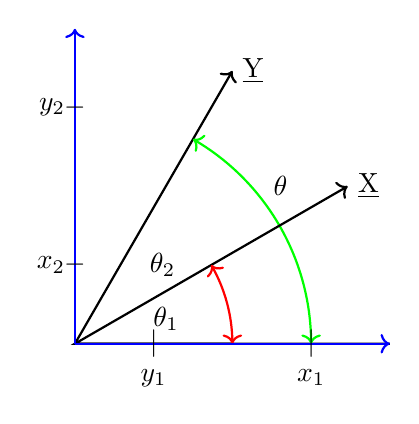
\begin{tikzpicture}[scale =4,=>stealth]
\coordinate (A) at (1,0);
\coordinate (B) at (0,0);
\coordinate (C) at (60:1cm);
\coordinate (D) at (0.5,0);
\coordinate (E) at (30:1cm);
%\coordinate (F) at (30:1cm);
%\coordinate (E) at (3,1);
\draw[->,thick] (A)--(B)--(C)
pic[thick,angle radius =3cm,draw = green,<->]{angle = A--B--C}node[right]{\underline{Y}};
\draw[->,thick] (D)--(B)--(E)
pic[thick,angle radius =2cm,draw=red,<->,"$\theta_1$"]{angle = D--B--E}node[right]{\underline{X}};
\draw(0.6,0.5)node[right]{$\theta$}
(0.35,0.25)node[left]{$\theta_2$};
\draw[thick,blue,->](0,0)--(0,1);
\draw[thick,blue,->](0,0)--(1,0);
\draw(0,0.25)node[]{$-$}
(0,0.75)node[]{$-$}
(0.25,0)node[]{$|$}
(0.75,0)node[]{$|$};
\draw(0,0.25)node[left]{$x_2$}
(0,0.75)node[left]{$y_2$}
(0.25,-0.05)node[below]{$y_1$}
(0.75,-0.05)node[below]{$x_1$};
\end{tikzpicture}
\end{figure}











In the figure:
\begin{enumerate}
\item $\theta = \theta_2 - \theta_1$

\item $\theta_2$ is associated with $\underline{Y}$

\item $\theta_1$ is associated with $\underline{X}$

\item $\frac{X_1}{L_x}= \cos \theta_1,  \frac{X_2}{L_x}= \sin \theta_1$

\item $\frac{Y_1}{L_y}= \cos \theta_2,  \frac{Y_2}{L_y}=\sin \theta_2$

\item Now
\begin{align*}
\cos 3\theta & = \cos ( \theta_2 - \theta_1)\\
& = \cos \theta_2\cos \theta_1 + \sin \theta_2\sin \theta_1\\\\
& = \frac{Y_1}{L_y}\cdot \frac{X_1}{L_x} + \frac{Y_2}{L_y}\cdot \frac{X_2}{L_x}\\
\end{align*}


\begin{align*}
\cos 3\theta & = \frac{X_1Y_1 + X_2Y_2}{L_XL_Y}=\frac{\underline{X}'\underline{Y}}{L_xL_y}\\\\
& = \frac{\underline{X}'\underline{Y}}{\sqrt{\underline{X}'\underline{X}}\sqrt{\underline{Y}'\underline{Y}}}\tag{4}\\
\end{align*}
\end{enumerate}


From relationship (4) we have the \,$\displaystyle{4.1\qquad  \theta = 0 \implies 1 = \frac{\underline{X}'\underline{Y}}{L_xL_y}\qquad\text{or}\quad  L_xL_y = \underline{X}'\underline{Y}}$\\\\

suggesting $\underline{Y} = t\underline{X}$ for some $t$ \,$\displaystyle{4.2\qquad  \theta = \frac{\pi}{2}\implies 0 = \frac{\underline{X}'\underline{Y}}{L_xL_y}\implies  \underline{X}'\underline{Y} = 0}$\\


suggesting $\underline{X}$ and $\underline{Y}$ are perpendicular.\\\\




\subsubsection{Projection}
If $\underline{X}$ and $\underline{Y}$ are two vectors the projection of $\underline{X}$ on $\underline{Y}$ is \,$\displaystyle{= \frac{\underline{X}'\underline{Y}}{\underline{Y}'\underline{Y}}\,\underline{Y}}$\\\\
( a vector on $\underline{Y}$) $\qquad (5)$\\

% DIAGRAM 3
\begin{figure}[H]
\centering
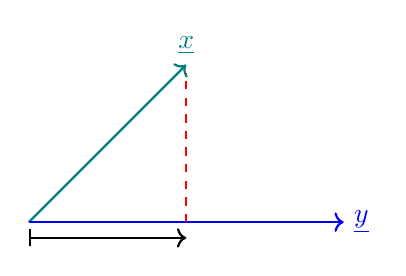
\begin{tikzpicture}[=>stealth]
\draw[thick,teal,->](0,0)--(2,2)node[above]{$\underline{x}$};
\draw[thick,blue,->](0,0)--(4,0)node[right]{$\underline{y}$};
\draw[thick,red,dashed](2,0)--(2,1.9);
\draw[|->,thick](0,-0.2)--(2,-0.2);
\end{tikzpicture}
\end{figure}


$$\frac{\underline{x}'\underline{y}}{L^2_Y}\,\underline{y}$$\\

















Note that\, $\displaystyle{\frac{\underline{X}'\underline{Y}}{L_yL_y}\, \underline{Y}= \frac{\underline{X}'\underline{Y}}{L_y}\cdot \frac{\underline{Y}}{L_y}=\frac{\underline{X}'\underline{Y}}{L_y}\cdot \mu_y}$\\\\

$\mu_y = \frac{\underline{Y}}{L_y}$ ( a unit vector in the direction of $\underline{Y}$). So $\frac{\underline{X}'\underline{Y}}{L_yL_y}\, \underline{Y} = L_x\cos \theta \frac{\underline{Y}}{L_y}$.\\

The length of the projection is 


\begin{align*}
\Bigg[\Bigg(\frac{\underline{X}'\underline{Y}}{L_y^2}\,\underline{Y}\Bigg)'\Bigg(\frac{\underline{X}'\underline{Y}}{L_y^2}\,\underline{Y}\Bigg)\Bigg]^{\frac{1}{2}}
 & = \frac{L_x L_y 
\begin{vmatrix}
\cos \theta\\
\end{vmatrix}  
 }{L_y}
  = L_x \begin{vmatrix}
 \cos \theta\\
 \end{vmatrix}\tag{6}\\
\end{align*}




\begin{table}[H]
\centering
\begin{tabular}{|c|cccc|}
\hline
Province & $1991_X$ & $1993_Y$ & $X\cdot Y$ & Pro $X$ on $Y$\\
\hline
&&&&\\
Central & 55.7 & 70.7 & 3938.0 & $+65.3$\\
&&&&\\
Copperbelt & 43.8 & 28.1 & 1230.8 & $-26.0$\\
&&&&\\
Eastern & 76.1 & 81.2 & 6179.3 & $-75.0$\\
&&&&\\
Luapula & 72.5 & 77.8 & 5640.5 & $-71.9$\\
&&&&\\
Lusaka & 18.7 & 24.3 & 454.4 & $+22.4$\\
&&&&\\
Northern & 75.9 & 71.5 & 5426.9 & $-66.0$\\
&&&&\\
N.Western & 64.5 & 75.5 & 4869.8 & $+69.7$\\
&&&&\\
Southern & 69.4 & 76.1 & 5281.3 & $+70.3$\\
&&&&\\
Western & 75.8 & 83.5 & 6329.3 & $+77.1$\\
\hline
\end{tabular}
\caption{}
\end{table}















$$\underline{X}'\underline{Y} = 39350.24$$

$$L^2_y = 42600.83$$

$$\frac{\underline{X}'\underline{Y}}{L^2_y}\,\underline{Y}$$\\\\\\








\subsubsection{Eigen Values and Eigen Vectors}
\begin{enumerate}
\item General result\\
If $A_{p\times p}$ is any square matrix then $$q(\lambda) = 
\begin{vmatrix}
A - \lambda I\\
\end{vmatrix}$$ is the $p^{\text{th}}$ order polynomial in $\lambda$. The $P$ roots of $q(\lambda)$, $\quad  \lambda_1,\ldots, \lambda_p$ possibly complex numbers, are called eigenvalues of matrix $A$.\\
Some of the $\lambda_i$ will be equal if $q(\lambda)$ has multiple roots. For each $i=1,2,\ldots, p$,\\
$\begin{vmatrix}
A - \lambda I\\
\end{vmatrix} = 0$, so $A - \lambda_i I$ is singular. Hence there exists a non-zero vector $\underline{e}$ satisfying \begin{equation}\tag{2}
A\underline{e} = \lambda \underline{e}
\end{equation} Any vector satisfying (2) is called an eigenvector of $A$ and $\begin{vmatrix}
A - \lambda I\\
\end{vmatrix} =  0$ is called the characteristic equation.

\item An eigenvector $\underline{e}$ with real entries is called standardized if $\underline{e}'\underline{e} = 1\qquad (3)$

\item Since the coefficients of $\lambda^p$ in $q(\lambda)$ is $(-1)^p$ we can write $q(\lambda)$ in terms of its roots as follows \begin{equation}\tag{4}
q(\lambda) = \prod^p_{i=1} (\lambda_i - \lambda)
\end{equation} and setting $\lambda = 0$ in (1) and (4) gives \begin{equation}\tag{5}
\begin{vmatrix}
A\\
\end{vmatrix}= \prod^p_{i=1} \lambda_i
\end{equation} i.e $\begin{vmatrix}
A\\
\end{vmatrix}$ is the product of the eigenvalues of A.

\item Matching the coefficients of $\lambda^{p-1}$ in equation (1) and (4) gives \begin{equation}\tag{6}
\sum^p_{i=1} a_{ij} = \sum^p_{i=1} \lambda_i = Tr(A)
\end{equation} $Tr(A)$ is the sum of eigenvalues of $A$.\\\\
\end{enumerate}



\begin{exa}
Consider the matrix $A = \begin{pmatrix}
1 & 3 & 0 \\
3 & 1 & 0\\
0 & 0 & 2\\
\end{pmatrix}$
\end{exa}


\begin{enumerate}
\item Determine
\begin{enumerate}
        \item eigenvalues $\lambda_1, \lambda_2, \lambda_3$
        
        \item eigenvectors
\end{enumerate}

\item Verify
\begin{enumerate}
     \item $\begin{vmatrix}
     A\\
     \end{vmatrix} = \prod \lambda_i$
     
     \item $Tr(A) = \sum \lambda_i$\\\\
\end{enumerate}
\end{enumerate}



\begin{solution}
Characteristic equation $\begin{vmatrix}
1-\lambda & 3 & 0 \\
3 & 1 -\lambda & 0\\
0 & 0 & 2-\lambda\\
\end{vmatrix}=0$
\end{solution}



\begin{align*}
(1-\lambda)(1-\lambda)(2-\lambda)-9(2-\lambda) & = 0\\
(2-\lambda)\big[(1-\lambda)^2-9\big] & = 0\\
(2-\lambda)(1-\lambda - 3) (1-\lambda + 3) & = 0\\
(2-\lambda)(-2-\lambda)(4-\lambda) & = 0\\
\end{align*}


$$\lambda = 2,  \lambda = 4,  \lambda = -2$$


\begin{enumerate}
\item
\begin{enumerate}
     \item $\lambda_1 = 2,  \lambda_2 = 4,  \lambda_3 = -2$
     
     \item $\lambda_1 = 2$
     \begin{align*}
     A\underline{e} & = 2 \underline{e}\qquad  (A\underline{e}  = \lambda \underline{e})\\\\
     \begin{pmatrix}
     1 & 3 & 0\\
     3 & 1 & 0\\
     0 & 0 & 2\\
     \end{pmatrix}\begin{pmatrix}
     e_1\\
     e_2\\
     e_3\\
     \end{pmatrix} & = 2\begin{pmatrix}
     e_1\\
     e_2\\
     e_3\\
     \end{pmatrix}\\
     \end{align*}
     

\begin{align*}
e_1 + 3e_2 & = 3e_1 \quad \cdots\quad  (i)\\
3e_1 + e_2 & = 2e_2\quad \cdots\quad  (ii)\\
     2e_3 & = 2e_3\quad  \cdots\quad  (iii)\\
\end{align*}

From $(ii)$ , $e_2=3e_1$ and using $(i)$ we obtain $$e_1 =0 \implies e_2 = 0$$
Choose $e_3 = 1$ so $\underline{e}_1 = \begin{pmatrix}
0, & 0, & 1\\
\end{pmatrix}'$\\\\



Alternatively: $\begin{pmatrix}
1 & 3 & 0\\
3 & 1 & 0\\
0 & 0 & 2\\
\end{pmatrix}\underline{e} = 2\underline{e}$

\begin{align*}
\implies \qquad  \Bigg[\begin{pmatrix}
1 & 3 & 0\\
3 & 1 & 0\\
0 & 0 & 2\\
\end{pmatrix} -2 I_3\Bigg] \underline{e} & = 0\\\\
\begin{pmatrix}
-1 & 3 & 0\\
3 & -1 & 0\\
0 & 0 & 0\\
\end{pmatrix}\underline{e} & = 0\\\\
\begin{pmatrix}
A^* & \underline{0}\\
\underline{0} & 0\\
\end{pmatrix}\begin{pmatrix}
\underline{e}_1\\
\underline{e}_2\\
\end{pmatrix} & = \begin{pmatrix}
\underline{0}\\
\underline{0}\\
\end{pmatrix}\quad  \cdots\quad  *\\
\end{align*}

From $*$ we obtain $e_1 = e_2 =0$ since a $
\begin{vmatrix}
A^*\\
\end{vmatrix}= \begin{vmatrix}
-1 & 3\\
-3 & -1\\
\end{vmatrix}\neq 0$ and $e_3$ can be chosen to be any value.\\\\




For $\lambda = 4$ $\qquad  \begin{pmatrix}
1 & 3 & 0\\
3 & 1 & 0\\
0 & 0 & 2\\
\end{pmatrix}\underline{e} =4\underline{e}$

\begin{align*}
e_1 + 3e_2 & = 4e_1 \quad \cdots\quad  (i)\\
3e_1 + e_2 & = 4e_2 \quad \cdots\quad  (ii)\\
2e_3 & = 4e_3       \quad  \cdots\quad  (iii)\\
\end{align*}

From $(iii)$, $2e_3 = 0 \implies e_3 = 0$ in $(i)$ $$3e_2 = 3e_1 \implies e_2 = e_1$$ the same as in $(ii)$. Choose $e_1 = e_2 = 1$ $$\underline{e}^*_2 = \begin{pmatrix}
1, & 1, & 0\\
\end{pmatrix}'$$
\begin{note}
$\begin{vmatrix}
\begin{vmatrix}
\underline{e}_2^*\\
\end{vmatrix}
\end{vmatrix} = \sqrt{2}$, but we require $e^*_2$ to be a unit vector, hence we normalize $\underline{e}^*_2$ to obtain
\end{note}
\begin{align*}
\underline{e}_2 & = \begin{pmatrix}
\frac{1}{\sqrt{2}}, & \frac{1}{\sqrt{2}}, & 0\\
\end{pmatrix}'\\\\
& = \begin{pmatrix}
\frac{\sqrt{2}}{2}, & \frac{\sqrt{2}}{2}, & 0 \\
\end{pmatrix}'\\
\end{align*}


For $\lambda = -2\qquad $ $\begin{pmatrix}
1 & 3 & 0\\
3 & 1 & 0\\
0 & 0 & 2\\
\end{pmatrix}\underline{e} = -2\underline{e}$


\begin{align*}
e_1 + 3e_2 & = -2e_1 \quad  \cdots\quad  (i)\\
3e_1 + e_2 & = -2e_2 \quad   \cdots\quad  (ii)\\
      2e_3 & = -2e_e \quad  \cdots\quad  (iii)\\
\end{align*}

From $(iii)$ we get $4e_3 = 0 \implies e_3 =0$\\

$(i)$ and $(ii)$ $\implies\quad 
\left.\begin{aligned}
3e_1 + 3e_2 & = 0\\
3e_1 + 3e_2 & = 0\\
\end{aligned}
\right\}\quad  \cdots\quad  *
$\\

from $*$ we get $e_1 = -e_2$. Choose $e_1 = 1 \implies e_2 = -1$ . Hence $\underline{e}^*_3 = \begin{pmatrix}
1, & -1, & 0\\
\end{pmatrix}'$

$$\text{Thus}\qquad  \underline{e}_3 = \begin{pmatrix}
\frac{1}{\sqrt{2}}, & -\frac{1}{\sqrt{2}}, & 0\\
\end{pmatrix}'$$\\




\begin{table}[H]
\centering
\begin{tabular}{ccccc}
$\lambda_1 = 2$ && $\lambda_2 = 4$ && $\lambda_3 = -2$\\
&&&&\\
$\displaystyle{
\underline{e}_1 = 
\begin{pmatrix}
0\\
0\\
1\\
\end{pmatrix}
}$ && $\displaystyle{\underline{e}_2 = 
\begin{pmatrix}
1/\sqrt{2}\\
1/\sqrt{2}\\
0\\
\end{pmatrix}
}$  && $\displaystyle{\underline{e}_3=
\begin{pmatrix}
1/\sqrt{2}\\
-1/\sqrt{2}\\
0\\
\end{pmatrix}
}$
\end{tabular}
\end{table}



\begin{note}
\begin{align*}
\underline{e}_1 \cdot \underline{e}_2 & = 0 (1/\sqrt{2}) + 0(1/\sqrt{2}) + 1 (0) = 0\\
\underline{e}_1 \cdot \underline{e}_3 & = 0(1\sqrt{2})   + 0(-1/\sqrt{2}) + 1 (0) = 0\\
\underline{e}_2 \cdot \underline{e}_3 & = \frac{1}{\sqrt{2}}(1/\sqrt{2}) + \frac{1}{\sqrt{2}}(-1\sqrt{2}) + 0(0) = 0\\
\end{align*}
\end{note}



$$\implies \qquad  \underline{e}_1 \perp \underline{e}_2,  \underline{e}_1 \perp \underline{e}_3,  \underline{e}_2 \perp \underline{e}_3$$\\
\end{enumerate}



\item
\begin{enumerate}
      \item \begin{align*}
      \begin{vmatrix}
      A\\
      \end{vmatrix} & = \begin{vmatrix}
      1 & 3\\
      3 & 1\\
      \end{vmatrix}(2) = (1-9)(2)\\\\
      & = (-8)(2)\\\\
      & = \prod^3_{i=1}\lambda_i = \lambda_1 \cdot \lambda_2 \cdot \lambda_3\\
      & = 2(4)(-2)\\
      & = -16\\
      \end{align*}
      
      
      
      
\item \begin{align*}
Tr(A) & = Tr
\begin{pmatrix}
1 & 3 & 0\\
3 & 1 & 0\\
0 & 0 & 2\\
\end{pmatrix}\\\\
& = 1 + 1 + 2 = \sum^3_{i=1} \lambda_i = \\\\
& = 4 = 2 + 4 + (-2)\\
\implies \qquad  & 4  = 4\\\\
\end{align*}
\end{enumerate}
\end{enumerate}











\subsection{Spectral Decomposition}
The study of the variation and interrelationships in multivariate data is often based on distances and the assumption of multivariate normally data squared distances and multivariate normal density can be expressed in terms of matrix products called quadratic forms. \\
Consequently, quadratic forms play a central role in multivariate analysis. One important result involves the expansion of the symmetric matrix into what is known as spectral decomposition.\\\\



\begin{thm}[Spectral Decomposition theorem of Jordan Decomposition theorem]
Any symmetric matrix $A_{p\times p}$ can be written as $$A = E\Delta E' = \sum \lambda_i\underline{e}_i\underline{e}_j'$$ where $\Delta$ is a diagonal matrix of eigenvalues of $A$ and $E$ is an orthogonal matrix whose columns are standardized eigenvectors.\\\\
\end{thm}


\begin{proof}
Suppose that we can find orthognormal vectors $\underline{e}_1,\underline{e}_2,\ldots,\underline{e}_p$ such that $$A \underline{e}_i = \lambda_i \underline{e}_i\qquad i = 1,2,\ldots, p$$
for some numbers $\lambda_i$. Then $$\underline{e}'_jA\underline{e}_i = \lambda_i \underline{e}'_j \underline{e}_i = \begin{cases}
\lambda_i & i = j\\\\
0 & i\neq j\\
\end{cases}$$ or in matrix form we have $$E'AE = \Delta\quad \cdots\quad  *$$ and pre and post multiply $*$ by $E$ and $E'$ gives the result $$A = E\Delta E'$$ where $EE' =  E'E = I_p$.\\
It is clear that $\Delta$ has the same eigenvalues as $A$.\\\\
\end{proof}



\begin{exa}
Recall that in the previous example we had $\lambda_1 = 2,  \lambda_2 = 4,  \lambda_3 = -2$
$$\underline{e}_1 = \begin{pmatrix}
0, & 0, & 1\\
\end{pmatrix}',  \underline{e}_2 = \begin{pmatrix}
\frac{1}{\sqrt{2}}, & \frac{1}{\sqrt{2}}, & 0\\
\end{pmatrix}',  \underline{e}_3 = \begin{pmatrix}
\frac{1}{\sqrt{2}}, & -\frac{1}{\sqrt{2}}, & 0\\
\end{pmatrix}'$$\\
\end{exa}


$A = \begin{pmatrix}
1 & 3 & 0\\
3 & 1 & 0\\
0 & 0 & 2\\
\end{pmatrix}$ , a symmetric matrix\\

\begin{align*}
& = 2 \begin{pmatrix}
0\\
0\\
1\\
\end{pmatrix}\begin{pmatrix}
0, & 0, & 1\\
\end{pmatrix}
+ 4 \begin{pmatrix}
1/\sqrt{2}\\
1/\sqrt{2}\\
0\\
\end{pmatrix}\begin{pmatrix}
1/\sqrt{2}, & 1/\sqrt{2}, & 0\\
\end{pmatrix} -2 \begin{pmatrix}
1/\sqrt{2}\\
-1/\sqrt{2}\\
0\\
\end{pmatrix}\begin{pmatrix}
1/\sqrt{2}, & -1/\sqrt{2}, & 0\\
\end{pmatrix}\\\\
& = 2\begin{pmatrix}
0 & 0 & 0\\
0 & 0 & 0\\
0 & 0 & 1\\
\end{pmatrix} +4\begin{pmatrix}
\frac{1}{2} & \frac{1}{2} & 0\\\\
\frac{1}{2} & \frac{1}{2} & 0\\\\
  0          &     0        & 0\\
\end{pmatrix}-2\begin{pmatrix}
\frac{1}{2} & -\frac{1}{2} & 0\\\\
-\frac{1}{2} & \frac{1}{2} & 0\\\\
    0        &     0         & 0\\
\end{pmatrix}\\\\
& = \begin{pmatrix}
1 & 3 & 0\\
3 & 1 & 0\\
0 & 0 & 2\\
\end{pmatrix}\\\\
\end{align*}




\textbf{1.9.2}\\
Using the spectral decomposition it is rather easy to show that a $p \times p$ symmetric matrix. $A$ is a $+ve$ definite matrix if and only if every eigenvalue of $A$ is $+ve$. It is non-negative definite matrix if and only if all of its eigenvalues are greater than or equal to zero.\\\\

\subsubsection{Distance}
We can think of $A$ as a matrix of transformation and the square distance from a vector $\underline{X}$ to an arbitrary fixed $\underline{\mu}' = \begin{pmatrix}
\mu_1, & \cdots, & \mu_p\\
\end{pmatrix}$ is given by $$d\big(\underline{X},\underline{\mu}\big) = \big(\underline{X}-\underline{\mu}\big)' A\big(\underline{X}-\underline{\mu}\big)$$ Using spectral decomposition we express the distance as $$d\big(\underline{X},\underline{\mu}\big) =\big(\underline{X}-\underline{\mu}\big)'E\Delta E'\big(\underline{X}-\underline{\mu}\big)=\big[E'\big(\underline{X}-\underline{\mu}\big)\big]'\Delta E'\big(\underline{X}-\underline{\mu}\big)$$

Let $\underline{Y} = E'\big(\underline{X}-\underline{\mu}\big)$ $$d\big(\underline{X},\underline{\mu}\big) = \underline{Y}\Delta \underline{Y}= \sum^p_{i=1}\lambda_iY_i^2$$

For points at the distance of $C$ units, we have the following $$\sum^p_{i=1}\lambda_iY^2_i = C^2$$
which form an equation of an ellipsoid centered at $\underline{\mu} = \begin{pmatrix}
\mu_1, & \cdots, & \mu_p\\
\end{pmatrix}'$ and have axes $\pm C\sqrt{\lambda_i}\underline{e}_i$, where $A\underline{e}_i = \lambda_i \underline{e}_i$.



% DIAGRAM 4
\begin{figure}[H]
\centering
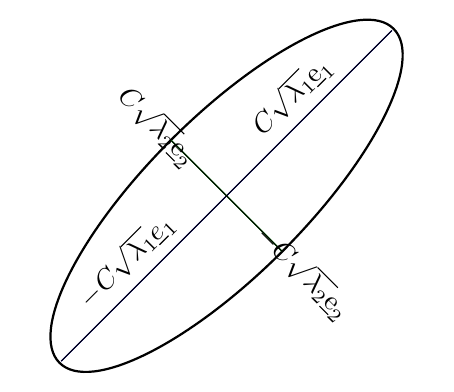
\begin{tikzpicture}[=>stealth]
\draw[thick,rotate=45](0,0)ellipse[x radius =3,y radius = 1];
\draw[domain =-2.1:2.1,smooth,variable=\x,blue]plot({\x},{\x});
\draw[domain=-0.7:0.7,smooth,variable=\x,green]plot({\x},-{\x});
\draw(-2.1,-2.1)--node[above,sloped]{$-C\sqrt{\lambda_1}\underline{e}_1$}(0,0);
\draw(0,0)--node[above,sloped]{$C\sqrt{\lambda_1}\mathrm{\underline{e}}_1$}(2.1,2.1);
\draw(-0.7,0.7)--node[left,sloped]{$C\sqrt{\lambda_2}\mathrm{\underline{e}}_2$}(0,0);
\draw(0,0)--node[right,sloped]{$-C\sqrt{\lambda_2}\mathrm{\underline{e}}_2$}(0.7,-0.7);
\end{tikzpicture}
\end{figure}












\subsubsection{Square Root Matrix}
The spectral decomposition allows us to express the inverse of the square matrix in terms of its eigenvalues , vectors and thus leads to a useful square matrix.\\\\



\begin{result}
Recall that under the spectral decomposition a square matrix $A_{p\times p}$ can be expressed as\\ $A = E\Delta E'$ where $EE' = E'E = I$ so that $E^{-1} = E'$\\\\
\end{result}
 
 
Now
\begin{align*}
A^{-1} & = \big(E\Delta E'\big)^{-1}\qquad   \big(ABC\big)^{-1} = C^{-1}B^{-1}A^{-1}\\
       & = \big(E'\big)^{-1}\Delta^{-1} E^{-1}\\
       & = \big(E^{-1}\big)^{-1}\Delta^{-1}E'\\
       & = E\Delta^{-1}E'\\
\end{align*} 


\begin{equation}\tag{1}
\text{So}\quad  A^{-1} = E\Delta^{-1} E' = \sum^p_{i=1} \frac{1}{\lambda_i}\underline{e}_i\underline{e}'_i
\end{equation}


Let $\Delta^{1/2}$ denote the diagonal matrix with $\sqrt{\lambda_i}$ as the $i^{\text{th}}$ diagonal element

$$\text{e.g}\quad  p=2\qquad  \Delta = \begin{pmatrix}
\lambda_1 & 0 \\
0 & \lambda_2\\
\end{pmatrix}$$

$$\Delta^{1/2} = \begin{pmatrix}
\sqrt{\lambda_1} & 0\\
0 & \sqrt{\lambda_2}\\
\end{pmatrix}$$
Then the matrix
\,$\displaystyle{\sum^p_{i=1}\sqrt{\lambda_i}\underline{e}_i\underline{e}'_j = E \Delta^{1/2}E'}\,$ is called the square root of $A$ is denoted by $A^{1/2}$.\\\\







The square - root matrix \begin{equation}\tag{2}
A^{1/2} = \sum^p_{i=1}\lambda^{1/2}_i\underline{e}_i\underline{e}'_j = E\Delta^{1/2} E'
\end{equation} has the following properties
\begin{enumerate}
\item $\big(A^{1/2}\big)' = A^{1/2}$ 
$$\text{Since}\quad \big(A^{1/2}\big)' = \big(E\Delta^{1/2}E'\big)' = \big(E'\big)'\big(\Delta^{1/2}\big)'E' = E\Delta^{1/2}E'$$\\

\item $A^{1/2}\cdot A^{1/2} = A$
\begin{align*}
\text{Since}\qquad   A^{1/2}\cdot A^{1/2} & = \big(E\Delta^{1/2}E'\big)\big(E\Delta^{1/2}E'\big) = E\Delta^{1/2}E'E\Delta^{1/2}E'\\
& = E\Delta^{1/2}I\Delta^{1/2}E'\\
& = E \Delta^{1/2}\Delta^{1/2}E'\\
& = E \Delta E'\\
& = A\\
\end{align*}

\item $\displaystyle{\big(A^{1/2}\big)^{-1} = \sum^p_{i=1}\frac{1}{\sqrt{\lambda_i}}\underline{e}_i\underline{e}_j' = E\Delta^{-1/2}E' = A^{-1/2}}$ where $\Delta^{-1/2}$ is a diagonal matrix with $\frac{1}{\sqrt{\lambda_i}}$ has the $i^{\text{th}}$ diagonal element.\\

\item $A^{1/2}\cdot A^{-1/2} = A^{-1/2}\cdot A^{1/2} = I$\\

\item $\displaystyle{A^{-1/2}\cdot A^{-1/2}= A^{-1}}$ where $\big(A^{1/2}\big)^{-1} = A^{-1/2}$\\\\
\end{enumerate}



\begin{exa}
Let $A = \begin{pmatrix}
4 & \sqrt{3}\\
\sqrt{3} & 2\\
\end{pmatrix}$. So $A' = A$\\\\
\end{exa}

Characteristic function $\begin{vmatrix}
4 - \lambda & \sqrt{3}\\
\sqrt{3} & 2-\lambda\\
\end{vmatrix} = 0$
\begin{align*}
\implies\qquad  (4 - \lambda) (2 - \lambda) - 3 & = 0\\
\lambda^2 - 6\lambda + 5 & =0\\
\implies\quad  (\lambda -5)(\lambda - 1) & =0\\
\end{align*}

$$\therefore\qquad  \lambda_1 =5,  \lambda_2 = 1$$











\pagebreak

\textbf{eigenvectors}\\

For $\lambda = 5$
\begin{align*}
A\underline{e}_i & = \lambda_i \underline{e}_i\\\\
\begin{pmatrix}
4 & \sqrt{3}\\
\sqrt{3} & 2\\
\end{pmatrix}\begin{pmatrix}
e_1\\
e_2\\
\end{pmatrix} & = 5\begin{pmatrix}
e_1\\
e_2\\
\end{pmatrix}
\end{align*}


\begin{align*}
4e_1 + \sqrt{3}e_2 & = 5e_1\\
\sqrt{3}e_1 + 2e_2 & = 5e_2\\
\end{align*}

$$\implies\qquad  e_1 = \sqrt{3}e_2$$


Choose $e_2 =1,$ $\quad  e_1 = \sqrt{3}\qquad \implies \underline{e}_1^* = 
\begin{pmatrix}
\sqrt{3}, & 1\\
\end{pmatrix}'$ 
$$\underline{e}_1 = \begin{pmatrix}
\frac{\sqrt{3}}{2}, & \frac{1}{2}\\
\end{pmatrix}'$$\\\\






For $\lambda = 1$
$$A\underline{e}_2 = \lambda_2 \underline{e}_2$$

\begin{align*}
4e_1 + \sqrt{3}e_2 & = e_1\\
\sqrt{3}e_1 + 2e_2 & = e_2\\
\end{align*}

$$\implies \qquad  \sqrt{3}e_1 = -e_2$$

Choose $e_1 =1,  e_2 = -\sqrt{3}\qquad  \implies \underline{e}^*_2 = \begin{pmatrix}
1, & -\sqrt{3}\\
\end{pmatrix}'$

$$\underline{e}_2 = \begin{pmatrix}
\frac{1}{2}, & -\frac{\sqrt{3}}{2}\\
\end{pmatrix}'$$\\


$$E = \begin{pmatrix}
\frac{\sqrt{3}}{2} & \frac{1}{2}\\\\
\frac{1}{2} & -\frac{\sqrt{3}}{2}\\
\end{pmatrix}\qquad 
\Delta = \begin{pmatrix}
5 & 0\\
0 & 1\\
\end{pmatrix}
$$\\



Square root of $A$
\begin{align*}
A^{1/2} & = E\Delta^{1/2}E'\\\\
A^{1/2} & = \begin{pmatrix}
\frac{\sqrt{3}}{2} & \frac{1}{2}\\\\
\frac{1}{2} & -\frac{\sqrt{3}}{2}\\
\end{pmatrix}\begin{pmatrix}
\sqrt{5} & 0\\
0 & 1\\
\end{pmatrix}\begin{pmatrix}
\frac{\sqrt{3}}{2} & \frac{1}{2}\\\\
\frac{1}{2} & -\frac{\sqrt{3}}{2}\\
\end{pmatrix}\\\\
& = \begin{pmatrix}
\frac{\sqrt{15}}{2} & \frac{1}{2}\\\\
\frac{\sqrt{5}}{2} & -\frac{\sqrt{3}}{2}\\
\end{pmatrix}\begin{pmatrix}
\frac{\sqrt{3}}{2} & \frac{1}{2}\\\\
\frac{1}{2} & -\frac{\sqrt{3}}{2}\\
\end{pmatrix}\\\\
& = \begin{pmatrix}
\frac{\sqrt{45} + 1}{4} & \frac{\sqrt{15}-\sqrt{3}}{4}\\\\
\frac{\sqrt{15}-\sqrt{3}}{4} & \frac{\sqrt{5}+3}{4}\\\\
\end{pmatrix}
\end{align*}




\textbf{Verifications}
\begin{enumerate}
\item $\big(A^{1/2}\big)' = A^{1/2}$\\


\item $$A^{1/2}\cdot A^{1/2} = 
\begin{pmatrix}
\frac{\sqrt{45} + 1}{4} & \frac{\sqrt{15}-\sqrt{3}}{4}\\\\
\frac{\sqrt{15}-\sqrt{3}}{4} & \frac{\sqrt{5}+3}{4}\\\\
\end{pmatrix}
\begin{pmatrix}
\frac{\sqrt{45} + 1}{4} & \frac{\sqrt{15}-\sqrt{3}}{4}\\\\
\frac{\sqrt{15}-\sqrt{3}}{4} & \frac{\sqrt{5}+3}{4}\\\\
\end{pmatrix}
$$\\
\end{enumerate}






\begin{align*}
a_{11} & = \Bigg(\frac{\sqrt{14}+1}{4}\Bigg)^2 + \Bigg(\frac{\sqrt{15}-\sqrt{3}}{4}\Bigg)^2\\\\
       & = \frac{45 + 1 + 2\sqrt{45}}{16} + \frac{15 + 3 - 2\sqrt{45}}{16}\\\\
       & = \frac{64}{16}\\\\
       & =4\\
\end{align*}






















\begin{align*}
a_{12} & = \frac{(\sqrt{45}+1)(\sqrt{15}-\sqrt{3})}{16}+\frac{(\sqrt{15}-\sqrt{3})(\sqrt{5}+3)}{3}=a_{21}\\
       & = \frac{3\sqrt{75}-3\sqrt{15}+\sqrt{15}-\sqrt{3}}{16}+ \frac{\sqrt{75}+3\sqrt{15}-\sqrt{15}-3\sqrt{3}}{16}\\
       & = \frac{4\sqrt{75}-4\sqrt{3}}{16}\\
       & = \frac{5\sqrt{3}-\sqrt{3}}{4}\\
       & = \sqrt{3}\\
\end{align*}




\begin{align*}
a_{22} & = \Bigg(\frac{\sqrt{15}-\sqrt{3}}{4}\Bigg)\Bigg(\frac{\sqrt{15}-\sqrt{3}}{4}\Bigg)+\Bigg(\frac{\sqrt{5}+3}{4}\Bigg)\Bigg(\frac{\sqrt{5}+3}{4}\Bigg)\\ & = \frac{15-\sqrt{15}\sqrt{3}-\sqrt{15}\sqrt{3}+3}{16}+\frac{5+3\sqrt{5}+3\sqrt{5}+9}{16}\\
         & = \frac{15-2\sqrt{45}+3+5+6\sqrt{5}+9}{16}\\
         & = \frac{32-6\sqrt{5}+6\sqrt{5}}{16}\\
         & = 2\\ 
\end{align*}


$$
\begin{pmatrix}
4 & \sqrt{3}\\
\sqrt{3} & 2\\
\end{pmatrix}
= A\qquad \text{Hence}\quad  A^{1/2}A^{1/2} = A
$$








\pagebreak
%\chapter{\textcolor{red}{RANDOM VECTORS}}

\subsection{Practice Problems}

\begin{problem}
Let $A$ be partitioned as
$A = \begin{pmatrix} A_{11} & A_{12}\\ A_{21} & A_{22}\end{pmatrix}$
with $A_{11}$ non-singular. Show that
$$\left|A\right| = \left|A_{11}\right|\,
\left|A_{22}-A_{21}A_{11}^{-1}A_{12}\right|.$$
\emph{Where to start: write $A = BD$ with $B$ block lower triangular and $D$
block upper triangular, and use $|BD| = |B||D|$. The second factor is the Schur
complement, which reappears as a conditional covariance in Section~5.1.}
\end{problem}

\begin{problem}
Prove that $\operatorname{tr}(AB) = \operatorname{tr}(BA)$ whenever both
products are defined, and deduce that
$\operatorname{tr}(P\Lambda P') = \operatorname{tr}(\Lambda)$ for orthogonal
$P$. This is the identity behind Theorem~4.6.
\end{problem}

\begin{problem}
The centring matrix is $H = I - \tfrac{1}{n}\underline{1}\,\underline{1}'$.
Show that $H$ is symmetric and idempotent, that $H\underline{1}=\underline{0}$,
and that $\operatorname{tr}(H) = n-1$. Explain what each of these three facts
says about what $H$ does to a data matrix.
\end{problem}

\begin{solution}
Symmetry is immediate since $\underline{1}\,\underline{1}'$ is symmetric. For
idempotency,
$$H^{2} = I - \tfrac{2}{n}\underline{1}\underline{1}'
+ \tfrac{1}{n^{2}}\underline{1}\left(\underline{1}'\underline{1}\right)\underline{1}'
= I - \tfrac{2}{n}\underline{1}\underline{1}' + \tfrac{1}{n}\underline{1}\underline{1}' = H,$$
using $\underline{1}'\underline{1}=n$. Then
$H\underline{1} = \underline{1}-\tfrac{1}{n}\underline{1}(n) = \underline{0}$,
and $\operatorname{tr}(H) = n - \tfrac{1}{n}\operatorname{tr}(\underline{1}\underline{1}')
= n-1$.

Reading them in order: $H$ subtracts the column means; applying it twice does
nothing more, because once centred a column is already centred; a constant
column is annihilated entirely; and one degree of freedom is spent on the mean,
which is the $n-1$ that appears in the divisor of $S$.
\end{solution}

\begin{problem}
Show that a symmetric matrix $A$ is positive definite if and only if every
eigenvalue is strictly positive, and that $\left|A\right| = \prod\lambda_i$.
\end{problem}

\begin{problem}
Obtain the spectral decomposition of
$S = \begin{pmatrix} 4 & 1\\ 1 & 4\end{pmatrix}$, and verify both
$\left|S\right| = \lambda_1\lambda_2$ and
$\operatorname{tr}(S) = \lambda_1+\lambda_2$.
\end{problem}

\begin{solution}
$\left|S-\lambda I\right| = (4-\lambda)^{2}-1 = 0$ gives $\lambda_1=5$ and
$\lambda_2=3$, with normalised eigenvectors $(1,1)'/\sqrt2$ and
$(1,-1)'/\sqrt2$. Hence
$$S = 5\,\tfrac12\begin{pmatrix}1&1\\1&1\end{pmatrix}
+ 3\,\tfrac12\begin{pmatrix}1&-1\\-1&1\end{pmatrix}.$$
Then $\lambda_1\lambda_2 = 15 = 16-1 = \left|S\right|$ and
$\lambda_1+\lambda_2 = 8 = 4+4 = \operatorname{tr}(S)$.
\end{solution}

\begin{problem}
For $\Sigma$ positive definite, define the symmetric square root
$\Sigma^{1/2} = P\Lambda^{1/2}P'$ and verify that
$\Sigma^{1/2}\Sigma^{1/2}=\Sigma$ and that $\Sigma^{1/2}$ is symmetric. Where is
this matrix used later in the course?
\end{problem}

\begin{problem}
Show that if $A$ is $n\times p$ with $n<p$ then $A'A$ is singular. Relate this
to the statement in Section~5.3 that a multivariate analysis requires more
observations than variables.
\end{problem}

\section{Basic Properties of Random Vectors}
Let $\underline{X}'=\begin{pmatrix}
x_1, & x_2, & \cdots, & x_p\\
\end{pmatrix}
$ be a random vector. Then
\begin{enumerate}
\item The cumulative distribution function (CDF) is the function $F$ defined by $F(\underline{X}')$
\begin{equation}\tag{1}
F(\underline{X}^0)=Pr\big(\underline{X}'\leq \underline{X}^0\big) = Pr\big(x_1\leq x_1^0, x_2\leq x_2^0, \ldots, x_p\leq x_p^0\big)
\end{equation} 


%DIAGRAM 5
\begin{figure}[H]
\centering
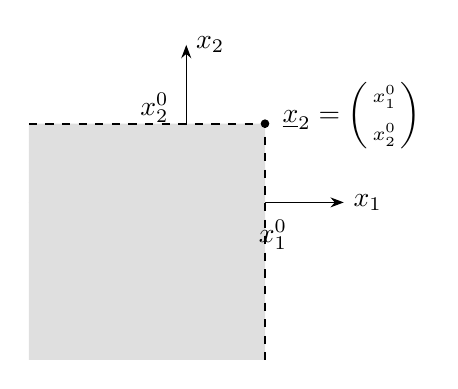
\begin{tikzpicture}[=>stealth]
\draw[-Stealth](-2,0)--(2,0)node[right]{$x_1$};
\draw[-Stealth](0,-2)--(0,2)node[right]{$x_2$};
\path[fill=gray!25](-2,1)--(1,1)--(1,-2)|-(-2,-2);
\draw[dashed,thick](-2,1)--(1,1)--(1,-2);
\draw(1,1)node[shape = circle,draw,scale=0.01cm,fill=black!]{};
\draw(1.1,1.1)node[right]{$\underline{x}_2 = \left(\begin{smallmatrix}
x_1^0\\\\
x_2^0\\
\end{smallmatrix}\right)$};
\draw(1.1,-0.1)node[below]{$x_1^0$}
(-0.1,1.2)node[left]{$x^0_2$};
\end{tikzpicture}
\end{figure}




$$Pr(\underline{X}\leq x_2^0) = Pr(x_1\leq x_1^0, x_2\leq x^0_2)$$














There are two cases continuous and discrete distributions.
\begin{enumerate}
\item $\displaystyle{F(\underline{X} = \int^{\infty}_{-\infty}f(\underline{U})d\underline{U}}\qquad (2)$ where $d\underline{U}=du_1\cdot du_2\cdot\cdots du_p$
$$\int^{\underline{X}}_{-\infty} = \int^{x_1}_{-\infty}\int^{x_2}_{-\infty}\cdots\int^{x_p}_{-\infty}$$

\item $\displaystyle{\int^{\infty}_{-\infty}f\big(\underline{U}\big)d\underline{U}=1}$\\\\
\end{enumerate}





A random vector $\underline{X}$ is discrete if there exists a probability mass function (Pmf) $f\big(\underline{U}\big)$ such that 
\[f\big(\underline{X}_j\big) =
\begin{cases}
Pr\big(\underline{X}=\underline{X}_j & j=1,2,\ldots\\\\
0, & \text{otherwise}\\
\end{cases}
\]\\
\end{enumerate}






\subsection{Marginal and Conditional Distribution Functions}
Consider the partitioned vector $\underline{X}'=\begin{pmatrix}
\underline{X}_1, & \underline{X}_2\\
\end{pmatrix}$
where $\underline{X}_1$ and $\underline{X}_2$ have $k$ and $p-k$ elements, respectively $(k<p)$ . Let $\underline{X}$ have a joint pdf $f\big(\underline{X}\big)$. Then marginal pdf of $\underline{X}_1$ is given by 
\begin{equation}\tag{4}
f_1\big(\underline{X}_1\big) = \int^{\infty}_{-\infty} f\big(\underline{X}_1,\underline{X}_2\big)d\underline{X}_2
\end{equation}
the marginal pdf of $\underline{X}_2$ is defined similarly as 


$$f_2\big(\underline{X}_2\big) = \int^{\infty}_{-\infty} f\big(\underline{X}_1,\underline{X}_2\big)d\underline{X}_1$$\\




$\bullet$ For the given value of $\underline{X}_1$ , say $\underline{X}_1 = \underline{X}^0_1$. The conditional pdf of $\underline{X}_2$  given $\underline{X}_1 = \underline{X}_1^0$ is \begin{equation}\tag{5}
f\big(\underline{X}_2/\underline{X}_1=\underline{X}_1^0\big) = \frac{f\big(\underline{X}_1^0,\underline{X}_2\big)}{f_1\big(\underline{X}_1^0\big)}
\end{equation}
where $f_1\big(\underline{X}_1^0\big) \neq 0$ .\\

The conditional pdf of $\underline{X}_1$ given $\underline{X}_2 = \underline{X}_2^0$ is defined similarly.\\\\

\begin{exa}
Let $X_1$ and $X_2$ be random variables with a joint pdf  
\[f\big(X_1,X_2\big) =
\begin{cases}
1 + \alpha (2x_1-1)(2x_2-1), & 0<x_1,x_2<1\quad  -1\leq \alpha \leq 1\\\\
0, & \text{otherwise}\\
\end{cases}
\]
\end{exa}


\begin{enumerate}
\item Is $f\big(X_1,X_2\big)$ a density function?
\item If yes, what is
\begin{enumerate}
       \item $f_1\big(X_1\big)$?
       \item $f_2\big(X_2\big)$?\\
\end{enumerate}
\end{enumerate}



\begin{solution}
\begin{enumerate}
\item 
\begin{align*}
\int^1_0\int^1_0f\big(X_1,X_2\big) dX_1dX_2 & = \int^1_0\int^1_0 \big(1+\alpha(2x_1-1)(2x_2-1)\big)dx_1dx_2\\
                                            & = \int^{1,1}_{0,0} dx_1dx_2 + \alpha \int^{1,1}_{0,0}(2x_1-1)(2x_2-1)dx_1dx_2\\
                                            & = 1 + \alpha \int^1_0 (2x_2-1)(x^2_1-x_1)\big|^1_0dx_2\\
                                            & = 1 + \alpha \int^1_0(2x_2-1)(0)dx_2\\
                                            & = 1\\
\end{align*}


\item
\begin{enumerate}
      \item $\displaystyle{f_1\big(X_1\big) = \int_{x_2}f(x_1,x_2)dx_2}= 1\quad  0<x_1<1$\\
      \item $\displaystyle{f_2\big(X_2\big) = \int_{x_1} f\big(x_1,x_2\big)dx_1=
\begin{cases}      
      1, & 0<x_2 < 1\\\\
      0, & \text{Otherwise}\\
\end{cases}      
      }$\\\\
\end{enumerate}
\end{enumerate}
\end{solution}






\subsection{Independence}
\begin{thm}
If $\underline{X}_1$  and $\underline{X}_2$ are statistically independent then 
\begin{enumerate}
\item $f\big(\underline{X}\big) = f_1\big(\underline{X}_1\big)\cdot f_2\big(\underbrace{X}_2\big)$, where $\underline{X} =\begin{pmatrix}
\underline{X}'_1, & \underline{X}'_2\\
\end{pmatrix}$

\item $f\Big(\underline{X}_2/\underline{X}_1\Big) = f_2\big(\underline{X}_2\big)$ or $f\Big(\underline{X}_1/\underline{X}_2\Big) =f_1\big(\underline{X}_1\big)$\\\\
\end{enumerate}
\end{thm}


\begin{exa}
$X_1$ and $X_2$ in the previous example are dependent since $$f_1\big(X_1\big)f_2\big(X_2\big) = 1 \neq 1 + (2x_1-1)(2x_2-1)\quad  0<x_1,x_2<1\quad  -1\leq \alpha < 1$$\\\\
\end{exa}




\subsection{Population Moments}
\begin{enumerate}
\item[(A).] \textbf{EXPECTATION:} If $\underline{X}$ is a random variable with pdf $f\big(\underline{X}\big)$ then the expectation or mean of a scalar-valued function $g(\underline{X})$ is defined as \begin{equation}\tag{1}
E\Big(g(\underline{X})\Big) = \int^{\infty}_{-\infty} g(\underline{X})f\big(\underline{X}\big) d\underline{X}
\end{equation}
\item[(B).] Properties of the expectation 
\begin{enumerate}
          \item Linearity \begin{equation}\tag{2}
E[ag_1(\underline{X}) + b g_2(\underline{X})]= aE\Big(g_1(\underline{X})\Big) + bE\Big(g_2(\underline{X})\Big)
\end{equation}
          \item Partition $\underline{X}' = \begin{pmatrix}
          \underline{X}_1', & \underline{X}_2'\\
          \end{pmatrix}$ . The expectation of a function of $\underline{X}_1$ may be written in terms of marginal distributions $\underline{X}_1$ as follows 
\begin{align*}
E\big\{g(\underline{X}_1)\big\} & = \int^{\infty}_{-\infty} g(\underline{X}_1)\cdot f(\underline{X}) d\underline{X}\\
                                & = \int^{\infty}_{-\infty} g(\underline{X}_1)\cdot f_1(x_1)dx_1
\end{align*}
where $f_1(x_1)$ is known, the second expression is useful for computation.\\

        \item If $\underline{X}_1$ and $\underline{X}_2$ are independent and $g_i(\underline{X}_i)$ is a function of $\underline{x}_i$ alone $i=1(1,2)$ then $$E\big[g_1(\underline{x}_1)g_2(\underline{x}_2)\big] = E\big[g_1(\underline{x}_1)\big]E\big[g_2(\underline{x}_2)\big]$$ more generally the expectation of the matrix valued (or vector valued) functions of $X$.\\
        $G(\underline{X}) = \Big(g_{ij}(\underline{X})\Big)$ is defined to be the matrix
\begin{align*}
E\big[G(\underline{X})\big] & = \Bigg(E\big[g_{ij}(\underline{X})\big]\Bigg)\\\\
G(\underline{X}) & = \begin{pmatrix}
g_{11}(\underline{X}) & g_{12}(\underline{X})\\\\
g_{21}(\underline{X}) & g_{22}(\underline{X})\\
\end{pmatrix}\\\\
E\big[G(\underline{X})\big] &  = \begin{pmatrix}
E\, g_{11}(\underline{X}) & E\, g_{12}(\underline{X})\\
                                      & \\
E\, g_{21}(\underline{X}) & E\, g_{22} (\underline{X})\\
\end{pmatrix}\\
\end{align*}

             \item The vector $E(\underline{X}) = \underline{\mu}$ is called the population mean vector of $\underline{X}$. Thus $$\mu_i = \int^{\infty} _{\infty} x_i f(\underline{x}) d\underline{X},  i = 1,2,\ldots, p$$ The population mean vector possesses the linearity property $$E\big(A\underline{X} + \underline{b}\big) = AE(\underline{X}) + \underline{b}$$
             where $A_{q\times p}$ and $b_{q\times 1}$ are constants.\\\\
             
\begin{note}
$\displaystyle{E(\underline{X}) =
\begin{pmatrix}
E(X_1)\\
E(X_2)\\
\vdots\\
\vdots\\
E(X_p)\\
\end{pmatrix}
}$\\
\end{note}


         \item The matrix $$E\big\{(\underline{X}-\underline{\mu})(\underline{X}-\underline{\mu})'\big\} = \Sigma = var(\underline{X})$$
The matrix that equal to $\displaystyle{\Sigma}$ is called covariance of $\underline{X}$ also known as variance-covariance matrix or dispersion matrix.\\ More generally when can desire the covariance between two vectors $\underline{X}_{p\times 1}$ and $\underline{Y}_{q\times 1}$ by the $p \times q$ matrix.
$$cov(\underline{X}, \underline{Y}) = E\big\{(\underline{X}-\underline{\mu}_X)(\underline{X}-\underline{\mu}_Y)'\big\}$$ where $E(\underline{X}) = \underline{\mu}_X$ and $E(\underline{Y}) = \underline{\mu}_Y$.\\

E.g let $\underline{X} = \begin{pmatrix}
x_1, & x_2, & x_3\\
\end{pmatrix}'$ , $\underline{Y}= \begin{pmatrix}
y_1, & y_2\\
\end{pmatrix}'$

\begin{align*}
cov ( \underline{X},\underline{Y}) & = E\Bigg\{\begin{pmatrix}
x_1 - \mu_1\\
x_2 - \mu_2\\
x_3 - \mu_3\\
\end{pmatrix}
\begin{pmatrix}
y_1 - \mu^*_1, & y_2 - \mu^*_2\\
\end{pmatrix}
\Bigg\}\\\\
&= \begin{bmatrix}
E ( x_1-\mu_1) ( y_1 - \mu^*_1) & E (x_1-\mu_1) (y_2 - \mu^*_2)\\\\
E (x_2 - \mu_2) (y_1 - \mu^*_1) & E (x_2-\mu_2) (y_2 - \mu^*_2)\\\\
E (x_3 - \mu_3) (y_1 - \mu^*_1) & E (x_3-\mu_3) (y_2- \mu^*_2)\\
\end{bmatrix}_{3\times 2}\\
\end{align*}
\end{enumerate}

\item[(C).] Properties of Covariances\\\\

let $var(\underline{X})=\displaystyle{\Sigma}= \sigma_{ij}$
\begin{enumerate}
\item $\sigma_{ij} = Cov(X_i,X_j),  i\neq j,  \sigma_{ii} = var(X_i) = \sigma_i^2$\\

\item $\displaystyle{\Sigma} = E(\underline{X}\cdot\underline{X}')-\underline{\mu}\underline{\mu}'$ ( extension of  $var(X) = E(X^2)- \mu^2$)\\

\item $\displaystyle{var(\underline{a}'\underline{X})'= \underline{a}' var(\underline{X} \underline{a} = \sum^p_{ij=1}a_ia_j\sigma_{ij}}$\\

\item $\displaystyle{\Sigma \geq 0}$ (ps.d)\\

\item $var(A\underline{X} + \underline{b}) = A var(\underline{X}) A'$\\

\item $ Cov(\underline{X}, \underline{X}) = var(\underline{X})$\\

\item $Cov(\underline{X}, \underline{Y}) = Cov( \underline{Y}, \underline{X})'$ see previous example\\

\item $Cov(\underline{X}_1 + \underline{X}_2, \underline{Y}) = Cov(\underline{X}_1, \underline{Y}) + Cov(\underline{X}_2,\underline{Y})$\\

\item If $p=q$ $$var(\underline{X}+ \underline{Y}) = var(\underline{X}) + Cov(\underline{X},\underline{Y}) + Cov(\underline{Y}, \underline{X}) + var(\underline{Y})$$

\item $Cov(A\underline{X},B\underline{Y}) = A Cov ( \underline{X},\underline{Y})B'$\\

\item If $\underline{X}$ and $\underline{Y}$ are independent then $Cov(\underline{X},\underline{Y}) = 0_{p\times q}$\\\\
\end{enumerate}
\end{enumerate}




\subsection{Conditional Moments}
$\underline{X}_1/\underline{X}_2$ the moments of $\underline{X}_1/\underline{X}_2$ are called conditional moments. In particular, $E\big(\underline{X}_1/\underline{X}_2\big)$ and $var(\underline{X}_1/\underline{X}_2)$  are the conditional mean vector and the conditional matrix of covariance $$E(\underline{X}_1/\underline{X}_2) = \int X_i f(\underline{X}_1/\underline{X}_2)d\underline{X}_1$$
where $X_i$ is a random valuable forming a component of $\underline{X}_1$.\\

In general if $g(\underline{X}_1$ is a function of the random vector $\underline{X}_1$ and $f(\underline{X}_1/\underline{X}_2)$ is the conditional pdf of $\underline{X}_1$ given $\underline{X}_2= \underline{X}_1^0$ then 
$$E\big(g(\underline{X}_1)\big) = \int_{\underline{X}_1} g(\underline{X}_1) f(\underline{X}_1/\underline{X}_2) d\underline{X}_1$$







\subsection{Correlation Matrix}
The population correlation matrix is defined in a manner similar to its sample counter part.\\
Let us denote the correlation coefficient between the $i^{\text{th}}$ and $j^{\text{th}}$   as $\rho_{ij}$ $$\rho_{ij} = \frac{\sigma_{ij}}{\sigma_i\sigma_j}$$ 

The matrix $P = (\rho_{ij})$, with $\rho_{ij} = 1 $ is called the population correlation matrix.\\

Taking $D=Diag (\sigma_i)$ we have that $$P = D^{-1}\Sigma D^{-1}$$
The matrix $P\geq 0$ because $\Sigma\geq 0$ and $D$ is symmetric.\\



\begin{exa}

Let $f(x_1,x_2) = 
\begin{cases}
x_1 + x_2, & 0\leq x_1,x_2\leq 1\\\\
0, & \text{elsewhere}\\
\end{cases}
$\\
\end{exa}


\begin{enumerate}
\item

$$E(\underline{X}) = 
\begin{pmatrix}
E(x_1)\\
E(x_2)\\
\end{pmatrix}
,   \underline{X}= \begin{pmatrix}
x_1\\
x_2\\
\end{pmatrix}
$$



\begin{align*}
E(x_1) & = \int_{x_1,x_2} x_1f(x_1,x_2)dx_1dx_2\\\\
       & = \int^1_0\int^1_0 x_1(x_1+x_2)dx_2dx_1\\\\
       & = \int^1_0\big(x^2_1x_2 +\frac{x_1x_2^2}{2}\Big|^1_0\big)dx_1\\\\
       & = \int^1_0\big(x^2_1 + \frac{x_1}{2}\big)dx_1=\big(\frac{x^3_1}{3}+ \frac{x^2_1}{4}\Big|^1_0=\frac{1}{3}+\frac{1}{4}\\\\
       & = \frac{7}{12}\\
\end{align*}


$$E(x_2) = \int^1_0\int^1_0 x_2(x_1+x_2)dx_2= E(x_1) = \frac{7}{12}$$\\

So the mean vector is $\displaystyle{E(\underline{X})= 
\begin{pmatrix}
7/12\\
7/12\\
\end{pmatrix}
}$\\\\


\item
$$\Sigma = 
\begin{pmatrix}
\sigma_{11} & \sigma_{12}\\
\sigma_{21} & \sigma_{22}\\
\end{pmatrix}
$$



$$\sigma_{11} = E(x_1)^2 - (E(x_1))^2$$

\begin{align*}
E(x^2_1) & = \int^1_0\int^1_0 x^2_1(x_1+x_2)dx_1dx_2\\\\
         & = \int^1_0\int^1_0 \big(x^3_1+x_1^2x_2\big)dx_2dx_1\\\\
         & = \int^1_0 \big(x^3_1 + \frac{x^2_1}{2}\big) dx_1\\
         & = \frac{1}{4}+ \frac{1}{6}\\\\
         & = \frac{5}{6}\\
\end{align*}







\begin{align*}
var(x_1) = \sigma_{11}  & = E(x_1^2) - (E(x_1))^2\\
                        & = \frac{5}{12}-\Big(\frac{7}{12}\Big)^2\\
                        & = \frac{5}{12}-\frac{49}{144}=\frac{60-49}{144}\\\\
                        & = \frac{11}{144}\\
\end{align*}



\begin{align*}
E(x_1,x_2) & = E(g(\underline{X}))\\
           &  = \int^1_0 \int^1_0 x_1x_2 f(x_1,x_2)dx_1dx_2\\\\
           & = \int^1_0\int^1_0\big(x^2_1x_2 + x^2_2x_1\big)dx_1dx_2\\\\
           & = \frac{1}{3}\\
\end{align*}



\begin{align*}
Cov(x_1,x_2) & = E(x_1 x_2) - E(x_1)E(x_2)\\
             & = \frac{1}{3}-\Big(\frac{7}{12}\Big)^2\\
             & = \frac{48-49}{144}\\\\
             & = -\frac{1}{144}\\
\end{align*}



\begin{align*}
\text{Hence}\quad  var(\underline{X}) & = E(\underline{X}-\underline{\mu})(\underline{X}-\underline{\mu})'= E[G(\underline{X})]\\\\
& = \begin{pmatrix}
var(x_1) & Cov(x_1,x_2)\\
Cov(x_1,x_2) & var(x_2)\\
\end{pmatrix}\\\\
& = \begin{pmatrix}
\frac{11}{144} & -\frac{1}{144}\\\\
-\frac{1}{144} & \frac{11}{144}\\
\end{pmatrix}\\
\end{align*}



\item 
\begin{enumerate}

\item
\begin{align*}
f_1(x_1) & = \int^1_0f(\underline{X})dx_2\\
         & = \int^1_0 (x_1+x_2) dx_2\\\\
         & = 
\begin{cases}
x_1 + \frac{1}{2} , & 0<x_1<1\\\\
0, & \text{otherwise}\\
\end{cases}\\
\end{align*}

\item
$$f_2(x_2)=
\begin{cases}
x_2 + \frac{1}{2}, & 0< x_2 < 1\\\\
0, & \text{Otherwise}\\
\end{cases}
$$
\end{enumerate}


\begin{enumerate}
\item $\displaystyle{f(x_2/x_1) = \frac{f(x_1,x_2)}{f_1(x_1)}=
\begin{cases}
\frac{2(x_1+x_2)}{2x_1+1}, & 0<x_1<1\\\\
0, & \text{Otherwise}\\
\end{cases}
}$\\


\item
\begin{align*}
E(x_2/x_1=0.5) & = \int^1_0 x_2 \frac{2(0.5+x_2)}{2(0.5)+1}dx_2\\\\
               & = \int^1_0 x_2 \frac{1+ 2x_2}{2}dx_2\\\\
               & = \frac{1}{2}\Bigg(\frac{1}{2}+\frac{2}{3}\Bigg)\\\\
               & = \frac{7}{12}\\\\
\end{align*}


\item (\textit{Exercise}) Find $var(x_2/x_1=0.5)$\\
\end{enumerate}
\end{enumerate}



















\pagebreak
%\chapter{\textcolor{red}{MULTIVARIATE DATA}}

\subsection{Practice Problems}

\begin{problem}
Let $\underline{X}$ have mean $\underline{\mu}$ and covariance $\Sigma$, and let
$\underline{Y} = A\underline{X}+\underline{b}$. Show that
$E(\underline{Y}) = A\underline{\mu}+\underline{b}$ and
$\operatorname{cov}(\underline{Y}) = A\Sigma A'$.
\emph{Where to start: expand
$E\left[(\underline{Y}-E\underline{Y})(\underline{Y}-E\underline{Y})'\right]$
and note that $\underline{b}$ cancels.}
\end{problem}

\begin{problem}
Show that $\operatorname{var}\left(\underline{a}'\underline{X}\right)
= \underline{a}'\Sigma\underline{a}$, and hence that $\Sigma$ is positive
semi-definite. Under what condition is it positive definite?
\end{problem}

\begin{solution}
The first part is the previous problem with $A = \underline{a}'$. Since a
variance cannot be negative, $\underline{a}'\Sigma\underline{a}\geq0$ for every
$\underline{a}$, which is the definition of positive semi-definiteness.

It fails to be positive definite exactly when some
$\underline{a}\neq\underline{0}$ has
$\operatorname{var}(\underline{a}'\underline{X}) = 0$, that is when a linear
combination of the variables is constant with probability one. So $\Sigma$ is
positive definite unless the variables satisfy an exact linear relation - which
is the same degeneracy that gives a zero eigenvalue in Section~4 and a singular
$S$ in Section~5.3.
\end{solution}

\begin{problem}
If $D = \operatorname{diag}\left(\sqrt{\sigma_{11}},\ldots,\sqrt{\sigma_{pp}}\right)$,
show that the correlation matrix satisfies $R = D^{-1}\Sigma D^{-1}$ and
$\Sigma = DRD$. Verify that $R$ has unit diagonal.
\end{problem}

\begin{problem}
Two random variables have $\operatorname{cov}(X_1,X_2)=0$ but are not
independent. Construct such a pair, and state the additional assumption under
which zero covariance would imply independence.
\emph{Where to start: take $X_1$ symmetric about zero and $X_2 = X_1^{2}$.}
\end{problem}

\begin{problem}
Partition $\underline{X}$ into $\underline{X}_1$ and $\underline{X}_2$ and
write the covariance matrix in blocks. Show that
$\operatorname{cov}\left(\underline{X}_1,\underline{X}_2\right) = \Sigma_{12}$
and that $\Sigma_{21} = \Sigma_{12}'$.
\end{problem}

\begin{problem}
For $\underline{X}$ with covariance $\Sigma$, show that the conditional
expectation $E\left(\underline{X}_1\mid\underline{X}_2\right)$ minimises
$E\left\|\underline{X}_1-g(\underline{X}_2)\right\|^{2}$ over all functions $g$.
Why does this matter for the regression of Section~9?
\end{problem}

\section{Introduction To Multivariate Data}
\subsection{ Introduction}
Different statistical methods have been developed to seek information from these kind of data set.\\
Statistical methods equipped to handle many variables are often called multivariate analysis.\\

Multivariate analysis is collection of different objects  for analysis different sets sought which may be achieved through multivariate;
\begin{enumerate}
\item data reduction
\item soughting and grouping
\item dependence among variables
\item prediction
\item hypothesis testing
\end{enumerate}

The use of multivariate analysis is widely helped by the recent advances in computer technologies.\\
Areas of application include health, science, engineering e.t.c\\



\subsection{Data Matrix}
The general $(n\times p)$ data matrix with $n$ objects and $p$ variables can be written as follows:

$$
\begin{bmatrix}
x_{11} & \cdots& x_{1j} & \cdots& x_{1p}\\
x_{21} & \cdot\cdots  & x_{2j} & \cdots& x_{2p}\\
\vdots &              & \vdots &              & \vdots\\
x_{i1} & \cdots& x_{ij} & \cdots& x_{ip}\\
\vdots &              & \vdots &              & \vdots\\
x_{n1} & \cdots& x_{nj} & \cdots& x_{np}\\ 
\end{bmatrix}
$$

\begin{exa}
Table(\ref{tab:data 1}) below shows a data matrix with 5 students as objects where $X_1$ = age in years at entry to university $X_2=$ marks out of 100 (exam) at the end of the first year.  $X_3=$ sex or (gender) ($1=$ male , $0=$ female).
\end{exa}

\begin{table}[H]
\centering
\begin{tabular}{cccc}
Objects & $X_1$ & $X_2$ & $X_3$\\
1 & 18.45 & 70 & 1\\
2 & 18.41 & 65 & 0\\
3 & 18.39 & 71 & 0\\
4 & 18.70 & 72 & 0\\
5 & 18.34 & 94 & 1\\
\end{tabular}
\caption{}
\label{tab:data 1}
\end{table}




the general $n\times p$ data matrix will be denoted by $X$. The element in the $i^{\text{th}}$ row and $j^{\text{th}}$ column is $x_{ij}$ this denotes the observation of the $j^{\text{th}}$ variable on the $i^{\text{th}}$ object. Using the matrix algebra notation, we write
\begin{enumerate}
\item $X=(x_{ij})$
\item $\underline{X}'_1, \underline{X}'_2,\ldots,\underline{X}'_n$ as the rows of  $X$ where $\underline{X}'_i$ is the $i^{\text{th}}$ row written as a column.
\item $\underline{X}_{(1)},\underline{X}_{(2)},\ldots,\underline{X}_{(p)}$ as the columns of $X$.
$$X=
\begin{bmatrix}
\underline{X}'_1 \\ \underline{X}'_2 \\ \vdots\\ \vdots\\ \underline{X}'_n\\ 
\end{bmatrix}
=
\begin{bmatrix}
\underline{X}_{(1)} & \underline{X}_{(2)}& \cdots& \underline{X}_{(p)}\\
\end{bmatrix}
 $$
 
where $\underline{X}_i=
\begin{pmatrix}
x_{i1}\\
x_{i2}\\
\vdots\\
\vdots\\
x_{ip}\\
\end{pmatrix}\qquad i=1,2,\ldots n
$\\

$$\underline{X}_j=
\begin{pmatrix}
x_{1j}\\
x_{2j}\\
\vdots\\
\vdots\\
x_{nj}\\
\end{pmatrix}
\qquad j=1,2,3,\ldots,p
$$
\end{enumerate}

in multivariate analysis the rows $\underline{X}'_1,\underline{X}'_2,\ldots,\underline{X}'_n$ usually form a random sample whereas the columns do not.\\

There are various ways of summarizing multivariate data.\\





\subsection{Summary Statistics}
What follows are basic summary statistics and some standard statistics.\\

\subsubsection*{3.3.1 The Mean Vector and Covariance Matrix}
An obvious extension of the uni variate  notion of mean and variance leads to the following definitions.\\
The sample mean of the $i^{\text{th}}$ variable is \,$\displaystyle{\overline{X}_i=\frac{1}{n}\sum^n_{r=1}x_{ri}\qquad (1)}\,$ and the sample variance of the $i^{\text{th}}$ variable is $$S_{ii}=\frac{1}{n}\sum^n_{i=1}\big(x_{ri}-\overline{X}_{i}\big)^2=S^2_i\qquad (2)\qquad i= 1,2,\ldots, p$$ the sample Covariance between the $i^{\text{th}}$ and $j^{\text{th}}$ variable is 
 \begin{equation}\tag{3}
S_{ij} = \frac{1}{n}\sum^n_{r=1}\big(x_{ri}-\overline{X}_i\big)\big(x_{rj}-\overline{X}_j\big)
\end{equation}
The vector of means \,$\displaystyle{\overline{\underline{X}}=
\begin{pmatrix}
\overline{X}_1\\
\overline{X}_2\\
\vdots\\
\vdots\\
\overline{X}_p
\end{pmatrix}
}\,$
is called the sample mean vector or simply `mean vector'.\\

The $p\times p$ matrix \,$S=(S_{ij})\qquad (5)\,$
with elements given by (2) and (3) is called the sample Covariance matrix or simply the Covariance matrix.\\

The above statistics may also be expressed in the matrix notation corresponding to (4) and (5) we have

\begin{align*}
\overline{\underline{X}} & = \frac{1}{n}\sum^n_{r=1}\underline{X}_r= \frac{1}{n}\Bigg\{
\begin{pmatrix}
x_{11}\\
\vdots\\
\vdots\\
x_{1p}\\
\end{pmatrix}
+ 
\begin{pmatrix}
x_{21}\\
\vdots\\
\vdots\\
x_{2p}\\
\end{pmatrix}
+ \cdots+
\begin{pmatrix}
x_{n1}\\
\vdots\\
\vdots\\
x_{np}\\
\end{pmatrix}
\Bigg\}\\\\
& = \frac{1}{n}
\begin{pmatrix}
x_{11} + x_{21} +\cdots+ x_{n1}\\
x_{12} + x_{22} + \cdots+ x_{n2}\\
\vdots\\
\vdots\\
x_{1p} + x_{2p} + \cdots+ x_{np}\\
\end{pmatrix}\\\\
& = \frac{1}{n}X'\underline{1}_n\tag{6}
\end{align*}
where $\underline{1}$ is a column vector of $n$ ones $(1)$.\\

Also
\,$\displaystyle{S_{ij}=\frac{1}{n}\sum \big(x_{ri}-\overline{X}_i\big)\big(x_{rj}-\overline{X}_j\big) = \frac{1}{n}\sum^n_{r=1}x_{ri}x_{rj}-\overline{X}_i\overline{X}_j}$\\

So that 
\begin{align*}
S & = \frac{1}{n}\sum^n_{r=1}\big(\underline{X}_r-\overline{\underline{X}}\big)\big(\underline{X}_r-\overline{\underline{X}}\big)'\\
  & = \frac{1}{n}\sum^n_{r=1} \underbrace{\underline{X}_r\underline{X}'_r}_{p\times 1 \cdot 1\times p}-\underbrace{\overline{\underline{X}}\,\overline{\underline{X}}'}_{p\times 1 \cdot 1\times p}\tag{6}
\end{align*}


\begin{exa}


\begin{table}[H]
\begin{tabular}{c|cc}
Object & $X_1$ & $X_2$\\
\hline
$O_1$ & $x_{11}$ & $x_{21}$\\
$O_2$ & $x_{21}$ & $x_{22}$\\
\hline
&&\\
 & $\overline{X}_1$ & $\overline{X}_2$\\
\end{tabular}
\end{table}
\end{exa}

$\qquad  \displaystyle{\underline{X}_1=\binom{x_{11}}{x_{21}}}\qquad  \underline{X}_2=\displaystyle{\binom{x_{21}}{x_{22}}}$


\begin{align*}
S & = \frac{1}{2}\sum^2_{r=1}\big(\underline{X}_r-\underline{\overline{X}}\big)\big(\underline{X}_r-\overline{\underline{X}}\big)'\\
  & = \frac{1}{2}\Bigg\{
\begin{pmatrix}
x_{11}-\overline{X}_1\\ x_{21}-\overline{X}_2\\
\end{pmatrix}  
\begin{pmatrix}
x_{11}-\overline{X}_1 & x_{12}-\overline{X}_2\\
\end{pmatrix}
+
\begin{pmatrix}
x_{21}-\overline{X}_1\\ x_{22}-\overline{X}_2\\
\end{pmatrix}
\begin{pmatrix}
x_{21}-\overline{X}_1 & x_{22}-\overline{X}_2\\
\end{pmatrix}
  \Bigg\}\\\\
  & = \frac{1}{2}\Bigg\{
\begin{bmatrix}
\big(x_{11}-\overline{X}_1\big)^2 & \big(x_{11}-\overline{X}_1\big)\big(x_{12}-\overline{X}_2\big)\\
\big(x_{12}-\overline{X}_2\big)\big(x_{11}-\overline{X}_1\big) & \big(x_{12}-\overline{X}_2\big)\\
\end{bmatrix}\\
& +
\begin{bmatrix}
\big(x_{21}-\overline{X}_1\big)^2 & \big(x_{21}-\overline{X}_1\big)\big(x_{22}-\overline{X}_2\big)\\
\big(x_{22}-\overline{X}_2\big)\big(x_{21}-\overline{X}_1\big) & \big(x_{22}-\overline{X}_2\big)^2\\
\end{bmatrix}
\Bigg\}\\\\
& = 
\begin{pmatrix}
\frac{\big(x_{11}-\overline{X}_1\big)^2+\big(x_{21}-\overline{X}_1\big)^2}{2} & \frac{\big(x_{11}-\overline{X}_1\big)\big(x_{12}-\overline{X}_2\big)+\big(x_{21}-\overline{X}_1\big)\big(x_{22}-\overline{X}_2\big)}{2}\\\\
\frac{\big(x_{12}-\overline{X}_2\big)\big(x_{11}-\overline{X}_1\big)+\big(x_{22}-\overline{X}_2\big)\big(x_{21}-\overline{X}_1\big)}{2} & \frac{\big(x_{12}-\overline{X}_2\big)^2+\big(x_{22}-\overline{X}_2\big)}{2}\\
\end{pmatrix}
\end{align*}


$$\therefore \quad  S=
\begin{pmatrix}
S_{11} & S_{12}\\
S_{21} & S_{22}\\
\end{pmatrix}
$$

$S$ may also be written as 
\begin{align*}
S & = \frac{1}{n}X'X-\overline{\underline{X}}\,\overline{\underline{X}}'\\
  & = \frac{1}{n}\bigg(X'X-\frac{1}{n}X'\underline{1}\,\underline{1}'X\bigg)\\
  & = \frac{1}{n}X'\bigg(I-\frac{1}{n}\underline{1}\,\underline{1}\bigg)X\\
  & = \frac{1}{n}X'HX\tag{8}
\end{align*}


where $\displaystyle{H=I-\frac{1}{n}\underline{1}\,1'}\qquad (9)$\\
$H$ was encountered earlier and we called it the centering matrix.\\
(8) is the other way of representing the sample Covariance.\\
Recall that the $H$ matrix has the following properties:
\begin{enumerate}
\item it is symmetric
\item idempotent matrix
\end{enumerate}

has in one-dimension statistics it is often convenient to define the Covariance matrix with a divisor $n-1$ instead of $n$. This Covariance matrix is 
\begin{equation}\tag{10}
S_n= \frac{n-1}{n}S_{n-1}=\frac{1}{n-1}X'HX
\end{equation}
If the data forms a random sample from multivariate variable distribution with finite second moments, then $S_n$ is unbiased estimator of the true Covariance matrix.\\

The matrix \begin{equation}\tag{11}
M= \sum^n_{r=1} \underline{X}_r\underline{X}_r'=X'X\, \cdot
\end{equation} is called the matrix of sums of squares and cross products.\\
See the previous example.\\

$\bullet$ The matrix $nS$ or $(n-1)S_n$ is the matrix of collected sums of  squares and cross products.\\\\


\subsubsection*{3.3.2 Correlation Matrix}
The sample correlation coefficient between the $i^{\text{th}}$ and $j^{\text{th}}$ variables is \begin{equation}\tag{12}
r_{ij}=\frac{S_{ij}}{S_iS_j}=\frac{S_{ij}}{\sqrt{S_{ii}}\sqrt{S_{jj}}}
\end{equation}

The matrix
\begin{equation}\tag{13}
R=(r_{ij})
\end{equation}
with $r_{ij}=1$ is called the sample correlation matrix.\\

\begin{note}
that
\end{note}
\begin{enumerate}
\item $R\geq 0$
\item If $R=I$, we say that the variables are uncorrelated.
\item If $D=diag(S_i)$ then $R=D^{-1}SD^{-1}$, $\, S=DRD\qquad (14)$\\
\end{enumerate}





\begin{exa}
$$S=
\begin{pmatrix}
9 & 2\\
2 & 4\\
\end{pmatrix}
\qquad 
D=
\begin{pmatrix}
3 & 0\\
0 & 2\\
\end{pmatrix}
$$
\end{exa}

\begin{align*}
R & = D^{-1}SD^{-1}\\
  & = 
\begin{pmatrix}
\frac{1}{3} & 0\\
0 & \frac{1}{2}\\
\end{pmatrix}
\begin{pmatrix}
9 & 2\\
2 & 4\\
\end{pmatrix}
\begin{pmatrix}
\frac{1}{3} & 0\\
0 & \frac{1}{3}\\
\end{pmatrix}\\
& = 
\begin{pmatrix}
3 & \frac{2}{3}\\
1 & 2\\
\end{pmatrix}
\begin{pmatrix}
\frac{1}{3} & 0\\
0 & \frac{1}{2}\\
\end{pmatrix}\\
& = 1\\
\end{align*}












\pagebreak





\subsection{Measures of Multivariate Scatter}
The matrix $S$ is one important matrix in multivariate generalization of the univariate notion of variance, measures scatter about the mean. However, sometimes it is convenient to have a single number to measure multivariate scatter. Two common such measures are:
\begin{enumerate}
\item The generalized variance $|S|$ and 
\item The total variance, $Tr(S)$.
\end{enumerate} 

for both measures, large values indicate a high degree of scatter about $\overline{X}$ and lower values indicate concentration about $\overline{X}$. However, each measure reflects different aspects of the availability in the data. Then generalized variance plays an important role in maximum likelihood estimation and the  total variance is an important concept in principal component analysis.\\\\

\begin{exa}
% try to correct this spelling
($M$ G nanadesikam and Gupta 1970)\\
An experimental subject spoke to 10 different Ways, 7 times each  and 5 speech taken at each entrance.
The $5\times 5$ Covariance matrix for each word the generalized variances were as follows:
\end{exa}

\begin{table}[H]
\centering
\begin{tabular}{rcllc}
2.9 & 1.3 & 641.6 & 26828.8\\
262404.3 & & 169.2 & 3106.8\\
617671.2 && 6.7 & 3.4\\
\end{tabular}
\end{table}


ordering these generalized variances we find that the first speaker the second has the least variation and the $8^{\text{th}}$ word has the most variation.\\\\


\subsection{Geometrical Ideals} 
\subsubsection*{3.5.1 R-Techniques}
If the interest is to compare columns of the data matrix the techniques to use are called $R-$ techniques because the correlation matrix $R$ plays an important role in this approach.\\
$R-$ techniques are important in principal component analysis, factor analysis and  canonical correlation.\\

\subsubsection*{3.5.2 Q-Techniques}
Sometimes there is need to compare rows of the data matrix, the different objects. This leads to techniques such as discrete, cluster analysis and multi dimensional scaling which are known as $Q-$ techniques.\\
These two approaches correspond to different geometrical ways representing $n\times p$ matrix.\\
The columns are viewed as $p$ points in a $n$- dimensional space called the $R$ space. The correlation $r_{ij}$ between the variable $i$ and $j$ are viewed as Cosines of the angle $\theta_{ij}$ made at the original $$\cos \theta_{ij}=\frac{Y_iY_j}{||Y_i||||Y_j||}=\frac{S_{ij}}{S_iS_j}=r_{ij}$$ The rows may be viewed as $n$ points in $p-$ dimension $Q-$ space of variable space.\\
Natural way to compare two rows $\underline{X}_r$ and $\underline{X}_s$ is to look at the Euclidean distance between them $$||\underline{X}_r-\underline{X}_s||^2=\big(\underline{X}_r-\underline{X}_s\big)'\big(\underline{X}_r-\underline{X}_s\big)$$
An alternative procedure is to transform the data by one of the many transformations that exists and then exam the Euclidean distance between the transformed row.\\

\textbf{Cluster analysis}. The most important of these distances is the MAHALANOBI'S Distance $D_{rs}$ given by $$D^2_{rs}=||\underline{Z}_r-\underline{Z}_s||^2=\big(\underline{X}_rS^{-1}\big(\underline{X}_r-\underline{X}_s\big)$$\\





\subsubsection*{3.5.3 Univariate Scatters}
The need for graphical representations when $p>3$ is greater than for the univariate case since the relationships can be understood using the data matrix.\\
A simple starting point is to look in the plot of $p$ variables side by side. Thus, such plots are the dot plot and the consecutive univariate plot.

\begin{enumerate}
\item \textbf{Dot Plot}\\
$\bullet$ When the variables are measured in same unit it is possible to have a direct comparison but standardization of the variables is helpful.\\
$\bullet$ Doesn't give any  ideal of relationships of between variables but location and spread.
\item \textbf{Consecutive Plot}\\
$\bullet$ Plotting observations consecutively along an axis, representing different variables by different symbols helps to exhibit interrelationships.
\item \textbf{Bivariate Scatters}\\
Another way of understanding interrelationships is looking into $\displaystyle{\frac{p(p-1)}{2}}=\binom{p}{2}$ bivarite scatters of  diagrams of the data.\\
Other plots exist which take advantage of new statistical softwares.\\\\
\end{enumerate}



\subsubsection*{3.5.4 Linear Combinations}
$\bullet$ Taking linear combinations of the variables is one of the most important tools of multivariate analysis.\\
$\bullet$ Few chosen combinations provide more information than a multiplicity of the origin variable often because of the dimensions of a vector is reduced.\\
$\bullet$ Linear transformations can also simplify the structure making interpretation of the data more straight forward.
$$y_r = a_1X_{r_1} + a_2X_{r_2}+\cdots+ a_pX_{rp}\qquad r=1,2,\ldots, n\qquad  (1)$$ where $a_1,a_2,\ldots,a_p$ are given constants.\\
$y_r$ is a linear combination of the components of the vector for the $r^{\text{th}}$ object.
$$\underline{X}_r=
\begin{pmatrix}
x_{r_1}\\
x_{r_2}\\
\vdots\\
\vdots\\
x_{r_p}\\
\end{pmatrix}
$$

In the data matrix, we are looking at a particular row.\\

What are the mean and variance of $y_r$?\\\\

The Mean\,
$\displaystyle{\overline{Y}= \frac{\sum\limits^n_{r=1}Y_r}{n}=\frac{\sum\limits^n_{r=1}\underline{a}'\underline{X}_r}{n}=\frac{\underline{a}\sum\limits^n_{r=1}\underline{X}_r}{n}=\underline{a}'\underline{\overline{X}}\qquad (2)}$\\\\

The Variance
\begin{align*}
S^2_Y & = \frac{1}{n}\sum^n_{r=1}\big(Y_r-\overline{Y}\big)^2 = \frac{1}{n}\sum^n_{r=1}\big(Y_r-\overline{Y}\big)\big(Y_r-\overline{Y}\big)\\
      & = \frac{1}{n}\sum^n_{r=1}\big(Y_r-\overline{Y}\big)\big(Y_r-\overline{Y}\big)'\qquad \text{since}\quad  Y_r-\overline{Y}\qquad \text{is}\quad  |X|\\
      & = \frac{1}{n}\sum^n_{r=1}\big(\underline{a}'\underline{X}_r-\underline{a}'\underline{\overline{X}}\big)\big(\underline{a}'\underline{X}_r-\underline{a}'\overline{\underline{X}}\big)'\\
      & = \frac{1}{n}\sum^n_{r=1}\underline{a}'\big(\underline{X}_r-\overline{\underline{X}}\big)\big(\underline{X}_r-\overline{\underline{X}}\big)'\underline{a}\\
      & = \underline{a}\frac{1}{n} \sum^n_{r=1}\big(\underline{X}_r-\overline{\underline{X}}\big)\big(\underline{X}_r-\overline{\underline{X}}\big)'\underline{a}\\
      & = \underline{a}'S\underline{a}\\
      & = \underline{a}'E\lambda E'\underline{a}\\
      & = \big(E'\underline{a}\big)'\lambda E'\underline{a}\\
      & = \underline{W}'\lambda \underline{W}\\
      & = \sum \lambda_iw_i^2
\end{align*}

In general we may be interested in a $Q-$ dimensional linear transformation $$\underline{Y}_r=A\underline{X}_r+\underline{b},  r=1,2,\ldots, n\qquad  (3)$$
which may be written\, 
$Y=XA'+\underline{1}\, \underline{b}'$\,
where $A$ is a $q\times p$ matrix and $\underline{b}$ is a $q-$ vector of constants. Usually $q\leq p$.\\

The mean and Covariance matrix of (3) are given by\\

\begin{align*}
\text{The Mean}\qquad  \overline{\underline{Y}} & = \frac{\sum\limits^n_{r=1}\underline{Y}_r}{n}=\frac{\sum\limits^n_{r=1}\big(A\underline{X}_r + \underline{b}\big)}{n}\\\\
 & = \frac{A \sum\limits^n_{r=1}\underline{X}_r}{n}+ \frac{\sum\limits^n_{r=1}\underline{b}}{n}\\\\
 & =  A\underline{\overline{X}} + \underline{b}\tag{4}\\
\end{align*}




\begin{align*}
\text{The Covariance}\qquad  S_n & = \frac{1}{n}\sum^n_{r=1}\big(\underline{Y}_r-\overline{\underline{Y}}\big)\big(\underline{Y}_r-\overline{\underline{Y}}\big)'\\
& = \frac{1}{n}\sum^n_{r=1}\big(A\underline{X}_r+\underline{b}-A\underline{\overline{X}}-\underline{b}\big)\big(A\underline{A}_r+\underline{b}-A\underline{\overline{X}}-\underline{b}\big)'\\
& = A \frac{1}{n}\sum^n_{r=1}\big(\underline{X}_r-\underline{\overline{X}}\big)\big(\underline{X}_r-\overline{\underline{X}}\big)'A'\\
& = ASA'\tag{5}
\end{align*}

If $A$ is non-singular then \,$\displaystyle{S=A^{-1}S_Y\big(A'\big)^{-1}\qquad (6)}$\\

Examples of Linear Transformations\\
\begin{enumerate}
\item \textit{The Scaling Transformation}\\
Let $Y_r=D^{-1}\big(\underline{X}_r-\underline{X}\big).\qquad r=1,2,\ldots, n.$ where $D=diag(S_i)$. This transformation scales each variable to have units variance and that's eliminates the arbitrariness in the choice of scale e.g If $\underline{X}_{(i)}$ measures length then $\underline{Y}_{(i)}$ will be the same whether $\underline{X}_i$ is measured in inches or meters.

\item \textit{Mahalanobi's Transformation (MT)}\\
If $S>0$ then $S^{-1}$ has a unique symmetric positive definite, $S^{-1/2}$.\\
In (MT) is defined by $$\underline{Z}_r=S^{{\frac{-1}{2}}} \big(\underline{X}_r-\overline{\underline{X}}\big),  r=1,2,\cdot\cdots,n$$
Then \,$\displaystyle{S_Z=\frac{1}{n}\sum^n_{r=1}\big(\underline{Z}_r-\overline{\underline{Z}}\big)\big(\underline{Z}_r-\overline{\underline{Z}}\big)'}$

\item \textit{The Principal Component Transformation (P.C.T)}\\
By spectral decomposition theorem the Covariance matrix $S$ may be written in the form $$S=GLG'\qquad  E\lambda E'$$
where $G$ is an orthogonal matrix and $L$ is diagonal matrix of eigenvalues $$L_1\leq L_2\leq \cdots L_p\leq 0$$ The P.C.T is defined by $\underline{W}_r=G'\big(\underline{X}_r-\overline{\underline{X}}\big),  r=1,2,\ldots,n$. Since\\ $S_W=GSG'=L$ is diagonal, the columns of $W$ matrix, called principal components, represent uncorrelatec linear transformations of the variables.\\
In practice one hopes to summarize most of the variability using the P.C.T with the highest variances, thus reducing the dimension.
\end{enumerate}




\begin{align*}
d^2\big(X,\mu) & = \Bigg[\frac{X-\mu}{\sigma}\Bigg]^2
                 = (X-\mu) \frac{1}{\sigma^2}(X-\mu)\\
               & = (X-\mu)\sigma^{-2}(X-\mu)\\\\
               & (\underline{X}-\mu)'\Sigma^{-1}(\underline{X}-\mu)\\
               & (\underline{X}-\mu)'E\lambda^{-1}E'(\underline{X}-\mu)       
\end{align*}
\pagebreak













\textbf{BLANK SPACE}\\\\




\begin{center}
\textcolor{red}{NOTES MISSING}
\end{center}






























\pagebreak

%\chapter{\textcolor{red}{MULTIVARIATE NORMAL DISTRIBUTION}}
\newpage

\subsection{Practice Problems}

\begin{problem}
For a data matrix $X$ of $n$ observations on $p$ variables, show that
$$\overline{\underline{x}} = \tfrac{1}{n}X'\underline{1},
\qquad
S = \tfrac{1}{n-1}X'HX,$$
where $H$ is the centring matrix.
\emph{Where to start: $HX$ has the column means subtracted from every entry.}
\end{problem}

\begin{problem}
The \emph{generalised variance} is $\left|S\right|$ and the \emph{total
variance} is $\operatorname{tr}(S)$. Compute both for
$S = \begin{pmatrix} 4 & 3\\ 3 & 4\end{pmatrix}$ and for
$S = \begin{pmatrix} 4 & 0\\ 0 & 4\end{pmatrix}$. The total variance is the
same in each; explain what the generalised variance detects that it does not.
\end{problem}

\begin{solution}
The traces are both $8$. The determinants are $16-9=7$ and $16$.

The generalised variance measures the volume occupied by the data, and
correlation collapses that volume: in the first case the observations lie close
to a line, so the ellipse of Section~4 is thin and its area small, while in the
second the variables are uncorrelated and the ellipse is a circle of the same
total spread. The trace sees only the sum of the axes and cannot tell these
apart. In the limit of perfect correlation $|S|=0$, and the data lie exactly on
a line.
\end{solution}

\begin{problem}
Show that $\left|S\right| = \prod^{p}_{i=1}\lambda_i$ where the $\lambda_i$ are
the eigenvalues of $S$, and hence that a zero generalised variance means at
least one exact linear relation among the variables.
\end{problem}

\begin{problem}
Data are recorded on height in centimetres and mass in kilogrammes. State what
happens to $\overline{\underline{x}}$, $S$, $R$, $\operatorname{tr}(S)$ and
$\left|S\right|$ if height is re-expressed in metres. Which of these are
invariant, and why does the answer matter for Section~4.3?
\end{problem}

\begin{problem}
Show that the sample correlation between two variables is unchanged by any
linear rescaling $x\mapsto ax+b$ with $a>0$, and reverses sign if $a<0$.
\end{problem}

\section{Principal Component Analysis}

Section~3 measured the scatter of a multivariate sample and found that the
total variability can be summarised by the trace or the determinant of the
covariance matrix. Neither summary says \emph{where} the variability lies. With
$p$ variables there are $p$ variances and $\binom{p}{2}$ covariances, and beyond
three or four variables no one can hold that structure in mind, still less plot
it.

Principal component analysis answers the question directly. It asks for the
direction in which the data vary most, then the direction of greatest remaining
variation perpendicular to the first, and so on. The answer turns out to require
no new machinery at all: the directions are the eigenvectors of $\Sigma$ and the
variances along them are its eigenvalues, so the whole method is the spectral
decomposition of Section~1.9 applied to a covariance matrix.

\subsection{Population Principal Components}

Let $\underline{X} = (X_1,\dots,X_p)'$ have covariance matrix $\Sigma$. Consider
a linear combination $Y = \underline{a}'\underline{X}$, whose variance is
$$\operatorname{var}(Y) = \underline{a}'\,\Sigma\,\underline{a}.$$
Making $\underline{a}$ larger makes this larger for trivial reasons, so the
length of $\underline{a}$ must be fixed; we require $\underline{a}'\underline{a}=1$.

\begin{defn}[Principal components]
The \emph{first principal component} is the linear combination
$Y_1 = \underline{a}_1'\underline{X}$ maximising
$\operatorname{var}(Y_1)$ subject to $\underline{a}_1'\underline{a}_1 = 1$. The
\emph{$i$th principal component} is
$Y_i = \underline{a}_i'\underline{X}$ maximising $\operatorname{var}(Y_i)$
subject to $\underline{a}_i'\underline{a}_i = 1$ and
$\operatorname{cov}(Y_i, Y_k) = 0$ for all $k<i$.
\end{defn}

\begin{thm}[Principal components are the eigenvectors of $\Sigma$]
\label{thm:pca}
Let $\Sigma$ have eigenvalue--eigenvector pairs
$(\lambda_1,\underline{e}_1),\dots,(\lambda_p,\underline{e}_p)$ with
$\lambda_1\geq\lambda_2\geq\cdots\geq\lambda_p\geq0$ and the $\underline{e}_i$
orthonormal. Then the $i$th principal component is
$$Y_i = \underline{e}_i'\,\underline{X},$$
with
$$\operatorname{var}(Y_i) = \lambda_i,
\qquad
\operatorname{cov}(Y_i,Y_k) = 0 \ \ (i\neq k).$$
\end{thm}

\begin{proof}
By the spectral decomposition of Section~1.9, $\Sigma = P\Lambda P'$ with
$P = (\underline{e}_1,\dots,\underline{e}_p)$ orthogonal and
$\Lambda = \operatorname{diag}(\lambda_1,\dots,\lambda_p)$. Put
$\underline{b} = P'\underline{a}$; then $\underline{b}'\underline{b} =
\underline{a}'PP'\underline{a} = \underline{a}'\underline{a} = 1$, and
$$\underline{a}'\Sigma\underline{a}
= \underline{a}'P\Lambda P'\underline{a}
= \underline{b}'\Lambda\underline{b}
= \sum^{p}_{i=1}\lambda_i b_i^{2}.$$
This is a weighted average of the $\lambda_i$ with weights $b_i^{2}$ summing to
one, so it is at most $\lambda_1$, with equality when $b_1=1$ and all other
$b_i=0$ --- that is, when $\underline{a}=\underline{e}_1$. Hence
$\operatorname{var}(Y_1)=\lambda_1$ is attained at $\underline{e}_1$.

For the $i$th component, the constraint $\operatorname{cov}(Y_i,Y_k)=0$ for
$k<i$ forces $b_1=\cdots=b_{i-1}=0$, and the same argument on the remaining
coordinates gives the maximum $\lambda_i$ at $\underline{a}=\underline{e}_i$.
Finally
$\operatorname{cov}(Y_i,Y_k)=\underline{e}_i'\Sigma\underline{e}_k
=\lambda_k\underline{e}_i'\underline{e}_k = 0$ by orthonormality.
\end{proof}

\begin{note}
The components are uncorrelated by construction, which is the practical point.
The original variables are entangled --- each carries information the others
also carry --- while the components divide the same total variation into
non-overlapping pieces. Nothing has been discarded at this stage: $p$ variables
have become $p$ components, and the transformation is an orthogonal rotation of
the coordinate axes onto the natural axes of the data.
\end{note}

\begin{figure}[H]
\centering
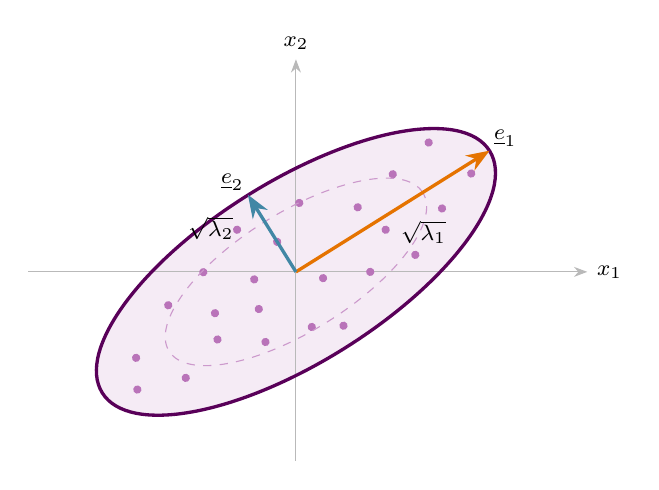
\begin{tikzpicture}[scale=1.0,>=Stealth]
\fill[violet!8, rotate=32] (0,0) ellipse (2.9 and 1.15);
\draw[->,gray!55] (-3.4,0) -- (3.7,0) node[right,black] {\footnotesize $x_1$};
\draw[->,gray!55] (0,-2.4) -- (0,2.7) node[above,black] {\footnotesize $x_2$};
% a scatter to show the ellipse is a contour of the data, not a bare curve
\begin{scope}[rotate=32]
  \foreach \p in {(-2.3,0.15),(-1.9,-0.4),(-1.6,0.5),(-1.3,-0.2),(-1.0,0.62),
                  (-0.8,-0.55),(-0.5,0.2),(-0.2,-0.7),(0.0,0.45),(0.25,-0.25),
                  (0.5,0.72),(0.8,-0.5),(1.1,0.28),(1.4,-0.62),(1.7,0.4),
                  (2.0,-0.3),(2.3,0.5),(-2.5,-0.2),(-0.35,0.85),(1.25,-0.15),
                  (0.15,-0.9),(-1.15,0.1),(2.55,-0.12),(-0.65,-0.15)}
    \fill[violet!55] \p circle (1.5pt);
\end{scope}
\draw[rotate=32,very thick,violet!70!black] (0,0) ellipse (2.9 and 1.15);
\draw[rotate=32,violet!40,dashed] (0,0) ellipse (1.9 and 0.75);
% principal axes
\draw[->,very thick,orange!90!black] (0,0) -- (2.46,1.54)
      node[above right,black,inner sep=1pt] {\footnotesize $\underline{e}_1$};
\draw[->,very thick,cyan!62!black] (0,0) -- (-0.61,0.98)
      node[above left,black,inner sep=1pt] {\footnotesize $\underline{e}_2$};
\node[black,inner sep=1pt] at (1.62,0.50)  {\footnotesize $\sqrt{\lambda_1}$};
\node[black,inner sep=1pt] at (-1.08,0.55) {\footnotesize $\sqrt{\lambda_2}$};
\end{tikzpicture}
\caption{Principal components in two dimensions. The ellipse is a contour of
constant Mahalanobis distance; its axes point along the eigenvectors
$\underline{e}_1$ and $\underline{e}_2$ of $\Sigma$, and their half-lengths are
proportional to $\sqrt{\lambda_1}$ and $\sqrt{\lambda_2}$. The analysis is a
rotation of the coordinate axes onto the axes of the ellipse: the correlation
between $x_1$ and $x_2$ that tilts the ellipse is exactly what the rotation
removes.}
\label{fig:pca}
\end{figure}

\subsection{How Much Variation Each Component Explains}

\begin{thm}[Total variation is preserved]
\label{thm:pcatrace}
$$\sum^{p}_{i=1}\operatorname{var}(X_i)
= \operatorname{tr}(\Sigma)
= \sum^{p}_{i=1}\lambda_i
= \sum^{p}_{i=1}\operatorname{var}(Y_i).$$
\end{thm}

\begin{proof}
$\operatorname{tr}(\Sigma) = \operatorname{tr}(P\Lambda P')
= \operatorname{tr}(\Lambda P'P) = \operatorname{tr}(\Lambda)
= \sum\lambda_i$, using the cyclic property of the trace from
Section~1.4 and $P'P=I$.
\end{proof}

\begin{defn}[Proportion explained]
The proportion of total variation explained by the $i$th component is
$$\frac{\lambda_i}{\lambda_1+\cdots+\lambda_p},$$
and by the first $k$ components,
$\left(\lambda_1+\cdots+\lambda_k\right)/\left(\lambda_1+\cdots+\lambda_p\right)$.
\end{defn}

\begin{note}
Theorem~\ref{thm:pcatrace} is what licenses the word ``explained''. The total
variability is a fixed quantity, $\operatorname{tr}(\Sigma)$, and the
eigenvalues partition it exactly. If the first two components account for
$0.9$ of that total, then a two-dimensional plot of $Y_1$ against $Y_2$
reproduces ninety percent of the variation in $p$ variables --- and, crucially,
one knows what has been lost.
\end{note}

\begin{thm}[Correlation between a component and a variable]
$$\operatorname{corr}\left(Y_i, X_k\right)
= \frac{e_{ik}\sqrt{\lambda_i}}{\sqrt{\sigma_{kk}}}.$$
\end{thm}

These correlations, often called \emph{loadings}, are how a component is
interpreted: a component correlating strongly with several variables is read as
whatever those variables have in common.

\subsection{Components from the Correlation Matrix}

Principal components are \emph{not} invariant under rescaling of the variables,
and this is the most common source of error in applying them.

\begin{note}
Suppose one variable is a length in millimetres and another a mass in
kilogrammes. The first has a numerically large variance purely because of its
units, so the first component will point almost entirely along it and the
analysis will have discovered nothing but the choice of scale. Re-expressing the
length in metres would give a completely different answer.

The remedy is to standardise: work with
$Z_k = \left(X_k-\mu_k\right)/\sqrt{\sigma_{kk}}$, whose covariance matrix is
the correlation matrix $\rho$. Components extracted from $\rho$ are unaffected
by the units, and $\operatorname{tr}(\rho)=p$, so the proportion explained by
the $i$th component is simply $\lambda_i/p$.

Components from $\Sigma$ and from $\rho$ are \emph{not} related in any simple
way --- one cannot be obtained from the other by rescaling. Which to use is a
decision that must be made and stated. Standardise unless the variables are
already in comparable units and their differing variances are themselves
meaningful.
\end{note}

\subsection{Sample Principal Components}

In practice $\Sigma$ is unknown and is replaced by the sample covariance matrix
$S$ of Section~3.3. Writing
$(\widehat{\lambda}_i, \widehat{\underline{e}}_i)$ for the eigenvalue--eigenvector
pairs of $S$, the $i$th \emph{sample principal component} of an observation
$\underline{x}_j$ is
$$y_{ji} = \widehat{\underline{e}}_i'\left(\underline{x}_j-\overline{\underline{x}}\right),$$
the centring being conventional so that the components have mean zero. Every
statement of the previous sections holds with $\Sigma,\lambda_i,\underline{e}_i$
replaced by $S,\widehat{\lambda}_i,\widehat{\underline{e}}_i$.

\begin{note}
Two practical points. The eigenvector is determined only up to sign: if
$\widehat{\underline{e}}_i$ maximises the variance then so does
$-\widehat{\underline{e}}_i$, so software may return either, and a component
that appears to have reversed between two analyses may not have changed at all.
And if $n\leq p$ then $S$ is singular, so at most $n-1$ eigenvalues are
non-zero and no more than that many components exist --- a real constraint when
variables outnumber observations.
\end{note}

\subsection{How Many Components to Keep}

There is no test that settles this, and the honest answer is that it is a
judgement informed by several partial criteria.

\begin{enumerate}
\item[(i)] \textbf{Cumulative proportion.} Retain enough components to reach a
stated proportion of the total variation, commonly $0.8$ or $0.9$.
\item[(ii)] \textbf{The scree plot.} Plot $\widehat{\lambda}_i$ against $i$ and
look for the elbow beyond which the eigenvalues fall away slowly and evenly;
retain the components above it.
\item[(iii)] \textbf{Kaiser's rule.} Working from the correlation matrix, retain
components with $\widehat{\lambda}_i>1$, on the ground that a component
explaining less than one variable's worth of variance has not earned its place.
\item[(iv)] \textbf{Interpretability.} A component that cannot be described in
the language of the subject is of limited use however much variance it carries.
\end{enumerate}

\begin{figure}[H]
\centering
\begin{tikzpicture}[xscale=0.85,yscale=0.62]
\draw[->] (0,0) -- (8.4,0) node[right] {\footnotesize component $i$};
\draw[->] (0,0) -- (0,5.2) node[above] {\footnotesize $\widehat{\lambda}_i$};
\foreach \x in {1,...,8} \draw (\x,0.09) -- (\x,-0.09) node[below] {\footnotesize $\x$};
\foreach \y in {1,2,3,4} \draw (0.09,\y) -- (-0.09,\y) node[left] {\footnotesize $\y$};
\draw[gray!55,dashed] (0,1) -- (8.3,1);
\draw[thick] plot coordinates {(1,4.4) (2,2.6) (3,0.85) (4,0.62) (5,0.48) (6,0.36) (7,0.26) (8,0.18)};
\foreach \p in {(1,4.4),(2,2.6),(3,0.85),(4,0.62),(5,0.48),(6,0.36),(7,0.26),(8,0.18)}
  \node[circle,fill,inner sep=1.1pt] at \p {};
\draw[<-] (3.25,1.35) -- (4.4,2.2) node[right] {\footnotesize elbow};
\node[right] at (6.35,1.25) {\footnotesize $\widehat{\lambda}=1$};
\end{tikzpicture}
\caption{A scree plot. The first two eigenvalues stand well clear and the rest
decline gently along a straight tail --- the ``scree'' of loose rubble at the
foot of a cliff, which is where the name comes from. Both the elbow and
Kaiser's rule point to retaining two components here, though the two criteria
need not always agree.}
\label{fig:scree}
\end{figure}

\begin{note}
Principal components are a description of the data, not a model of them. No
distributional assumption has been used anywhere in this section --- only that
$\Sigma$ exists --- so there is no likelihood, no standard error and no test
attached to any of it. Multivariate normality becomes relevant only when
inference about the $\lambda_i$ is wanted, and Section~5 is where that
assumption enters.

A second caution. The components are chosen to maximise variance, and variance
is not the same as importance. A direction along which the data barely vary may
nonetheless be the one that separates two groups, in which case the leading
components will conceal exactly the structure being sought. That is a job for
the discriminant analysis of Section~6, which maximises \emph{separation}
rather than variance, and the distinction between the two is worth keeping
firmly in view.
\end{note}

\subsection*{Practice Problems}

\begin{problem}
Let
$$\Sigma = \begin{pmatrix} 5 & 2\\ 2 & 2 \end{pmatrix}.$$
Find the principal components, their variances, and the proportion of total
variation explained by the first.
\emph{Where to start: solve $\left|\Sigma-\lambda I\right|=0$ for the
eigenvalues, then find a unit eigenvector for each.}
\end{problem}

\begin{solution}
The characteristic equation is
$(5-\lambda)(2-\lambda)-4 = \lambda^{2}-7\lambda+6 = 0$, giving
$\lambda_1 = 6$ and $\lambda_2 = 1$.

For $\lambda_1=6$: $(\Sigma-6I)\underline{e}=0$ gives $-e_1+2e_2=0$, so
$\underline{e}_1 \propto (2,1)'$ and, normalised,
$\underline{e}_1 = (2,1)'/\sqrt5$. Similarly
$\underline{e}_2 = (-1,2)'/\sqrt5$.

Hence $Y_1 = \left(2X_1+X_2\right)/\sqrt5$ with variance $6$, and
$Y_2 = \left(-X_1+2X_2\right)/\sqrt5$ with variance $1$. The first component
explains $6/(6+1) = 0.857$ of the total variation, and
$\operatorname{tr}(\Sigma) = 5+2 = 7 = \lambda_1+\lambda_2$ as
Theorem~\ref{thm:pcatrace} requires.
\end{solution}

\begin{problem}
For the same $\Sigma$, compute $\operatorname{corr}(Y_1,X_1)$ and
$\operatorname{corr}(Y_1,X_2)$, and interpret the first component.
\end{problem}

\begin{problem}
Show that if $\Sigma$ is diagonal then the principal components are the original
variables, in decreasing order of variance. Explain why this is the expected
answer.
\emph{Where to start: the eigenvectors of a diagonal matrix are the coordinate
axes.}
\end{problem}

\begin{problem}
Let $X_1$ be a length in centimetres and $X_2$ a mass in grams, with
$$\Sigma = \begin{pmatrix} 400 & 10\\ 10 & 4\end{pmatrix}.$$
Find the first principal component from $\Sigma$, then re-express $X_1$ in
metres and find it again. Comment on what the analysis has discovered in each
case, and repeat the exercise using the correlation matrix.
\end{problem}

\begin{solution}
From $\Sigma$ the first component is almost exactly $X_1$: the variance of $X_1$
is a hundred times that of $X_2$ purely because of its units, so
$\lambda_1\approx400$ with $\underline{e}_1\approx(1,0)'$. Re-expressing the
length in metres divides its variance by $10^{4}$, giving
$\Sigma^{*} = \begin{pmatrix}0.04 & 0.1\\ 0.1 & 4\end{pmatrix}$, and now the
first component lies almost along $X_2$. The two analyses disagree completely,
and neither has found anything but the choice of unit.

From the correlation matrix, $\rho = \begin{pmatrix}1 & 0.25\\ 0.25 & 1\end{pmatrix}$
in both cases, with $\lambda_1 = 1.25$, $\underline{e}_1 = (1,1)'/\sqrt2$, and
$\lambda_2 = 0.75$. The answer is now the same whichever units are used, and it
says something about the data rather than about the measuring instrument.
\end{solution}

\begin{problem}
Prove that $\prod^{p}_{i=1}\lambda_i = \left|\Sigma\right|$, and hence that the
generalised variance of Section~3.4 is the product of the component variances.
What does a zero eigenvalue imply about the variables?
\end{problem}

\begin{problem}
Explain why the sample principal components are unchanged if every observation
has a fixed vector $\underline{c}$ added to it, but change if each variable is
multiplied by a different constant.
\end{problem}

\begin{problem}
A scree plot of eight components shows eigenvalues
$4.4,\ 2.6,\ 0.85,\ 0.62,\ 0.48,\ 0.36,\ 0.26,\ 0.18$ obtained from a
correlation matrix. How many components would each of the four criteria of this
section retain? Where they disagree, say which you would follow and why.
\emph{Where to start: the eigenvalues sum to $p$; check that they do.}
\end{problem}

\begin{problem}
Give an example, or describe one, in which the first principal component
conceals the difference between two known groups. What does this show about
using principal components as a preliminary to classification?
\end{problem}


\section{The Multivariate Normal Distribution}

\subsection{Definition and Basic Properties}

The distribution this section is named after has been used implicitly since the
covariance matrices of Section~2; it is defined here, and the properties that
the inference of the following subsections relies on are established before
they are used.

\begin{defn}[Multivariate normal distribution]
A random vector $\underline{X} = (X_1,\dots,X_p)'$ has the \emph{multivariate
normal} distribution with mean $\underline{\mu}$ and covariance matrix $\Sigma$,
written $\underline{X}\sim N_p(\underline{\mu},\Sigma)$, if for
$\Sigma$ positive definite its density is
$$f(\underline{x}) = \frac{1}{(2\pi)^{p/2}\left|\Sigma\right|^{1/2}}
\exp\left\{-\tfrac{1}{2}\left(\underline{x}-\underline{\mu}\right)'
\Sigma^{-1}\left(\underline{x}-\underline{\mu}\right)\right\},
\qquad \underline{x}\in\mathbb{R}^{p}.$$
\end{defn}

\begin{note}
Compare the exponent with the univariate case, where it is
$-\left(x-\mu\right)^{2}/2\sigma^{2}$. The quadratic form
$\left(\underline{x}-\underline{\mu}\right)'\Sigma^{-1}
\left(\underline{x}-\underline{\mu}\right)$ is the squared Mahalanobis distance
of Section~1.9, so the density depends on $\underline{x}$ only through that
distance from the mean --- it is constant on the ellipsoids of Section~4, whose
axes are the eigenvectors of $\Sigma$ and whose extents are proportional to
$\sqrt{\lambda_i}$. The two constants have the same origin as in one dimension:
$\left|\Sigma\right|^{1/2}$ generalises $\sigma$, and $(2\pi)^{p/2}$ is the
normalising constant of $p$ independent standard normals.
\end{note}

\begin{thm}[Linear combinations]
\label{thm:mvnlinear}
If $\underline{X}\sim N_p(\underline{\mu},\Sigma)$ then for any
$A_{q\times p}$ and $\underline{b}_{q\times1}$ of constants,
$$A\underline{X}+\underline{b}\ \sim\
N_q\left(A\underline{\mu}+\underline{b},\ A\Sigma A'\right).$$
In particular every linear combination
$\underline{a}'\underline{X}$ is univariate normal.
\end{thm}

\begin{note}
Theorem~\ref{thm:mvnlinear} is the property that makes the multivariate normal
tractable, and it has a converse that is often taken as the definition:
$\underline{X}$ is multivariate normal precisely when $\underline{a}'\underline{X}$
is univariate normal for every fixed $\underline{a}$. That formulation has the
advantage of remaining meaningful when $\Sigma$ is singular, where no density
exists --- the distribution then lives on a lower-dimensional subspace, which is
exactly the situation met in Section~4 when an eigenvalue is zero.
\end{note}

\begin{thm}[Marginals and independence]
\label{thm:mvnmarg}
Partition $\underline{X} = \begin{pmatrix}\underline{X}_1\\ \underline{X}_2\end{pmatrix}$
conformably with
$\underline{\mu} = \begin{pmatrix}\underline{\mu}_1\\ \underline{\mu}_2\end{pmatrix}$
and
$\Sigma = \begin{pmatrix}\Sigma_{11} & \Sigma_{12}\\ \Sigma_{21} & \Sigma_{22}\end{pmatrix}$.
Then
\begin{enumerate}
\item[(i)] $\underline{X}_1 \sim N_{q}\left(\underline{\mu}_1,\Sigma_{11}\right)$;
\item[(ii)] $\underline{X}_1$ and $\underline{X}_2$ are independent if and only
if $\Sigma_{12}=0$.
\end{enumerate}
\end{thm}

\begin{note}
Part (ii) deserves emphasis because it is false in general. Zero covariance does
not imply independence for arbitrary distributions --- it says only that no
\emph{linear} association is present. Under joint normality the two coincide,
and this equivalence is used constantly in what follows. It requires
\emph{joint} normality: two variables that are each normal but not jointly so
can be uncorrelated and dependent.
\end{note}

\begin{thm}[Conditional distributions]
\label{thm:mvncond}
With the partition above and $\Sigma_{22}$ non-singular,
$$\underline{X}_1 \mid \underline{X}_2 = \underline{x}_2\ \sim\
N_q\left(\underline{\mu}_1 + \Sigma_{12}\Sigma_{22}^{-1}
\left(\underline{x}_2-\underline{\mu}_2\right),\ \
\Sigma_{11}-\Sigma_{12}\Sigma_{22}^{-1}\Sigma_{21}\right).$$
\end{thm}

\begin{note}
Two features of Theorem~\ref{thm:mvncond} are worth naming. The conditional mean
is a \emph{linear} function of $\underline{x}_2$ --- which is where the linear
regression of Section~8 comes from, the regression coefficients being
$\Sigma_{12}\Sigma_{22}^{-1}$. And the conditional covariance does not depend on
$\underline{x}_2$ at all: the conditional variability is the same wherever one
conditions, which is the multivariate statement of homoscedasticity. Both are
special properties of the normal and neither holds in general.

The matrix $\Sigma_{11}-\Sigma_{12}\Sigma_{22}^{-1}\Sigma_{21}$ is the Schur
complement of $\Sigma_{22}$, and it is never larger than $\Sigma_{11}$ in the
positive-definite ordering: conditioning on information cannot increase
uncertainty.
\end{note}

\begin{thm}[The quadratic form]
\label{thm:mvnchisq}
If $\underline{X}\sim N_p(\underline{\mu},\Sigma)$ with $\Sigma$ non-singular,
then
$$\left(\underline{X}-\underline{\mu}\right)'\Sigma^{-1}
\left(\underline{X}-\underline{\mu}\right)\ \sim\ \chi^{2}_{p}.$$
\end{thm}

\begin{proof}
By Section~1.9 write $\Sigma^{-1/2}$ for the symmetric square root and put
$\underline{Z} = \Sigma^{-1/2}\left(\underline{X}-\underline{\mu}\right)$. By
Theorem~\ref{thm:mvnlinear}, $\underline{Z}\sim N_p(\underline{0}, I)$, so its
components are independent standard normals, and the quadratic form equals
$\underline{Z}'\underline{Z} = \sum^{p}_{i=1}Z_i^{2}$, a sum of $p$ independent
squared standard normals.
\end{proof}

\begin{note}
Theorem~\ref{thm:mvnchisq} is what makes the confidence regions of the following
subsections ellipsoids rather than boxes. The set of $\underline{x}$ with
Mahalanobis distance below the $\chi^{2}_{p}$ critical value is an ellipsoid
centred at $\underline{\mu}$, oriented along the eigenvectors of $\Sigma$; it is
also the natural region for detecting outliers, since a point may be
unremarkable in each coordinate separately and far away in the joint sense.
\end{note}

\subsection{Sampling from a Multivariate Normal Population}

Let $\underline{X}_1,\dots,\underline{X}_n$ be a random sample from
$N_p(\underline{\mu},\Sigma)$, with
$\overline{\underline{X}} = \frac{1}{n}\sum\underline{X}_j$ and
$S = \frac{1}{n-1}\sum\left(\underline{X}_j-\overline{\underline{X}}\right)
\left(\underline{X}_j-\overline{\underline{X}}\right)'$.

\begin{thm}[Maximum likelihood estimators]
The maximum likelihood estimators of $\underline{\mu}$ and $\Sigma$ are
$$\widehat{\underline{\mu}} = \overline{\underline{X}},
\qquad
\widehat{\Sigma} = \frac{1}{n}\sum^{n}_{j=1}
\left(\underline{X}_j-\overline{\underline{X}}\right)
\left(\underline{X}_j-\overline{\underline{X}}\right)'
= \frac{n-1}{n}\,S .$$
\end{thm}

\begin{note}
As in the univariate case the maximum likelihood estimator of the covariance
divides by $n$ and is biased; $S$ divides by $n-1$ and is unbiased. Both are
used, and which is meant should always be checked, particularly in software
output.
\end{note}

\begin{thm}[Sampling distributions]
\label{thm:sampling}
For a random sample from $N_p(\underline{\mu},\Sigma)$:
\begin{enumerate}
\item[(i)] $\overline{\underline{X}}\ \sim\ N_p\!\left(\underline{\mu},\ \tfrac{1}{n}\Sigma\right)$;
\item[(ii)] $(n-1)S \sim W_p\left(n-1,\Sigma\right)$, the Wishart distribution
defined below;
\item[(iii)] $\overline{\underline{X}}$ and $S$ are independent.
\end{enumerate}
\end{thm}

\begin{note}
These are the exact multivariate analogues of the univariate facts that
$\overline{X}\sim N(\mu,\sigma^{2}/n)$, that $(n-1)s^{2}/\sigma^{2}\sim\chi^{2}_{n-1}$,
and that the two are independent. Part (iii) is the property that makes
Hotelling's $T^{2}$ possible at all: the statistic is a ratio involving both
$\overline{\underline{X}}$ and $S$, and its distribution can only be derived
because the numerator and denominator are independent.
\end{note}

\subsection{The Wishart Distribution}

The chi-square distribution describes the sampling behaviour of a sample
variance. Its multivariate counterpart describes the sampling behaviour of a
whole covariance matrix, and it is the distribution behind every result in the
remainder of this section.

\begin{defn}[Wishart distribution]
Let $\underline{Z}_1,\dots,\underline{Z}_m$ be independent
$N_p(\underline{0},\Sigma)$ vectors. The distribution of the random matrix
$$W = \sum^{m}_{j=1}\underline{Z}_j\underline{Z}_j'$$
is the \emph{Wishart distribution} with $m$ degrees of freedom and scale matrix
$\Sigma$, written $W\sim W_p(m,\Sigma)$.
\end{defn}

\begin{note}
Taking $p=1$ and $\Sigma=\sigma^{2}$ gives $W = \sum Z_j^{2}$ with the $Z_j$
independent $N(0,\sigma^{2})$, so $W/\sigma^{2}\sim\chi^{2}_{m}$: the Wishart
with $p=1$ \emph{is} the chi-square, scaled. Everything in this subsection
reduces to a familiar univariate statement when $p=1$, and checking that it does
is the quickest way to remember any of it.
\end{note}

\begin{thm}[Properties]
\label{thm:wishart}
Let $W\sim W_p(m,\Sigma)$ and $W_1, W_2$ be independent Wisharts with the same
scale matrix. Then
\begin{enumerate}
\item[(i)] $E(W) = m\Sigma$;
\item[(ii)] $W_1 + W_2 \sim W_p\left(m_1+m_2,\Sigma\right)$;
\item[(iii)] $AWA' \sim W_q\left(m, A\Sigma A'\right)$ for $A_{q\times p}$ of constants;
\item[(iv)] $W$ is positive definite with probability one if and only if
$m\geq p$.
\end{enumerate}
\end{thm}

\begin{note}
Part (iv) is a practical constraint rather than a technicality. Since
$(n-1)S\sim W_p(n-1,\Sigma)$, the sample covariance matrix is singular whenever
$n-1<p$ --- fewer observations than variables --- and then $S^{-1}$ does not
exist. Every procedure in the rest of this section requires $S^{-1}$, so all of
them fail in that regime, which is the formal reason a multivariate analysis
needs more observations than variables. It is the same fact met in
Section~4.4, where at most $n-1$ principal components can be extracted.
\end{note}

\begin{note}
Part (i) explains the divisor in $S$: since $E\left[(n-1)S\right] = (n-1)\Sigma$
we have $E(S)=\Sigma$, so dividing the sum of squares and cross-products by
$n-1$ rather than $n$ is what makes $S$ unbiased --- the same reason as in one
dimension, with the same degrees of freedom lost to estimating the mean.
\end{note}

\begin{note}
With this in place, Hotelling's $T^{2}$ of the next subsection can be seen for
what it is. The univariate $t$ statistic squares to
$$t^{2} = \frac{\left(\overline{X}-\mu\right)^{2}}{s^{2}/n}
= n\left(\overline{X}-\mu\right)\left(s^{2}\right)^{-1}\left(\overline{X}-\mu\right),$$
and replacing the scalars by their matrix counterparts gives
$$T^{2} = n\left(\overline{\underline{X}}-\underline{\mu}\right)'
S^{-1}\left(\overline{\underline{X}}-\underline{\mu}\right).$$
It is a normal vector and an independent Wishart matrix combined exactly as a
normal variable and an independent chi-square are combined in the univariate
case, which is why its null distribution is a multiple of an $F$.
\end{note}


\subsection{Hotellings}
\pagebreak






\subsection{Wilks Lambda}
The Hotellings $T^2$ statistics was argued using its analogue $t^2$  of students $t$. One common procedure for constructing test procedures is called the likelihood ratio method.\\

From our previous work we noted that the maximum of the multivariate normal likelihood has $\underline{\mu}$ and $\Sigma$ are varied over other possible values is give by 
\begin{equation}\tag{1}
\max\limits_{\mu, \Sigma} L\big(\underline{\mu},\Sigma\big) = \big(2\pi\big)^{-np/2}\big|\widehat{\Sigma}\big|^{\frac{n}{p}}e^{-np/2}
\end{equation} where $\displaystyle{\widehat{\Sigma}=\frac{1}{n}\sum^n_{j=1}\big(\underline{X}_j-\overline{\underline{X}}\big)\big(\underline{X}_j-\overline{\underline{X}}\big)'}$ and $\displaystyle{\widehat{\mu}=\overline{X}=\frac{1}{n}\sum^n_{j=1}\underline{X}_j}$ are the maximu likelihood estimates.\\

Recall that the maximum likelihood estimates of $\widehat{\mu}$ and $\widehat{\Sigma}$ are those choices for $\underline{\mu}$ and $\Sigma$  that best explains the observed values for the random sample under the hypothesis $H_0:\underline{\mu} = \underline{\mu}_0$ the normal likelihood becomes
\begin{equation}\tag{2}
L\big(\mu_0,\Sigma\big)= \big(2\pi\big)^{-np/2}\big|\Sigma\big|^{-n/2}\exp\Big\{-\frac{1}{2}\sum^n_{j=1}\big(\underline{X}_j-\underline{\mu}_0\big)'\Sigma^{-1}\big(\underline{X}_j-\underline{\mu}_0\big)\Big\}
\end{equation}


The mean $\underline{\mu}_0$ is fixed since it is known, but $\Sigma$ can be varied to find the value that most likely with the given data. The value is obtained by maximizing $L\big(\mu_0,\Sigma\big)$ to with respect to $\Sigma$.\\
Using the steps of maximization carried we have
\begin{align*}
-\frac{1}{2}\sum^n_{j=1}\big(\underline{X}_j-\underline{\mu}_0\big)'\Sigma^{-1}\big(\underline{X}_j-\underline{\mu}_0\big) & = -\frac{1}{2}\sum^n_{j=1}tra\Big\{\Sigma^{-1}\big(\underline{X}_j-\underline{\mu}_0\big)\big(\underline{X}_j-\underline{\mu}\big)'\Big\}\\
& = -\frac{1}{2}tra\Big\{\Sigma^{-1}\Big(\sum^n_{j=1}\big(\underline{X}_j-\underline{\mu}_0\big)\big(\underline{X}_j-\underline{\mu}_0\big)'\Big)\Big\}\\
\end{align*}


Applying one results and \,$\displaystyle{B= \sum^n_{j=1}\big(\underline{X}_j-\underline{\mu}_0\big)\big(\underline{X}_j-\underline{\mu}_0\big)'}\,$ and $b= \frac{n}{2}$ we have 

$$\max\limits_{\Sigma}L\big(\mu_0,\Sigma\big) = \frac{1}{(2\pi)^{np/2}\big|\widehat{\Sigma}_0\big|^{n/2}}e^{-np/2}\quad \cdots\cdot\cdots\quad  (3)$$
with\, $\displaystyle{\widehat{\Sigma}_0=\frac{1}{n}\sum^n_{j=1}\big(\underline{X}_j-\underline{\mu}_0\big)\big(\underline{X}_j-\underline{\mu}_0\big)'}$.\\

To determine whether $\Sigma_0$ is plausible value for $\underline{\mu}$ the $\max L\big(\mu_0,\Sigma\big)$ is compared with unrestricted maximum $L\big(\underline{\mu},\Sigma\big)$. The resulting ratio is called the likelihood ratio statistic. Using (1) and (3) we have likelihood ratio $\Delta$



\begin{equation}\tag{4}
\Delta = \frac{\max\limits_{\Sigma}L\big(\underline{\mu}_0,\Sigma\big)}{\max\limits_{\underline{\mu},\Sigma}L\big(\underline{\mu},\Sigma\big)}=\Bigg(\frac{\big|\hat{\Sigma}\big|}{\big|\hat{\Sigma_0}\big|}\Bigg)^{\frac{n}{2}}
\end{equation}


The equivalent statistic is $\Delta^{2/n} = \frac{\big|\widehat{\Sigma}\big|}{\big|\widehat{\Sigma_0}\big|}\qquad (5)$ is called Wilks Lambda.\\\\\\\\






\pagebreak
\begin{note}
\begin{enumerate}
\item If the observed value of the likelihood ratio is too small, the hypothesis $H_0: \underline{\mu} = \underline{\mu}_0$ is unlikely to be true and is, therefore, rejected.

\item $\displaystyle{\Delta = \Bigg(\frac{\big|\widehat{\Sigma}\big|}{\big|\widehat{\Sigma}_0\big|}\Bigg)^{\frac{n}{2}}=\Bigg(\frac{\Big|\sum\limits_{j=1}^n\big(\underline{X}_j-\overline{\underline{X}}\big)\big(\underline{X}_j-\overline{\underline{X}}\big)'\Big|}{\Big|\sum\limits_{j=1}^n\big(\underline{X}_j-\underline{\mu}_0\big)\big(\underline{X}_j-\underline{\mu}_0\big)'\Big|}\Bigg)}$

where $C_{\alpha}$ is the lower $(100\alpha)\%$ of percentile of the distribution of $\Delta$.





\item It can be shown that 
\begin{align*}
\Delta_w & = \Delta^{2/n}= \Bigg(1 + \frac{T^2}{n-1}\Bigg)^{-1}\\
& = \frac{\big|\widehat{\Sigma}\big|}{\big|\widehat{\Sigma}_0\big|}\\
\end{align*}


\begin{equation}\tag{7}
\text{or}\quad  T^2 = (n-1)\frac{\big|\widehat{\Sigma}\big|}{\big|\widehat{\Sigma}_0\big|}-(n-1)
\end{equation}\\



\item Suppose that which to find \,$\displaystyle{ \Delta_{w,\alpha} = C_{\alpha} \ni Pr\big(\Delta_w < \Delta_{\alpha}\big) = \alpha}$\\

How do we proceed?
\begin{align*}
Pr\big(\Delta_w<C_{\alpha}\big) & = Pr\Bigg(\Bigg(1 + \frac{T^2}{n-1}\Bigg)^{-1}<C_{\alpha}\Bigg)\\\\
                                & = Pr\Bigg(\frac{1}{C_{\alpha}}<1 + \frac{T^2}{n-1}\Bigg)\\
\end{align*}


$$Pr\Bigg(\Bigg(\frac{1}{C_{\alpha}}-1\Bigg)(n-1)<T^2\Bigg)$$\\



$$Pr\Bigg(\Bigg(\frac{1-C_{\alpha}}{C_{\alpha}}\Bigg)(n-1)<\frac{(n-1)p}{n-p}F_{p,n-p}\Bigg)$$\\


$$Pr\Bigg(\Bigg(\frac{1-C_{\alpha}}{C_{\alpha}}\Bigg)\frac{n-p}{p}<F_{p,n-p}\Bigg)<\alpha$$\\

$$\implies\quad  F_{p,n-p,\alpha}=\frac{\big(1-C_{\alpha}\big)}{C_{\alpha}}\frac{(n-p)}{p}$$

$$\text{make}\quad  C_{\alpha}\qquad \text{the subject}$$

$$C_{\alpha} = \frac{n-p}{n-p+pF_{p,n-p,\alpha}}$$\\
\end{enumerate}
\end{note}











\begin{exa}
Consider the ventilation value in the handout the $F$ value calculated using SAS is given as 2.9276\\
To calculate the $T^2$ we observe that 
$$p=t-1,  n =8,  t=6 $$
\end{exa}

\begin{align*}
T^2 & = \frac{(n-1)p}{n-p}F_{p,n-p,\alpha}\\
& = \frac{(n-1)(t-1)}{n-(t-1)}\times 2.9276\\
& = \frac{7\times 5}{8-6+1}\times 2.9276\\
& = \frac{35}{3}\times 2.9276 = 34.155
\end{align*}
 is the observed value of Hotellings.\\
 
$-$ The critical value is obtained in the similarly manner
$$ F_{5,3,\alpha}=F_{5,3,0.05}=9.01$$

$$T^2_{0.05}= \frac{35}{3}\times 9.01=105.12$$

$-$ Since $T^2_{obse} = 34.155< T^2_{critical} =105.12$
We fail to reject $H_0$ and conclude that there is not enough evidence evidence to suggest that ventilation volume is affected by temperature.\\\\














\pagebreak
\subsection{Confidence Regions}
\begin{enumerate}
\item Here we extended the concept of the unvariate confidence interval to a multivariate confidence region.
\item The region is determined by the data and for the moment, denotes it by $R(X)$, where $X=
\begin{pmatrix}
\underline{X}_1,\underline{X}_2,\ldots,\underline{X}_n\\
\end{pmatrix}$is the data matrix.
\item The region $R(X)$ is said to the $100(1-\alpha)\%$ confidence region if before the sample is selected.\\

$Pr( R(X)$ will cover the true $\underline{\theta})=1-\alpha \qquad (1)$
\item This $Pr$ is calculated under  the true but unknown value of $\theta$.
\item The confidence region for $\underline{\mu}$ of $P-$ dimensional normal population from our previous work satisfies.
\begin{equation}\tag{2}
Pr\Bigg[n\big(\overline{\underline{X}}-\underline{\mu}\big)'S^{-1}\big(\overline{\underline{X}}-\underline{\mu}\big)\leq \frac{(n-1)p}{n-p}F_{p,n-p}(\alpha)\Bigg] = 1 - \alpha
\end{equation}
\item For a particular sample $\overline{\underline{X}}$ and $S$ can be computed and the inequality 
$$ n\big(\overline{\underline{X}}-\underline{\mu}\big)'S^{-1}\big(\overline{\underline{X}}-\underline{\mu}\big)\leq \frac{(n-1)p}{n-p}F_{p,n-p}(\alpha)$$ 
will define a region $R(X)$ and this particular region is an ellipsoid centered at $\overline{\underline{X}}$.\\\\
\end{enumerate}








\begin{defn}
A $100(1-\alpha)\%$ confidence region for the mean of $p-$ dimensional normal distribution is the set determined by all $\underline{\mu}$ such that $$n\big(\overline{\underline{X}}-\underline{\mu}\big)'S^{-1}\big(\overline{\underline{X}}-\underline{\mu}\big)\leq \frac{p(n-1)}{n-p}F_{p,n-p,1-\alpha}$$
where $\overline{\underline{X}}$ and $S$ are the usual sample quantities.\\
\end{defn}

Beginning at the center $\overline{\underline{X}}$ the axes of the confidence ellipsoid are $$\pm \sqrt{\lambda_i}\sqrt{\frac{p(n-1)}{n(n-p)}F_{p,n-p,(1-\alpha)}}\underline{e}_i$$ where $S\underline{e}_i = \lambda_i\underline{e}_ip,  i= (1)p$.\\\\



\subsubsection*{Simultaneous Confidence Statements}
The confidence region in (3) 
\,$\displaystyle{ n\big(\overline{\underline{X}}-\underline{\mu}\big)'S^{-1}\big(\overline{\underline{X}}-\underline{\mu}\big) \leq C^2}\,$ where $C$ is constant. Correctly asses the joint knowledge concern values for $\underline{\mu}$. There is need, however to make statements about the individual components means or specific linear combinations.\\

Let $\underline{X}\thicksim N_p\big(\underline{\mu},\Sigma\big)$ and consider the linear combinations. \begin{equation}\tag{4}
Z = L_1X_1 + L_2X_2 + \cdots+ L_pX_p
\end{equation}
From the previous work, we know that \begin{equation}\tag{5}
\mu_Z =E(Z) = E\big(\underline{L}'\underline{X}\big) = \underline{L}'E(\underline{X})=L'\underline{\mu}
\end{equation} and $\, \displaystyle{var(Z) = var\big(\underline{L}'\underline{X}\big) = \underline{L}'var(\underline{X})\underline{L}=\underline{L}'\Sigma\underline{L}\qquad (6)}$\\

Since $Z$ is a linear combination of normal variance, $Z$ itself has a normal distribution. \begin{equation}\tag{7}
Z\thicksim N\big(\underline{L}'\underline{\mu}, \underline{L}'\Sigma\underline{L}\big)
\end{equation} 

Once sample values are available, we can estimate $\mu_Z= \underline{L}'\underline{\mu}$ and $\Sigma_Z = \underline{L}'\Sigma \underline{L}$ in that case sample estimate become \begin{equation}\tag{8}
\overline{Z} = \underline{L}'\overline{\underline{X}}
\end{equation}
$S^2_2 = \displaystyle{\underline{L}'S\underline{L}}$, where $S$ is the usual sample covariance matrix.\\

For the fixed $L$, and $\sigma^2_Z$ unknown  a $100(1-\alpha)\%$ confidence interval for $\mu_Z = \underline{L}'\underline{\mu}$ based on student's $t$ ratio
\begin{equation}\tag{9}
t = \frac{\overline{Z}-\mu_Z}{S_Z/\sqrt{n}}=\frac{\sqrt{n}\big(\underline{L}'\overline{\underline{X}}-\underline{L}'\underline{\mu}\big)}{\sqrt{\underline{L}'S\underline{L}}}
\end{equation}
and leads to the statement $M.E=$ Margin of Error

$$\overline{Z}-t_{n-1,(1-\alpha/2)}\cdot \frac{S_Z}{\sqrt{n}}\leq \mu_Z \leq \overline{Z}+t_{n-1,(1-\alpha/2}\cdot \frac{S_Z}{\sqrt{n}}$$

or 

\begin{equation}\tag{10}
\underline{L}'\overline{\underline{X}}-t_{n-1, (1-\alpha/2)} \sqrt{\frac{\underline{L}'S\underline{L}}{n}} \leq L'\mu \leq \underline{L}'\overline{\underline{X}} + t_{n-1,(1-\alpha/2)}\frac{\sqrt{\underline{L}'S\underline{L}'}}{\sqrt{n}}
\end{equation}\\\\



\begin{center}
\textbf{The $T^2-$ Confidence Intervals}
\end{center}
It can be shown that $T^2=n\big(\overline{\underline{X}}-\underline{\mu}\big)'S^{-1}\big(\overline{\underline{X}}-\underline{\mu}\big)\leq C^2$ implies that $\frac{n\big(L'\overline{\underline{X}}-L'\underline{\mu}\big)^2}{L'SL}\leq C^2\quad  \forall L$ or 
$$L'\overline{\underline{X}}-C\sqrt{\frac{L'SL}{n}}\leq \underline{L}'\underline{\mu}\leq L'\underline{\overline{X}}+C\sqrt{\frac{L'SL}{n}}\quad  \cdots\quad (*)$$

and choosing $C^2= \frac{p(n-1)}{n-p}F_{p,n-p}(1-\alpha)$, then the interval \begin{equation}\tag{11}
L'\overline{\underline{X}}- \sqrt{\frac{p(n-1)}{n-p}F_{p,n-p,(1-\alpha)}\frac{L'SL}{n}}\leq \underline{L}'\underline{\mu}\leq L'\overline{\underline{X}}+\sqrt{\frac{p(n-1)}{n-p}F_{p,n-p,(1-\alpha)}\frac{L'SL}{n}}
\end{equation}
a $100(1-\alpha)\%$ interval in (11) may be refereed as $T$ interval since coverage probability for various choices may be determined by the Hotelling's $T^2$ distribution associated with $F$ distribution.\\\\



\begin{center}
\textbf{Individual Mean Confidence Intervals}
\end{center}
Various choices of $L$ lead to intervals of individual component means
\begin{align*}
L'_1 & = 
\begin{pmatrix}
1, & 0, & 0, & \cdots& 0\\
\end{pmatrix}\\
L'_2 & = \begin{pmatrix}
0, & 1, & 0, & \cdots& 0\\
\end{pmatrix}\\
\vdots & \\
L'_p & = \begin{pmatrix}
0, & 0, & 0, & \cdots& 1\\
\end{pmatrix}\\
\end{align*}



\begin{align*}
L_1 & : \overline{X}_1-\sqrt{\frac{p(n-1)}{n-p}F_{p,n-p,1-\alpha}\frac{S_{11}}{n}}\leq \mu_1\leq \overline{X}_1+ \sqrt{\frac{p(n-1)}{n-p}F_{p,n-p,1-\alpha}\frac{S_{11}}{n}}\\\\
L_2 & : \overline{X}_2-\sqrt{\frac{p(n-1)}{n-p}F_{p,n-p,1-\alpha}\frac{S_{22}}{n}}\leq \mu_2\leq \overline{X}_2+ \sqrt{\frac{p(n-1)}{n-p}F_{p,n-p,1-\alpha}\frac{S_{22}}{n}}\\
& \vdots \\
& \vdots \\
L_p & : \overline{X}_p-\sqrt{\frac{p(n-1)}{n-p}F_{p,n-p,1-\alpha}\frac{S_{pp}}{n}}\leq \mu_2\leq \overline{X}_2+ \sqrt{\frac{p(n-1)}{n-p}F_{p,n-p,1-\alpha}\frac{S_{pp}}{n}}\\
\end{align*}



\begin{exa}
Consider the layout showing the performance of students in three assignments in some statistical course in the accordance of year 200 semester 1\\
\end{exa}

\textbf{Data}\\
$X_1=$ score out of 100 in assignment 1\\
$X_2=$ score out of 100 in assignment 2\\
$X_3=$ score out of 100 in assignment 3\\

This is an example of a repeated measurements design in which each has three measurements.\\

Let $\underline{\mu}=\begin{pmatrix}
\mu_1, & \mu_2, & \mu_3\\
\end{pmatrix}'$ and assume that $\underline{X}_i\thicksim N_3\big(\underline{\mu},\Sigma\big)$ where $\underline{X}_i$ is a vector of scores for the $i^{\text{th}}$ student

\begin{enumerate}
\item Test $H_0:\mu_1 = \mu_2 = \mu_2$ vs $H_a: \mu_i\neq \mu_j$ for some $i\neq j$.
\item Find a $95\%$ confidence region for the true mean vector $\underline{\mu}=\begin{pmatrix}
\mu_1\\ \mu_2\\ \mu_3\\
\end{pmatrix}
$
\item Find a $95\%$ confidence interval for $\mu = \frac{1}{3}\big(\mu_1+\mu_2+\mu_3\big)$.
\item Find a $95\%$ C.I for $\mu_1$, $\mu_2$ and $\mu_3$ respectively.
\item Determine whether $\mu_0 = \begin{pmatrix}
50, & 50, & 50\\
\end{pmatrix}$.\\
\end{enumerate}



\begin{solution}
Data
$$\overline{X}=\begin{pmatrix}
76.44\\ 
69.75\\
68.06\\
\end{pmatrix}
\qquad 
S = 
\begin{pmatrix}
55.739 & -7.964 & -12.844\\
       &  422.879 & 29.929\\
       &          & 147.597\\
\end{pmatrix}
$$\\
\end{solution}

$$S^{-1} = \begin{pmatrix}
0.0183304 & & \\
0.02359   & 0.0024021 & \\
0.0015441 & 0.0004656 & 0.0069898\\   
\end{pmatrix}$$\\

$$n=36,  t=p=3$$



\begin{enumerate}
\item 
\begin{enumerate}
     \item[$-$] $H_0: \mu_1 = \mu_2 = \mu_3$ vs $H_a: \mu_i \neq \mu_j$ for some $i\neq j$.
     
     \item[$-$] Test $$T^2=n\big(C\overline{X}\big)'\big(CSC'\big)^{-1}\big(C\overline{X}\big)$$
          
     $$C=\begin{pmatrix}
     1 & -1 & 0\\
     0 & 1 & -1\\
     \end{pmatrix}$$
     
     \item[$-$] Decision:\\
     Reject $H_0$ if $F_{obs}>F_{2,34,0.95}=3.275$
     
     \item[$-$] Conclusion: 
      $$T^2 = 11.657772$$
      
 \begin{align*}
 F_{obs} & = \frac{n-C}{(n-1)C}T^2\qquad  C- \text{number of rows in the matrix } C\\
         & = \frac{36-2}{(36-1)2}(11.657772)\\
         & = 5.662
 \end{align*}
Since $F_{obs} > 3.275$ we reject $H_0$ and conclude that the 3 means are not equal. In other terms the average performance in the three assignments are different.\\\\
\begin{problem}
verify $T^2$\\
\end{problem}
\end{enumerate}

\item The $95\%$ confidence region is give by $$ n\big(\overline{X}-\underline{\mu}\big)'S^{-1}\big(\overline{X}-\underline{\mu}\big) \leq \frac{p(n-1)}{n-p}F_{p,n-p}(1-\alpha)$$\\

\begin{align*}
F_{3,36-3}(0.95) & = F_{3,33}(0.95)\\
                 & = \frac{1}{2}(2.92+2.84)\\
                 & = 2.88\\
\end{align*}

$$\frac{p(n-1)}{n-p}F_{3,33}(0.95) = \frac{3\times 35}{33}\times 2.88= 9.164$$\\



$$\overline{\underline{X}}-\underline{\mu} = \begin{pmatrix}
76.44 - \mu_1\\
69.75 - \mu_2\\
68.06 - \mu_3\\
\end{pmatrix} $$\\



$$36
\begin{pmatrix}
76.44 - \mu_1\\
69.75 - \mu_2\\
68.06 - \mu_3\\
\end{pmatrix}'
\begin{pmatrix}
0.0183304 &  & \\
0.0002359 & 0.002401 & \\
0.0015441 & 0.004646 & 0.06989\\
\end{pmatrix}
\begin{pmatrix}
76.44 - \mu_1\\
69.75 - \mu_2\\
68.06 - \mu_3\\
\end{pmatrix} 
\leq 9.164
$$ 
expanding may give the general formula $$a\mu^2_1 + b \mu^2_2 + c\mu^2_3 + d\mu_1\mu_2 + e\mu_1\mu_3 + f\mu_2\mu_3 + g \leq 9.164$$\\

\item Let us find the $T^2$ Hotelling interval
$$L'\overline{\underline{X}} = \begin{pmatrix}
\frac{1}{3}, & \frac{1}{3}, & \frac{1}{3}\\
\end{pmatrix}
\begin{pmatrix}
76.44\\ 69.75\\ 68.00\\
\end{pmatrix}
= 71.42\\
$$


\begin{align*}
L'SL & = \begin{pmatrix}
\frac{1}{3}, & \frac{1}{3}, & \frac{1}{3}\\
\end{pmatrix}
\begin{pmatrix}
55.739 & -7.964 & -12.844\\
       &  422.879 & 29.929\\
       &          & 147.597\\
\end{pmatrix}
 \begin{pmatrix}
\frac{1}{3}\\\\ \frac{1}{3} \\\\ \frac{1}{3}\\
\end{pmatrix}\\
& = \frac{1}{9}\begin{pmatrix}
34.931, & 444.844, & 164.982\\
\end{pmatrix}
\begin{pmatrix}
1\\ 1\\ 1\\
\end{pmatrix}\\
& = \frac{1}{9}(644.757) = 71.637\\
\end{align*}
The $T^2$ interval is 
\begin{align*}
L'\overline{\underline{X}} \pm \sqrt{\frac{p(n-1)}{n-p}F_{p,n-p}(1-\alpha)\frac{L'SL}{n}} & = 71.42 \pm \sqrt{\frac{9.164\times 71.6397}{36}}\\
& = 71.42 \pm 4.27\\
& = (67.15, 75.69)\\
\end{align*}


 The $95\%$ confidence interval for students $t$ is
 $$t_{n-1,(1-\alpha/2)} = t_{35,0.975} = 2.03$$
 
\begin{align*}
 L'\overline{\underline{X}} & \pm t_{n-1,(1-\alpha/2)}\sqrt{\frac{L'SL}{n}}\\\\
 71.42 & \pm 2.03 \sqrt{\frac{71.6397}{36}}\\\\
 71.42 & \pm 2.03 \times 1.41067\\
 71.42 & \pm 2.864\\
 & = (68.56, 74.28)
\end{align*}
The $T^2$ seems to be more conservative than the students $t$.\\


\item Individual confidence intervals
\begin{align*}
\mu_1: & \overline{X}_1 \pm \sqrt{\frac{p(n-1)}{n-p}F_{p,n-p}(1-\alpha)\frac{S_{11}}{n}}\\\\
      & 76.44 \pm \sqrt{9.164 \times \frac{55.739}{36}}\\
      & = 76.44 \pm \sqrt{14.1887}\\
      & = 76.44 \pm 3.77\\
      & \equiv (67.67, 75.21)\\ 
\end{align*}


\begin{align*}
\mu_2 : & \overline{X}_2 \pm \sqrt{9.164 \times \frac{S_{22}}{n}}\\\\
& 69.75 \pm \sqrt{9.164 \times \frac{422.879}{36}}\\
& = 69.75\pm 10.38\\
& \equiv (59.37, 80.13)\\
\end{align*}

\begin{align*}
\mu_3 :& 68.06 \pm \sqrt{9.164 \times \frac{147.597}{36}}\\
 & = 68.06 \pm \\
 & \equiv (61.93, 74.19)\\
\end{align*}


\item $\big(\overline{\underline{X}}-\underline{\mu}\big)'= \begin{pmatrix}
26.44, & 19.75, & 18.06\\
\end{pmatrix}
$ we refer to 
\begin{align*}
n\big(\overline{\underline{X}}-\underline{\mu}_0\big)'S^{-1}\big(\overline{\underline{X}}-\underline{\mu}\big) & = \begin{pmatrix}
26.44  , & 19.75 , & 18.06\\
\end{pmatrix}
\begin{pmatrix}
0.0183304 &  & \\
0.0002359 & 0.002401 & \\
0.0015441 & 0.004646 & 0.06989\\
\end{pmatrix}
\begin{pmatrix}
26.44\\  19.75\\ 18.06\\
\end{pmatrix}\\\\
& = \begin{pmatrix}
0.05172012, & 0.0452699, & 0.1573571\\
\end{pmatrix}\\
\end{align*}


\begin{align*}
d\big(\overline{X},\underline{\mu}_0\big) & = n\big(\overline{\underline{X}}-\underline{\mu}_0\big)'S^{-1}\big(\overline{\underline{X}}-\underline{\mu}_0\big)\\ 
& = 36 \times 17.4198\\
& = 627.1128>9.164\\
\end{align*}



% DIAGRAM 8
\begin{figure}[H]
\centering
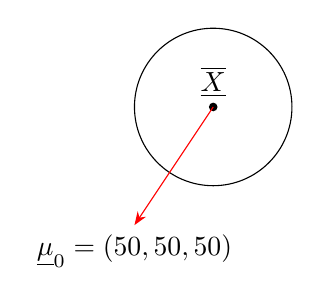
\begin{tikzpicture}[=>stealth]
\draw(0,0)circle[thick,radius=1cm];
\draw(0,0)node[shape=circle,draw,scale=0.01cm,fill=black!]{}
(0,0)node[above]{$\overline{\underline{X}}$};
\draw[-Stealth,red](0,0)--(-1,-1.5);
\draw(-1,-1.5)node[below]{$\underline{\mu}_0  = (50, 50 , 50)$};
\end{tikzpicture}
\end{figure}











So $\underline{\mu}_0=\begin{pmatrix}
50, & 50, & 50\\
\end{pmatrix}'$ is not within the confidence $(95\%)$ region.\\


\item Find the $90\%$ confidence interval for $\mu_2-\mu_3$.\\

\begin{solution}
$$F_{3,33}(0.90)=\frac{1}{2}(2.28+2.23)=2.255$$
\end{solution}

$$\mu_2 - \mu_3 = L'\underline{\mu} = \begin{pmatrix}
0, & 1, & -1\\
\end{pmatrix}
\begin{pmatrix}
\mu_1\\ \mu_2\\ \mu_3\\
\end{pmatrix}
$$

\begin{align*}
\overline{X}_2-\overline{X}_3 & \pm \sqrt{\frac{p(n-1)}{n-p}F_{p,n-p,1-\alpha}\times \frac{S_{22}-2S_{23}+S_{33}}{36}}\\\\
69.75 - 68.05 & \pm \sqrt{\frac{3\times 35}{33}\times 2.255\times \frac{422.879-2(29.929)+147.897}{36}}\\
\implies \quad  1.69 & \pm \sqrt{7.175 \times 14.192167}\\
\implies \quad  1.69 & \pm 10.0910\\
& \equiv (-8.401,11.781)\\
\end{align*}
\textbf{Question:} What implications does this interval have on $H_0:\mu_2=\mu_3$ vs $H_a:\mu_2\neq \mu_3$.
\end{enumerate}




























\pagebreak
%\chapter{\textcolor{red}{CLASSIFICATION AND DISCRIMINATION}}

\newpage

\begin{problem}
Let $\underline{X}\sim N_3(\underline{\mu},\Sigma)$ with
$$\underline{\mu} = \begin{pmatrix}1\\2\\-1\end{pmatrix},
\qquad
\Sigma = \begin{pmatrix} 4 & 1 & 0\\ 1 & 3 & 0\\ 0 & 0 & 2\end{pmatrix}.$$
Find the distribution of $X_1+X_2$, and state with reasons whether $X_3$ is
independent of $(X_1,X_2)$.
\emph{Where to start: Theorem~5.2 for the first part, Theorem~5.4 for the
second.}
\end{problem}

\begin{solution}
Take $\underline{a}=(1,1,0)'$. Then
$\underline{a}'\underline{\mu}=3$ and
$\underline{a}'\Sigma\underline{a} = 4+3+2(1) = 9$, so
$X_1+X_2\sim N(3,9)$.

$X_3$ is independent of $(X_1,X_2)$ because the corresponding off-diagonal
block of $\Sigma$ is zero and the vector is jointly normal. Without joint
normality the zero covariances would not be enough.
\end{solution}

\begin{problem}
For the same $\Sigma$, find the conditional distribution of $X_1$ given
$X_2 = x_2$, and verify that the conditional variance does not depend on
$x_2$.
\end{problem}

\begin{problem}
Show that if $\underline{X}\sim N_p(\underline{\mu},\Sigma)$ then
$\left(\underline{X}-\underline{\mu}\right)'\Sigma^{-1}
\left(\underline{X}-\underline{\mu}\right)\sim\chi^{2}_p$, and use this to
describe the shape and orientation of a $95\%$ probability region for
$\underline{X}$.
\end{problem}

\begin{problem}
An observation is within two standard deviations of the mean on each of five
variables considered separately, yet has a Mahalanobis distance placing it
beyond the $99\%$ contour. Explain how this can happen and what it indicates.
\end{problem}

\begin{solution}
Considering each variable separately ignores the correlations. If the variables
are strongly positively correlated, the joint distribution concentrates near a
line, and a point that is moderately high on some variables and moderately low
on others lies far off that line while remaining unremarkable in every margin.
The Mahalanobis distance measures departure in the metric of $\Sigma^{-1}$ and
therefore sees it.

This is the multivariate outlier that univariate screening cannot find, and it
is the practical argument for the ellipsoidal regions of this section over a
box of individual intervals.
\end{solution}

\begin{problem}
Show that $(n-1)S \sim W_p(n-1,\Sigma)$ reduces to
$(n-1)s^{2}/\sigma^{2}\sim\chi^{2}_{n-1}$ when $p=1$, and state the univariate
counterpart of the independence of $\overline{\underline{X}}$ and $S$.
\end{problem}

\begin{problem}
Using Theorem~\ref{thm:wishart}, show that $E(S)=\Sigma$ and explain why this
requires the divisor $n-1$ rather than $n$.
\end{problem}

\section{Comparison of Two Multivariate Means}

Section~5 tested a single mean vector against a fixed value. The commoner
question in practice compares two populations, and there are two distinct
designs: the observations may be paired, or the two samples may be independent.
The distinction matters as much here as it does in the univariate case, and for
the same reason.

\subsection{Paired Comparisons}

Suppose each of $n$ units is measured under two conditions, giving
$\underline{X}_{j1}$ and $\underline{X}_{j2}$ for unit $j$. The pairing must be
respected: treating $2n$ vectors as two independent samples of size $n$ throws
away the very structure the design was built to exploit.

Form the differences
$$\underline{D}_j = \underline{X}_{j1}-\underline{X}_{j2},
\qquad j = 1,\dots,n,$$
and suppose $\underline{D}_j \sim N_p\left(\underline{\delta},\Sigma_d\right)$
independently. The problem is now a one-sample problem in the differences, and
Section~5.4 applies unchanged.

\begin{thm}[Paired $T^{2}$]
\label{thm:pairedT2}
With $\overline{\underline{D}}$ and $S_d$ the sample mean and covariance of the
differences, under $H_0: \underline{\delta}=\underline{0}$
$$T^{2} = n\,\overline{\underline{D}}'\,S_d^{-1}\,\overline{\underline{D}}
\ \sim\ \frac{(n-1)p}{n-p}\,F_{p,\,n-p},$$
and $H_0$ is rejected at level $\alpha$ when $T^{2}$ exceeds
$\frac{(n-1)p}{n-p}F_{p,n-p,\alpha}$.
\end{thm}

\begin{note}
Everything about the paired analysis follows from the single act of taking
differences. The covariance between the two conditions --- which is usually
substantial, since the same unit is measured twice --- disappears into
$\Sigma_d$ and is never estimated separately. This is exactly why pairing is
worth doing: a large positive covariance makes $\Sigma_d$ small, and a small
$\Sigma_d$ makes the test sensitive.
\end{note}

\subsection{Two Independent Samples}

Now let $\underline{X}_{11},\dots,\underline{X}_{1n_1}$ be a random sample from
$N_p(\underline{\mu}_1,\Sigma)$ and
$\underline{X}_{21},\dots,\underline{X}_{2n_2}$ an independent random sample
from $N_p(\underline{\mu}_2,\Sigma)$ --- with the \emph{same} covariance matrix.

\begin{defn}[Pooled covariance matrix]
$$S_{\text{pooled}}
= \frac{(n_1-1)S_1 + (n_2-1)S_2}{n_1+n_2-2}.$$
\end{defn}

\begin{note}
This is the matrix referred to later as $\left(n_1+n_2-2\right)S$ in the MANOVA
of Section~8. Its justification is the additivity of the Wishart,
Theorem~\ref{thm:wishart}(ii): $(n_1-1)S_1$ and $(n_2-1)S_2$ are independent
$W_p(n_1-1,\Sigma)$ and $W_p(n_2-1,\Sigma)$ variates, so their sum is
$W_p(n_1+n_2-2,\Sigma)$, and dividing by its degrees of freedom gives an
unbiased estimator of the common $\Sigma$ using both samples at once.
\end{note}

\begin{thm}[Two-sample $T^{2}$]
\label{thm:twosampleT2}
Under $H_0:\underline{\mu}_1=\underline{\mu}_2$ and equal covariance matrices,
$$T^{2} = \left(\overline{\underline{X}}_1-\overline{\underline{X}}_2\right)'
\left[\left(\tfrac{1}{n_1}+\tfrac{1}{n_2}\right)S_{\text{pooled}}\right]^{-1}
\left(\overline{\underline{X}}_1-\overline{\underline{X}}_2\right)
\ \sim\ \frac{\left(n_1+n_2-2\right)p}{n_1+n_2-p-1}\,F_{p,\,n_1+n_2-p-1}.$$
\end{thm}

\begin{note}
Set $p=1$ and the statistic becomes the square of the ordinary two-sample
$t$, with $\left(\tfrac{1}{n_1}+\tfrac{1}{n_2}\right)s^{2}_{\text{pooled}}$ in
the denominator. Every multivariate statistic in this course collapses to its
univariate ancestor in this way, and checking that it does is the surest way to
remember the degrees of freedom.
\end{note}

\begin{note}[The assumption of equal covariance]
The pooling is legitimate only if $\Sigma_1=\Sigma_2$. When the covariance
matrices differ and the sample sizes are unequal, the test does not hold its
nominal level --- and the direction of the error depends on which sample is the
larger, so it cannot even be relied upon to be conservative. This is the
multivariate Behrens--Fisher problem, and it has no exact solution. Approximate
procedures replace the pooled matrix by
$\tfrac{1}{n_1}S_1+\tfrac{1}{n_2}S_2$ and adjust the degrees of freedom.

Equality can be examined by Box's $M$ test, though that test is itself sensitive
to non-normality, so a significant result may reflect the shape of the data
rather than a genuine difference in covariance. When $n_1$ and $n_2$ are close
to equal the pooled procedure is fairly robust to moderate inequality, which is
one practical argument for balanced designs.
\end{note}

\subsection{Simultaneous Confidence Statements}

A significant $T^{2}$ says the mean vectors differ but not in which variables.
Two devices answer that, and they differ in what they guarantee.

\begin{thm}[$T^{2}$ intervals]
With probability $1-\alpha$, \emph{every} linear combination
$\underline{a}'\left(\underline{\mu}_1-\underline{\mu}_2\right)$ simultaneously
satisfies
$$\underline{a}'\left(\overline{\underline{X}}_1-\overline{\underline{X}}_2\right)
\pm \sqrt{c^{2}}\,
\sqrt{\underline{a}'\left(\tfrac{1}{n_1}+\tfrac{1}{n_2}\right)S_{\text{pooled}}\,\underline{a}},$$
where $c^{2} = \frac{(n_1+n_2-2)p}{n_1+n_2-p-1}F_{p,n_1+n_2-p-1,\alpha}$.
\end{thm}

\begin{note}
The guarantee covers infinitely many linear combinations at once, including
those chosen after seeing the data, which is what makes the intervals safe for
exploration. The price is width. If only the $p$ individual components are of
interest, Bonferroni intervals using $t_{n_1+n_2-2,\,\alpha/2p}$ are shorter and
still control the overall error rate, but they cover only the $p$ comparisons
named in advance.

A common and instructive outcome is a significant $T^{2}$ with no individual
component significant. Nothing is wrong: the difference lies in a linear
combination of the variables rather than in any one of them, and finding which
combination is precisely what the discriminant function of Section~7 computes.
\end{note}

\subsection*{Practice Problems}

\begin{problem}
Explain why the differences must be taken before, not after, computing the
covariance matrix in a paired design, and what goes wrong if the $2n$
observations are treated as two independent samples.
\end{problem}

\begin{problem}
Show that Theorem~\ref{thm:twosampleT2} reduces to the square of the ordinary
two-sample $t$ statistic when $p=1$, and check that the degrees of freedom
agree.
\end{problem}

\begin{problem}
Two independent samples of sizes $n_1=25$ and $n_2=30$ are taken on $p=3$
variables. State the multiplier $c^{2}$ for simultaneous $T^{2}$ intervals at
$\alpha=0.05$, and the corresponding Bonferroni multiplier for the three
component comparisons. Which is larger, and why must it be?
\end{problem}

\begin{problem}
Using the additivity of the Wishart, prove that
$E\left(S_{\text{pooled}}\right) = \Sigma$.
\emph{Where to start: Theorem~\ref{thm:wishart} parts (i) and (ii).}
\end{problem}

\begin{problem}
A two-sample $T^{2}$ is significant at the $1\%$ level, yet no individual
variable differs significantly between the groups. Explain how this arises and
what should be reported.
\end{problem}

\begin{problem}
Discuss what happens to the level of the two-sample test when
$\Sigma_1\neq\Sigma_2$, distinguishing the cases $n_1=n_2$ and $n_1\ll n_2$.
\end{problem}


\section{Classification and Discrimination}

Discriminate analysis and classification are multivariate techniques concerned with separating distinct facts of objects (observation) and with allocating new objects (observations) to previous define groups.\\

Discriminate analysis is rather exploratory while classification require well defined rules.\\

In classification clauses of misclassifications and costs of missclassifications are sometimes taken in account when developing rules.\\
A Bayesian approach is encompassed as the way of introducing prior information.\\

Some methods assure specific distribution sources as the normal distribution.\\\\








\subsection{Fisher's Discriminant Function}
Fishers approach does not assure a particular distribution but rather assures equal covarince matrix.\\

It transforms multivariate observations $X$ to univariate observations $Y$ such that $Y's$ derivated from one population as separated as much as possible from one another population $\pi_1$ and $\pi_2$.\\

Let $\underline{Y}= L'\underline{X}$ be a linear combination of $X's$. The linear combinations transforms from the first population into the univariate data set $$Y_{11}, Y_{12}, \ldots, Y_{1n}$$ and transform $x's$ in the second population into $y_{21}, y_{22},\ldots, y_{2m}$.\\

The ideal is to look for $L$ which will separate $\overline{Y}_1$ and $\overline{Y}_2$, an illustration is given below.

% DIAGRAM 9
\begin{figure}[H]
\centering
\begin{tikzpicture}[=>stealth]
\draw[-Stealth](-3,0)--(3,0)node[right]{$x_1$};
\draw[-Stealth](0,-3)--(0,3)node[left]{$x_2$};
\draw[thick,teal,-Stealth](0,0)--(3,1)node[right]{$y_1=\underline{L}_1'\mathrm{\underline{x}}$};
\draw[thick,blue,-Stealth](0,0)--(-2,2)node[left]{$y_2 = \underline{L}_2'\mathrm{\underline{x}}$};
\draw[red,thick](-4,2)--(-2,0)--(0,-2);
\draw(-1,-1)node[left]{$\frac{1}{2}(\overline{Y}_1+\overline{Y}_2)$}
(-3.5,1.5)node[left]{pop $\pi_2$}
(-0.01,-0.5)node[left]{pop $\pi_1$};
\end{tikzpicture}
\end{figure}














In the diagram $Y_1 = L'_1\underline{X}$ leads to a population discrimination rule because it is difficult to tell the two population apart. $Y_2 = \underline{L}'_2\underline{X}$, reasonable separates the two populations.\\

The separation of the two sets univariate $Y_i'$s is assessed in terms of $\overline{Y}_1 - \overline{Y}_2$ expressed is $S.D$ units (standard deviation). \\

i.e Separation $\displaystyle{\frac{|\overline{Y}_1-\overline{Y}_2|}{S_Y}}$ , where $S_Y$  is  such that
\begin{align*}
S^2_y & = S^2\\
      & = \frac{\sum\limits^{n_1}_{j=1}(Y_{1j}-\overline{Y}_1 )^2 + \sum\limits^{n_2}_{j=1}(Y_{2j}-\overline{Y}_2)^2}{n_1+n_2-2}\\\\
      & = \frac{(n_1-1)S^2_1 + (n_2-1)S^2_1}{n_1+n_2-2}\tag{2}
\end{align*}


The task is to select $L$ which achieves maximum separation with sample means $\overline{Y}_1$ and $\overline{Y}_2$.\\


\begin{result}
The vector $\displaystyle{L' = \big(\overline{\underline{X}_1}-\overline{\underline{X}_2}\big)'S^{-1}_p}$ can be shown to be the desired choice which achieves maximum separation between $\overline{Y}_1$ and $\overline{Y}_2$.\\
\end{result}


\begin{result}
Given $\displaystyle{L' = \big(\overline{\underline{X}_1}-\overline{\underline{X}_2}\big)'S^{-1} = d'S^{-1}}$ choice of $L$ for the maximum of the separation $\displaystyle{\frac{|\overline{Y}_1-\overline{Y}_2|}{S_y}}$ is also the maximum of $D^2$ (distance)
\end{result}



\begin{align*}
D^2 & = \max \frac{\big(\overline{Y}_1-\overline{Y}_2\big)^2}{S^2_y}=\max \frac{\big(\widehat{L}'\overline{\underline{X}_1}-\widehat{L}'\overline{\underline{X}_2}\big)^2}{\widehat{L}'S_p\widehat{L}}\\\\
& = \frac{\big(\widehat{L}'\big(\overline{\underline{X}_1}-\overline{\underline{X}_2}\big)^2}{\widehat{L}'S_p\widehat{L}} = \frac{\big(\widehat{L}'d\big)^2}{\widehat{L}'S_p\widehat{L}}\\\\
& = \frac{\big(\widehat{L}'d\big)\big(\widehat{L}'d\big)}{\widehat{L}'S_p\widehat{L}}=\frac{\big(d'S_p^{-1}d\big)\big(d'S_p^{-1}d\big)}{d'S^{-1}_pS_pS^{-1}_pd}\\\\
& = \frac{\big(d'S^{-1}_pd\big)\big(d'S_p^{-1}d\big)}{d'S^{-1}_pd}\\\\
& = \big(d'S^{-1}_pd\big)\tag{3}
\end{align*}



$D^2$ is often used for discrimination \,$y_{1j}=\widehat{L}\underline{X}_{1j}$  $,  y_{2j}=\widehat{L}'\underline{X}_{2j}$


\begin{align*}
\text{Pooled}\rightarrow S^2_y & = \frac{\sum\limits^{n_1}_{j=1}\big(Y_{1j}-\overline{Y}_1\big)^2 + \sum\limits^{n_2}_{j=1}\big(Y_{2j}-\overline{Y}_2\big)^2}{n_1+n_2-2}\\\\
& = \frac{\sum\limits^{n_1}_{j=1}\Big(\widehat{L}'\underline{X}_{1j}-\widehat{L}'\overline{\underline{X}_1}\Big)^2 + \sum\limits^{n_2}_{j=1}\Big(\widehat{L}'\underline{X}_{2j}-\widehat{L}'\overline{\underline{X}_2}\Big)^2}{n_1+n_2-2}\\\\
& = \frac{\sum\limits^{n_1}_{j=1}\big(\widehat{L}'\underline{X}_{1j}-\widehat{L}'\overline{\underline{X}_1}\big)\big(\widehat{L}'\underline{X}_{1j}-\widehat{L}'\overline{\underline{X}_2}\big)' + \sum\limits^{n_2}_{j=1}\big(\widehat{L}'\underline{X}_{2j}-\widehat{L}'\overline{\underline{X}_2}\big)\big(\widehat{L}'\underline{X}_{2j}-\widehat{L}'\overline{\underline{X}_2}\big)'}{n_1 + n_2 -2}\\\\
& = \frac{\sum\limits^{n_1}_{j=1}\widehat{L}'\big(\underline{X}_{1j}-\overline{\underline{X}_1}\big)\big(\underline{X}_{1j}-\overline{\underline{X}_1}\big)'\widehat{L}+ \sum\limits^{n_2}_{j=1}\widehat{L}'\big(\underline{X}_{2j}-\overline{\underline{X}_2}\big)\big(\underline{X}_{2j}-\overline{\underline{X}_2}\big)'\widehat{L}}{n_1 + n_2 - 2}\\\\
& = \frac{\widehat{L}'\Big[\sum\limits^{n_1}\big(\underline{X}_{1j}-\overline{\underline{X}_1}\big)\big(\underline{X}_{1j}-\overline{\underline{X}_1}\big)' + \sum\limits^{n_2}\big(\underline{X}_{2j}-\overline{\underline{X}_2}\big)\big(\underline{X}_{2j}-\overline{\underline{X}_2}\big)'\Big]}{n_1 + n_2 -2}\\\\
& = \widehat{L}'\Bigg[\frac{(n_1-1)S_1 + (n_2-1)S_2}{n_1 + n_2 -2}\Bigg]\widehat{L}\\\\
& = \underbrace{\widehat{L}'}_{d'S^{-1}_p} S_p \underbrace{\widehat{L}}_{S^{-1}_pd}\\\\
\end{align*}




\begin{exa}
Budges and a test a system for obtained blood measured.
There were interested in whether the system gave results consisting with means hemoglobin (Hb) an packed call value (PCV) for men and women random blood samples from 14 females and 15 males where obtained (Hb) and (PCV) were measured using the new system. Below is partial data set from for males and females.
\end{exa}

\begin{table}[H]
\centering
\begin{tabular}{cccc}
\multicolumn{2}{c}{Females} & \multicolumn{2}{c}{Males}\\
Hb   &  PCV & Hb &  PCV\\
15.5 & 0.45 & 14.0 & 0.41\\
13.6 & 0.42 & 15.3 & 0.45\\
13.5 & 0.44 & 13.5 & 0.43\\
13.0 & 0.395& 15.8  & 0.46\\
13.3 & 0.395&15.0  & 0.43\\
\end{tabular}
\end{table}

$$\text{Calculate}\quad  D^2$$


\textbf{Data}\\
$$\text{Females}:\quad  \overline{\underline{X}_1}=
\begin{pmatrix}
13.929\\
&\\
0.41679\\
\end{pmatrix}
, 
S_1 = S_F=
\begin{pmatrix}
2.425275 & 0.040676\\
&\\
0.040676 & 0.000887\\
\end{pmatrix}
$$\\



$$\text{Males:}\quad  \overline{\underline{X}_2}=
\begin{pmatrix}
15.553\\
&\\
0.4467\\
\end{pmatrix}
, 
S_2 = S_M =
\begin{pmatrix}
1.298381 & 0.014798\\
&\\
0.014798 & 0.000320\\
\end{pmatrix}
$$\\




$$S_p = \frac{(n_F-1)S_F + (n_M-1)S_M}{n_F + n_M -2}=
\begin{pmatrix}
0.1378870 & 0.0020542\\
&\\
0.0020542 & 0.000447\\
\end{pmatrix}
$$\\




$$\implies\quad  S^{-1}_p=
\begin{pmatrix}
23.0 & -1056.5\\
&\\
-1056.5 & 70920.0\\
\end{pmatrix}
$$\\


\begin{align*}
\underline{d} & = \overline{X}_F - \overline{X}_M
 = \begin{pmatrix}
13.929 - 15.553\\
&\\
0.41679 - 0.4467\\
\end{pmatrix}\\\\
& = 
\begin{pmatrix}
-1.624\\
&\\
-0.0299\\
\end{pmatrix}\\
\end{align*}






\begin{align*}
D^2 & = \underline{d}'S^{-1}_p \underline{d}\\\\
& = \begin{pmatrix}
-1.624\\\
&\\
-0.0299\\
\end{pmatrix}'
\begin{pmatrix}
23.0 & -1056.5\\
&\\
-1056.5 & 70920.3\\
\end{pmatrix}
\begin{pmatrix}
-1.624\\\
&\\
-0.0299\\
\end{pmatrix}\\\\
& = 21.461\\\\\
\end{align*}







\pagebreak
\subsection{Fishers Classification Rule}
Fishers solution to the separation of two populations can also be used to assign a new observation $\underline{X}_0$ to one of the populations.\\

\textbf{Allocation Rule:}\\
Suppose that $\underline{x}_0$ is a new observation, Fishers allocation rule using the discrimination function is 
\begin{enumerate}
\item Allocate $\underline{x}_0$ to population 1 $(\pi_1)$, if
\begin{align*}
y_0 & = \big(\overline{\underline{X}_1}-\overline{\underline{X}_2}\big) S^{-1}_p\underline{x}_0\geq \\\\
\widehat{M} & = \frac{1}{2}\big(\overline{\underline{X}_1}-\overline{\underline{X}_2}\big)'S^{-1}_p\big(\overline{\underline{X}_1}+ \overline{\underline{X}_2}\big)\\\\
\text{or}\quad  & y_0-\widehat{M}\geq 0\\
\end{align*}



\item Allocate $\underline{x}_0$ to population 2 $(\pi_2)$ if \,
$y_0 - \widehat{M} <0\qquad \text{or}\quad  y_0<\widehat{M}$\\

\end{enumerate}





\begin{exa}
Suppose that in the previous example a new observation is obtained with Hb $= 16$ and\\ PVC $=0.46$\\
\end{exa}

How should we  classify this individual as far as gender is concerned.



\begin{align*}
y_0 & =\big(\overline{\underline{X}_F} - \overline{\underline{X}_M}\big)'S^{-1}_p\underline{x}_0\\\\
& = \begin{pmatrix}
-5.76265, & -404.761\\
\end{pmatrix}
\begin{pmatrix}
16\\
\\
0.46\\
\end{pmatrix}\\\\
& = -93.988
\end{align*}






\begin{align*}
\widehat{M} & = \frac{1}{2}\big(\overline{\underline{X}_F}-\overline{\underline{X}_M}\big)'S^{-1}_p\big(\overline{\underline{X}_F}+\overline{\underline{X}_M}\big)\\\\
& = \begin{pmatrix}
-5.76265, & -404.761\\
\end{pmatrix}
\begin{pmatrix}
14.741\\
\\
0.0432\\
\end{pmatrix}\\\\
& = -89.910\\
\end{align*}

Since $y_0 < \widehat{M}$\\
The observation $(16,0.46)$ belongs to a male participant.\\\\




\subsection{Fishers Rule Through Mahalanobie's Distance}
Let $(\pi_1)$ and $(\pi_2)$ be two populations and $\overline{\underline{X}}_1$ and $\overline{\underline{X}}_2$ be sample mean vectors respectively. Thus, let $S$ be the common sample covariance. Let $X\in \mathbb{R}^p$ assign
\begin{enumerate}
\item $\underline{X}$ to $\pi_1$ if\,
$\displaystyle{\big(\overline{X}_1 -\underline{X}\big)'S^{-1}\big(\overline{X}_1-\underline{X}\big) < \big(\overline{X}_2-\underline{X}\big)'S^{-1}\big(\overline{X}_2-\underline{X}\big)}$
$\qquad\text{or}\quad  d\big(\underline{X},\overline{X}_1\big) < d\big(\underline{X},\overline{X}_2\big)$

\item $\underline{X}$ to $\pi_2$ otherwise.\\\\
\end{enumerate}



Now,
$$\big(\overline{X}_1 - X\big)'S^{-1}\big(\overline{X}_1- X\big) < \big(\overline{X}_2-X\big)'S^{-1}\big(\overline{X}_2 - X\big)$$

$$\implies \quad  \big(\overline{X}_1 -\overline{X}_2 + \overline{X}_2 - X\big)'S^{-1}\big(\overline{X}_1 - X\big) < \big(\overline{X}_2 - \overline{X}_1 + \overline{X}_1 - X\big) S^{-1}\big(\overline{X}_2-X\big)$$

$$\big(\overline{X}_1-\overline{X}_2\big)'S^{-1}\big(\overline{X}_1-X\big) + \big(\overline{X}_2-X\big)'S^{-1}\big(\overline{X}_1-X\big) < \big(\overline{X}_2-\overline{X}_1\big)'S^{-1}\big(\overline{X}_2-X\big) + \big(\overline{X}_1-X\big)'S^{-1}\big(\overline{X}_2-X\big)$$

$$\implies \quad  \big(\overline{X}_1-\overline{X}_2\big)'S^{-1}\big(\overline{X}_1-X\big) + \big(\overline{X}_1-\overline{X}_2\big) S^{-1}\big(\overline{X}-X\big) <0$$

$$\implies \quad  \big(\overline{X}_1-\overline{X}_2\big)'S^{-1}\big(\overline{X}_1+\overline{X}_2-2X\big) < 0$$

$$\implies \quad  \big(\overline{X}_1-\overline{X}_2\big)'S^{-1}\Bigg(\frac{\overline{X}_1+\overline{X}_2}{2}-X\Bigg) < 0$$

$$\implies \quad  \big(\overline{X}_1-\overline{X}_2\big)'S^{-1}\Bigg(\frac{\overline{X}_1+\overline{X}_2}{2}\Bigg) - \big(\overline{X}_1-\overline{X}_2\big)'S^{-1}X <0$$\\\\






\subsection{More Than Two Population}
Again Fishers suggestion was to look for a linear function $a'X$ which maximized the ratio of between groups of sum of squares that is \begin{equation}\tag{5}
\underline{Y}=X\underline{a}=
\begin{pmatrix}
X_1\underline{a}\\
\vdots\\
\vdots\\
X_g\underline{a}\\
\end{pmatrix}
=\begin{pmatrix}
Y_1\\
\vdots\\
\vdots\\
Y_g\\
\end{pmatrix}
\end{equation}



where we assume there are $g$ populations, be a linear combination of the columns of $X$ , then $Y$ has total sum of squares \begin{equation}\tag{6}
\underline{Y}'H\underline{Y}=\underline{a}'X'HX\underline{a}= \underline{a}T\underline{a}
\end{equation}


which can be partitioned as a sum of the within groups (SSS) \begin{equation}\tag{7}
\sum^g_{i=1}Y_i'H_iY_i = \sum^g_{i=1}\underline{a}'X_i'H_iX_i\underline{a}_i \underline{a}'W\underline{a}
\end{equation}

plus between groups sum of squares , each $i$ for the specific group. Between groups of sum of squares can also be written as \begin{equation}\tag{8}
\sum_in_i\big(\overline{Y}_i-\overline{Y}\big)^2= \sum_i n_i\big\{\underline{a}'\big(\underline{X}_i-\overline{X}\big\} = \underline{a}'B\underline{a}
\end{equation}


where $\overline{Y}_i$ is the mean of $i^{\text{th}}$ sub vector of $Y$ and $H_i$ is the $n_i\times n_i$ centering matrix for population  $i$.\\


The Ratio of interest is given by \,$\displaystyle{\frac{\underline{a}'B\underline{a}}{\underline{a}W\underline{a}}\qquad (9)}$\\

If $\underline{a}$ is a vector which maximizes (9) the linear combination $\underline{a}'\underline{X}$ is called Fishers linear discrimination function.\\\\




\begin{thm}
The vector $\underline{a}$ in Fishers linear discrimination function is the eigen-vector of $W^{-1}B$ corresponds to the largest eigenvalue.\\\\
\end{thm}




\subsection{Sample Values}
In sample matrices for the discriminate in (9) are \begin{equation}\tag{10}
\widehat{B} = \sum^g_{i=1}\big(\underline{X}_i-\overline{\underline{X}}\big)\big(\underline{\overline{X}_i}-\overline{\underline{X}}\big)'
\end{equation}
and the sample estimate for $W$ is 
\begin{equation}\tag{11}
\widehat{W} = \sum^g_{i=1}(n_i-1)S_i = \sum^g_{i=1}\sum^{n_i}_{j=1}\big(\underline{X}_{ij}-\overline{\underline{X}_i}\big)\big(\underline{X}_{ij}-\underline{X}_i\big)'
\end{equation}

So that $\displaystyle{S_{pooled}=\frac{\widehat{W}}{n_1+n_2+\cdots+n_g-g}}\qquad (12)$\\

$\widehat{W}$ is an estimate of $\displaystyle{\Sigma}$. It can be shown that the vector $\underline{a}$ is the eigenvector of $\widehat{W}^{-1}\widehat{B}$.\\\\




\subsection{Fishers Sample Linear Discriminate}
Let $\hat{\lambda}_1,\hat{\lambda}_2,\ldots, \hat{\lambda}_s>0$ denote the $S\leq \min(g-1,p)$ non zero eigenvalues of $\widehat{W}^{-1}\widehat{B}$ and $\hat{e}_1,\hat{e}_2,\ldots, \hat{e}_s$ be the corresponding eigenvectors scaled so that $\hat{e}'$ $$\hat{e}'S_p\hat{e}=1$$

Then the vector of coefficients $\widehat{\underline{a}}= \widehat{L}$ that maximizes the ratio \begin{equation}\tag{13}
\frac{\widehat{L}'\widehat{B}\widehat{L}}{\widehat{L}'\widehat{W}\widehat{L}}=\frac{\widehat{L}'\Bigg(\sum\limits^g_{i=1}\big(\overline{X}_i-\overline{X}\big)\big(\overline{X}_i-\overline{X}\big)'\Bigg)\widehat{L}}{\widehat{L}'\Bigg(\sum\limits^g_{i=1}\sum\limits^{n_i}_{j=1}\big(X_{ij}-\overline{X}_i\big)\big(X_{ij}-\overline{X}_i\big)'\Bigg)\widehat{L}}
\end{equation}

is given by $\widehat{L}_1=\widehat{e}_1$. The linear combination $\widehat{L}_1X$ is called the sample first discriminate. The choice $\widehat{L}_2 =\widehat{e}_2$ produces the sample second discriminate. Continuing we have that $$\widehat{L}'_kX =\widehat{e}'_kX$$ is the sample $k^{\text{th}}$ discriminate $k\leq S$.\\\\


Sketch of proof of the Theorem on $\displaystyle{\frac{\underline{a}'B\underline{a}}{\underline{a}'W\underline{a}}}$.\\

Let $\displaystyle{f=\frac{\underline{a}'B\underline{a}}{\underline{a}'W\underline{a}}\in \mathbb{R}}$\\

$\implies \quad  f\underline{a}'W\underline{a} = \underline{a}'B\underline{a}$ post multiplying by $\underline{a}$\\

$\implies \quad  \underline{a}\cdot \underline{a}' W \underline{a} = \underline{a}\cdot \underline{a}'B \underline{a}$\\

Assume $\underline{a}\, \underline{a}' >0$, pre-multiplying

$$f(\underline{a}\,\underline{a}')^{_1} \underline{a}\, \underline{a}' W \underline{a} = (\underline{a}\,\underline{a}')^{-1}\underline{a}\, \underline{a}'B\underline{a}$$

$$\implies \quad  fW\underline{a} = B\underline{a}$$

$W>0$ then $fW^{-1} W \underline{a} = W^{-1}B\underline{a}\quad \implies \quad  f\underline{a} = W^{-1}B\underline{a}$.\\\\



\subsection{Fishers Classification Procedure Based of On Sample Discriminate}
Allocate $X$ to $\pi_k$ if
\begin{align*}
\sum^r_{j=1}\big(\widehat{Y}_j-\overline{Y}_{kj}\big)^2 & = \sum^r_{j=1}\big[\widehat{L}'_j\big(X-\overline{X}\big)\big]^2\\
& = \sum^r_{j=1}\big[\widehat{e}'_j\big(X-\overline{X}_j\big)\big]^2\qquad\text{for all}\quad  j\neq k\\
\end{align*}



























\pagebreak
%\chapter{\textcolor{red}{ANALYSIS OF VARIANCE}}

\subsection{Practice Problems}

\begin{problem}
Fisher's linear discriminant maximises the ratio
$$\frac{\left[\underline{a}'\left(\overline{\underline{x}}_1-\overline{\underline{x}}_2\right)\right]^{2}}
{\underline{a}'S_{\text{pooled}}\,\underline{a}}.$$
Show that the maximum is attained at
$\underline{a}\propto S_{\text{pooled}}^{-1}
\left(\overline{\underline{x}}_1-\overline{\underline{x}}_2\right)$.
\emph{Where to start: the same weighted-average argument as
Theorem~4.4, applied after the substitution
$\underline{b} = S_{\text{pooled}}^{1/2}\underline{a}$.}
\end{problem}

\begin{problem}
Show that the maximised value of that ratio is the squared Mahalanobis distance
between the two sample means, and explain why this makes it a natural measure of
separation.
\end{problem}

\begin{problem}
Explain why a discriminant analysis and a principal component analysis of the
same data can point in quite different directions, and construct a
two-dimensional example in which the first principal component is useless for
separating two known groups.
\emph{Where to start: let the groups differ along the direction of least
variation.}
\end{problem}

\begin{solution}
Take two groups whose members are spread widely along $x_1$ and only slightly
along $x_2$, with the two group means differing only in $x_2$. The first
principal component is then almost exactly $x_1$, along which the groups
completely overlap; the discriminant is almost exactly $x_2$, along which they
separate cleanly.

The moral is the one stated in Section~4.5: principal components maximise
variance, and variance is not separation. Using the leading components as a
preliminary to classification can discard precisely the direction that
classifies.
\end{solution}

\begin{problem}
State Fisher's classification rule for two populations in terms of the
discriminant score, and show that with equal prior probabilities and equal
misclassification costs it assigns $\underline{x}$ to the population whose mean
is nearer in Mahalanobis distance.
\end{problem}

\begin{problem}
The apparent error rate is computed by classifying the same observations used to
fit the rule. Explain why it is optimistically biased, and describe two ways of
obtaining a more honest estimate.
\end{problem}

\begin{solution}
The rule is chosen to separate the observations in hand, so it is fitted partly
to their noise as well as to the structure; scored on those same observations it
is being credited for recognising cases it has already seen. The bias grows with
the number of variables relative to the sample size.

Two remedies. A holdout sample fits the rule on part of the data and scores it
on the rest, which is unbiased but wastes observations. Cross-validation, in the
leave-one-out form, classifies each observation using a rule fitted without it,
which uses every observation and is nearly unbiased at the cost of $n$ fits.
This is the same concern, and the same remedy, as the honest accuracy discussed
for any fitted classifier.
\end{solution}

\begin{problem}
For more than two populations, explain how the discriminant directions arise as
eigenvectors of $W^{-1}B$, and state how many non-zero eigenvalues there can be
when there are $g$ groups and $p$ variables.
\end{problem}

\section{Multivariate Analysis of Variance (MANOVA)}
Suppose in the discrimination problem encountered earlier we wished to test the hypothesis equality of means. Specifically we wish to test $H_0:\underline{\mu}_1 = \underline{\mu}_2 = \cdots= \underline{\mu}_n$ the way of the univariate case of testing $H_0: \mu_1 = \mu_2 = \cdots= \mu_n$.\\

How do we proceed?\\

Using the univariate analog we set up a multivariate model \begin{equation}\tag{1}
\underline{X}_{ij}= \underline{\mu} + \tau _i + \underline{e}_{ij},  j=1,2,\ldots,n_i\qquad i=1,2,\ldots,g
\end{equation}
where $e_{ij}$ are independent $N_p\big(\underline{0},\Sigma\big)$ (multivariate normal) variables (vectors) we have the parameter vector $\underline{\mu}$ is an overall mean and $\tau_i$ represents the $i^{\text{th}}$ treatment effect with $\sum\limits^g_{i=1}n_i\tau_i= \underline{0}$.\\


The model in (1) may also be represented as \begin{equation}\tag{2}
\underline{X}_{ij} =\underline{\mu}_i + \underline{e}_{ij},  e_{ij}\thicksim^{iid}N_p\big(\underline{0},\Sigma\big)
\end{equation}
 where $\mu_i = \underline{\mu} + \underline{\tau}_i$\\
 
 In model (1) we note the following 
\begin{enumerate}
\item[$-$] each component of the observation vector 
\,$ \underline{X}_{ij}=
\begin{pmatrix}
X_{ij1} & X_{ij2} & \cdots& X_{ijp}\\
\end{pmatrix}'\,$ satisfies the univariate model $$X_{ij} = \mu + \tau_i + e_{ij} \quad  e_{ij} \thicksim^{iid} N(0,\sigma^2)$$
\item[$-$] the errors of the components of $\underline{X}_{ij}$ are correlated but $\Sigma$ covariance is the same for all populations.\\
\end{enumerate}



\subsection{Incorporating Data}
 A vector of observations may be decomposed as follows:

% DIAGRAM 10
\begin{figure}[H]
\centering
\begin{tikzpicture}[=>stealth]
\draw(-3,0)--(3,0);
\draw(-2,0)node[]{$|$}
(0,0)node[]{$|$}
(2,0)node[]{$|$};
\draw(-2,-0.1)node[below]{$X_{ij}$}
(0,-0.1)node[below]{$\overline{X}_j$}
(2,-0.1)node[below]{$\overline{X}$};
\draw[|-|](-2,-1)--(2,-1);
\end{tikzpicture}
\end{figure}







\begin{equation}\tag{4}
X_{ij}-\overline{X} = \overline{X}_i-\overline{X} + \big(X_{ij} - \overline{X}_i\big)
\end{equation}
where
\begin{enumerate}
\item[] $\underline{X}_{ij}=$ observation
\item[] $\overline{\underline{X}}=$ overall sample mean, $\underline{\hat{\mu}}$
\item[] $\overline{X}_i- \overline{X} = $ Estimate of treatment effect $\tau_i$
\item[] $X_{ij} -\overline{X}_i =$ Residual estimate of error, $\hat{e}_{ij}$\\
\end{enumerate}


The decomposition (4) leads to the univariate analog of univariates sum of squares break up specifically (1) the left hand side becomes $$\sum^g_{i=1}\sum^{n_i}_{j=1}\big(\underline{X}_{ij}-\underline{\overline{X}}\big)\big(\underline{X}_{ij}-\overline{\underline{X}}\big)'$$

as the total corrected sum of squares and cross products\\

\begin{equation}\tag{5}
2.1\qquad  \sum^g_{i}n_i\big(\overline{\underline{X}}_i-\overline{\underline{X}}\big)\big(\overline{\underline{X}}_i-\overline{\underline{X}}\big)'
\end{equation}
As the Between treatments sum of  squares and cross products 
 
\begin{equation}\tag{6}
2.2\qquad  \sum^g_{i=1}\sum^{n_i}_{j=1}\big(\underline{X}_{ij}-\overline{\underline{X}}_i\big)\big(\underline{X}_{ij}-\overline{\underline{X}}_i\big)'
\end{equation}

As the residual within sum of squares and cross products.\\

2.2 can also be expressed as follows
\begin{align*}
\textbf{W} & = \sum^g_{i=1}\sum^{n_i}_{j=1}\big(\underline{X}_{ij}-\overline{\underline{X}}_i\big)\big(\underline{X}_{ij}-\overline{\underline{X}}_i\big)'\\
& = \sum^g_{i=1}(n_i-1)S_i\\
& = (n_1-1)S_1 + (n_2-1)S_2 + \cdots+ (n_g-1)S_g\tag{7}
\end{align*}

The matrix generalization, where $S_i$ is the sample covariance matrix for the $i^{\text{th}}$ sample group.\\

$(n_1+n_2-2)S$ pooled matrix encountered in the two sample situation.\\\\

To test the hypothesis of no treatment effect.
$$H_0: \underline{\tau_1} = \underline{\tau_2} = \cdots= \underline{\tau_g}=\underline{0} \qquad \text{or}\quad  H_0: \underline{\mu_1} = \underline{\mu_2}=\cdots= \underline{\mu_g}$$

\begin{align*}
\underline{\mu}_1 & = \underline{\mu} + \underline{\tau}_1\\
\underline{\mu}_2 & = \underline{\mu} + \underline{\tau}_2\\
\vdots & \\
\underline{\mu}_g & = \underline{\mu} + \underline{\tau}_g\\\\
\sum \underline{\mu}_i & = g\underline{\mu} + \sum \underline{\tau}_i
\end{align*}

We utilize the relative sizes of the residual and total (corrected sum of  squares and cross products matrix terms). The results are often summarized in the table known as the MANOVA


\begin{table}[H]
\centering
\begin{tabular}{|c|c|c|}
\hline
Source of & Matrix of $SS$ & Degrees of\\
Variation & and Cross Products & Freedom $(df)$\\
\hline
&&\\
Treatment & $\textbf{B}=\displaystyle{\sum^g_{i=1}n_i\big(\overline{\underline{X}}_i-\overline{\underline{X}}\big)\big(\overline{\underline{X}}_i-\overline{\underline{X}}\big)'}$ & $g-1$\\
&&\\
Residual (Error) & $\textbf{W}=\displaystyle{\sum^g_{i=1}\sum^{n_i}_{j=1}\big(\underline{X}_{ij}-\overline{\underline{X}_i}\big)\big(\underline{X}_{ij}-\overline{\underline{X}_i}\big)'}$ & $\displaystyle{\sum^g_{i=1}n_i-g}$\\
&&\\
\hline
Total (corrected) & $\textbf{B}+ \textbf{W}=\displaystyle{\sum^g_{i=1}\sum^{n_i}_{j=1}\big(\underline{X}_{ij}-\overline{\underline{X}}\big)\big(\underline{X}_{ij}-\overline{\underline{X}}\big)'}$ & $\displaystyle{\sum^g_{i=1}n_i-1}$\\
For the Mean &&\\
\hline
\end{tabular}
\caption{}
\end{table}


$$X_{ij} = \mu + \tau_i + e_{ij} \thicksim N_p\big(\underline{0},\Sigma\big)\qquad \text{estimates}\quad  X_{ij}=\underline{\overline{X}}+\overline{\underline{X_i}}\cdot \overline{\underline{X}} + X_{ij}-\overline{\underline{X}_i}$$

The degrees of freedom correspond to the univariate geometric and also to multivariate distribution theory of the Wishart densities.\\

The test of $H_0: \underline{\tau}_1 = \underline{\tau}_2 = \cdots= \underline{\tau}_g = \underline{0}$ utilize the Wilk's Lambda
\begin{align*}
\Delta_W & = \frac{\Big|\textbf{W}\Big|}{\Big|\textbf{B}+\textbf{W}\Big|}\\\\
& = \frac{\Bigg|\displaystyle{\sum^g_{i=1}\sum^{n_i}_{j=1}\big(\underline{X}_{ij}-\overline{\underline{X}_i}\big)\big(\underline{X}_{ij}-\overline{\underline{X}_i}\big)'}\Bigg|}{\Bigg|\displaystyle{\sum^g_{i=1}\sum^{n_i}_{j=1}\big(\underline{X}_{ij}-\overline{\underline{X}}\big)\big(\underline{X}_{ij}-\overline{\underline{X}}\big)'}\Bigg|}\tag{9}
\end{align*}


% DIAGRAM 11
\begin{figure}[H]
\centering
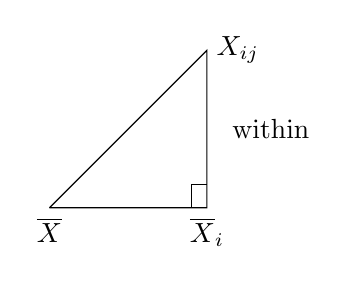
\begin{tikzpicture}[=>stealth]
\draw(-4,0)--(-2,0)--(-2,2)--(-4,0);
\draw(-4,0)node[below]{$\overline{X}$}
(-2,0)node[below]{$\overline{X}_i$}
(-2,2)node[right]{$X_{ij}$};
\draw(-2.2,0)--(-2.2,0.3)--(-2,0.3);
\draw(-1.8,1)node[right]{within};
\end{tikzpicture}
\qquad 
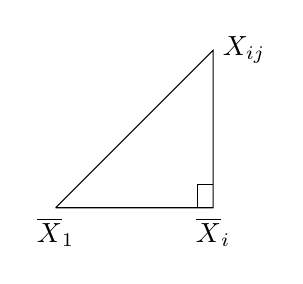
\begin{tikzpicture}[=>stealth]
\draw(2,0)--(4,0)--(4,2)--(2,0);
\draw(2,0)node[below]{$\overline{X}_1$}
(4,0)node[below]{$\overline{X}_i$}
(4,2)node[right]{$X_{ij}$};
\draw(3.8,0)--(3.8,0.3)--(4,0.3);
\end{tikzpicture}
\end{figure}














There are various cases of which $\Delta$ leads to exact distributions.
\begin{table}[H]
\centering
\caption{ DISTRIBUTION OF WILKS' LAMBDA}
\begin{tabular}{ccc}
\hline
No. of & No. of & \\
variables & groups & Sampling distributions for multivariate normal data\\
\hline
$P=1$ & $g\geq 2$ & $\Bigg(\frac{\sum n_i-g}{g-1}\Bigg)\Bigg(\frac{1-\Delta}{\Delta}\Bigg)\thicksim F_{g-1,\sum n_i-g}$\\
&&\\
$p=2$ & $g\geq 2$ & $\Bigg(\frac{\sum n_i-g-1}{g-1}\Bigg)\Bigg(\frac{1-\sqrt{\Delta}}{\sqrt{\Delta}}\Bigg)\thicksim F_{2(g-1),2(\sum n_i-g-1)}$\\
&&\\
$p\geq 1$ & $g=2$ & $\Bigg(\frac{\sum n_i-p-1}{p}\Bigg)\Bigg(\frac{1-\Delta}{\Delta}\Bigg)\thicksim F_{p,\sum n_i-p-1}$\\
&&\\
$p\geq 1$ & $g=2$ & $\Bigg(\frac{\sum n_i - p -2}{p}\Bigg)\Bigg(\frac{1-\sqrt{\Delta}}{\sqrt{\Delta}}\Bigg)\thicksim F_{2p,2(\sum n_i-p-2)}$\\
&&\\
\hline
\end{tabular}
\end{table}


\begin{align*}
& Pr\big(\ln \Delta^* < \ln \Delta^*_c = \Delta'_c\big)\\
& Pr\Big(-\big(n-1-\frac{p+g}{2}\big)\ln \Delta^* < \Delta'_c\Big)\\
& Pr\Big(\chi^2_{p(g-1)}\leq \Delta_c\Big)= \alpha\\
\end{align*}






\begin{exa}
Suppose that an experiment was performed in which 4 groups of students were sent to interview holds on certain issues. For correctness, suppose that there were $n=3$ students per group and 2 questions were asked on each house hold the expenses on the house hold in previous months in each month recorded separate. The data imaginary are recorded in the following table in 100's of kwacha.\\
\end{exa}


\begin{table}[H]
\centering
\begin{tabular}{cccc}
\hline
&\multicolumn{3}{c}{measurements (100's of Kwacha)}\\\\
Group & Student & Month 1 & Month 2\\
\hline
 & 1 & 4 & 6\\
1& 2 & 2 & 5\\
 & 3 & 3 & 4\\
\hline 
 & 1 & 4 & 5\\
2& 2 & 5 & 4\\
 & 3 & 6 & 6\\
\hline
 & 1 & 6 & 6\\
3& 2 & 7 & 8\\
 & 3 & 8 & 7\\
\hline 
 & 1 & 7 & 6\\
4& 2 & 9 & 8\\
 & 3 & 8 & 7\\
\hline
\end{tabular}
\end{table}


Test for the difference in mean vector in the four groups.$$H_0: \underline{\mu}_1 = \underline{\mu}_2=\underline{\mu}_3=\underline{\mu}_4$$
\begin{solution}
$$X_{ij} \thicksim N_2\big(\underline{\mu}_i,\Sigma\big),  i=1,2,3,4$$
\end{solution}

$$\overline{X}=\begin{pmatrix}
\overline{X}_1\\ \overline{X}_2\\
\end{pmatrix}=
\begin{pmatrix}
\sum X_{1j}/12\\ \sum X_{2j}/12\\
\end{pmatrix}=
\begin{pmatrix}
5.75\\ 6\\
\end{pmatrix}
$$\\

$$n_1=3;\quad  \overline{X}_1=\begin{pmatrix}
(4+2+3)/3\\ (6+5+4)/3\\
\end{pmatrix}=
\begin{pmatrix}
3\\ 5\\
\end{pmatrix}
$$\\

$$n_2=3;\quad  \overline{X}_2=
\begin{pmatrix}
5\\ 5\\
\end{pmatrix}
$$\\


$$\overline{X}_3=
\begin{pmatrix}
7\\7\\
\end{pmatrix}
\qquad 
\overline{X}_4=
\begin{pmatrix}
8\\ 7\\
\end{pmatrix}
$$\\


\begin{align*}
\textbf{B} & = \sum^g_in_i\big(\overline{\underline{X}_i}-\overline{\underline{X}}\big)\big(\overline{\underline{X}_i}-\overline{\underline{X}}\big)'\\
& = \sum^4_1 3\big(\overline{\underline{X}_i}-\overline{\underline{X}}\big)\big(\overline{\underline{X}_i}-\overline{\underline{X}}\big)'\\
& = 3\begin{pmatrix}
-2.75\\ -1\\
\end{pmatrix}
\begin{pmatrix}
-2.75 & -1\\
\end{pmatrix} + 3\begin{pmatrix}
-0.75\\ 1\\
\end{pmatrix}
\begin{pmatrix}
-0.75 & 1\\
\end{pmatrix}\\
&
 + 3 \begin{pmatrix}
1.25\\1\\
\end{pmatrix}
\begin{pmatrix}
1.25 & 1\\
\end{pmatrix}
+ 3\begin{pmatrix}
2.25\\ 1\\
\end{pmatrix}
\begin{pmatrix}
2.25 & 1\\
\end{pmatrix}\\\\
\implies \quad  \textbf{B}& = \begin{pmatrix}
44.25 & 21\\
21 & 12.00\\
\end{pmatrix}\\\\
\end{align*}




$$ \textbf{W}= \sum^4_{i=1}\sum^3_{j=1}\big(\underline{X}_{ij}-\overline{X}_i\big)\big(\underline{X}_{ij}-\overline{X}_i\big)'$$

\begin{align*}
G_1: & \begin{pmatrix}
1\\ 1\\
\end{pmatrix}
\begin{pmatrix}
1, & 1\\
\end{pmatrix} + \begin{pmatrix}
-1\\ 0\\
\end{pmatrix}
\begin{pmatrix}
-1, & 0\\
\end{pmatrix} + \begin{pmatrix}
0\\ -1\\
\end{pmatrix}
\begin{pmatrix}
0, & -1\\
\end{pmatrix}\\\\
& = 
\begin{pmatrix}
1 & 1\\
1 & 1\\
\end{pmatrix} + \begin{pmatrix}
1 & 0\\
0 & 0\\
\end{pmatrix} + \begin{pmatrix}
0 & 0\\
0 & 1\\
\end{pmatrix}\\\\
& = \begin{pmatrix}
2 & 1\\
1 & 2\\
\end{pmatrix}\\
\end{align*}



\begin{align*}
G_2: & \begin{pmatrix}
-1\\0\\
\end{pmatrix}
\begin{pmatrix}
-1, & 0\\
\end{pmatrix} + \begin{pmatrix}
0\\ -1\\
\end{pmatrix}
\begin{pmatrix}
0, & -1\\
\end{pmatrix} + \begin{pmatrix}
1\\1\\
\end{pmatrix}
\begin{pmatrix}
1, & 1\\
\end{pmatrix}\\\\
& =\begin{pmatrix}
1 & 0\\
0 & 0\\
\end{pmatrix} + \begin{pmatrix}
0 & 0\\
0 & 1\\
\end{pmatrix} + \begin{pmatrix}
1 & 1\\
1 & 1\\
\end{pmatrix}\\\\
& = \begin{pmatrix}
2 & 1\\
1 & 2\\
\end{pmatrix}\\
\end{align*}





\begin{align*}
G_3: & \begin{pmatrix}
-1\\-1\\
\end{pmatrix}
\begin{pmatrix}
-1, & -1\\
\end{pmatrix} + \begin{pmatrix}
0\\ 1\\
\end{pmatrix}
\begin{pmatrix}
0, & 1\\
\end{pmatrix} + \begin{pmatrix}
1\\0\\
\end{pmatrix}
\begin{pmatrix}
1, & 0\\
\end{pmatrix}\\\\
& = \begin{pmatrix}
1 & 1\\
1 & 1\\
\end{pmatrix} + \begin{pmatrix}
0 & 0\\
0 & 1\\
\end{pmatrix} + \begin{pmatrix}
1 & 0\\
0 & 0\\
\end{pmatrix}\\
& = \begin{pmatrix}
2 & 1\\
1 & 2\\
\end{pmatrix}\\
\end{align*}



\begin{align*}
G_4: & \begin{pmatrix}
-1\\ -1\\
\end{pmatrix}
\begin{pmatrix}
-1, & -1\\
\end{pmatrix} + \begin{pmatrix}
1\\ 1\\
\end{pmatrix}
\begin{pmatrix}
1, & 1\\
\end{pmatrix} + \begin{pmatrix}
0 \\ 0\\
\end{pmatrix}
\begin{pmatrix}
0, & 0\\
\end{pmatrix}\\\\
& = \begin{pmatrix}
1 & 1\\
1 & 1\\
\end{pmatrix} + \begin{pmatrix}
1 & 1\\
1 & 1\\
\end{pmatrix} + \begin{pmatrix}
0 & 0\\
0 & 0\
\end{pmatrix}\\\\
& = \begin{pmatrix}
2 & 2\\
2 & 2\\
\end{pmatrix}\\
\end{align*}







\begin{align*}
\implies \quad  \textbf{W} & = G_1 + G_2 + G_3 + G_4\\
& = \begin{pmatrix}
2 & 1\\
1 & 2\\
\end{pmatrix}
+ \begin{pmatrix}
2 & 1\\
1 & 2\\
\end{pmatrix} + \begin{pmatrix}
2 & 1\\
1 & 2\\
\end{pmatrix} +\begin{pmatrix}
2 & 2\\
2 & 2\\
\end{pmatrix}\\\\
\textbf{W} & = \begin{pmatrix}
8 & 5\\
5 & 8\\
\end{pmatrix}\\\\
\end{align*}











Wilks' Lambda $\Delta$ statistic is 
\begin{align*}
\Delta & = \frac{\Big|\textbf{W}\Big|}{\Big|\textbf{B}+\textbf{W}\Big|}
 = \frac{
\begin{vmatrix}
8 & 5\\
5 & 8\\
\end{vmatrix}
}{
\begin{vmatrix}
52.25 & 26\\
26 & 20\\
\end{vmatrix}
}\\\\
& = \frac{64-25}{1045-676}=\frac{39}{369}\\\\
& = 0.106\\
\end{align*}

$$p=2,  g\geq 2\qquad  \Bigg(\frac{\sum n_i-g-1}{g-1}\Bigg)\Bigg(\frac{1-\sqrt{\Delta}}{\sqrt{\Delta}}\Bigg)\thicksim F_{2,(g-1)}$$

$$\implies\quad  g=4,  2(g-1)=2(3)=6$$

$$2\big(\sum n_i -g-1\big) = 2 (12-4-1) =14$$

$$F_{6,14,0.95}=2.85$$\\

$$F_{obse} = \Bigg(\frac{12-5}{3}\Bigg)\Bigg(\frac{1-\sqrt{0.10569}}{\sqrt{0.10569}}\Bigg)=4.8439$$

Since $F_{obse} = 4.84>2.85$ we reject $H_0$ and conclude the average means of expenditure are different for the four groups.\\






















\pagebreak
%\chapter{\textcolor{red}{MULTIPLE REGRESSION}}
\subsection{Two-Way MANOVA}

The model above has a single factor. When units are classified by two factors
simultaneously the univariate two-way analysis of variance generalises in the
same way, and the additional term it brings --- interaction --- is usually the
one of real interest.

For factors $A$ at $g$ levels and $B$ at $b$ levels, with $n$ replicates in each
cell, the model is
$$\underline{X}_{\ell k r} = \underline{\mu} + \underline{\tau}_{\ell}
+ \underline{\beta}_{k} + \underline{\gamma}_{\ell k} + \underline{e}_{\ell k r},$$
where $\underline{\tau}_\ell$ is the effect of level $\ell$ of $A$,
$\underline{\beta}_k$ that of level $k$ of $B$, $\underline{\gamma}_{\ell k}$
their interaction, and the errors are independent
$N_p\left(\underline{0},\Sigma\right)$. The effects are constrained to sum to
zero over each index, as in the univariate case.

The total sum of squares and cross-products decomposes exactly as the univariate
total sum of squares does, but into matrices rather than scalars:
$$SSP_{\text{tot}} = SSP_{A} + SSP_{B} + SSP_{AB} + SSP_{\text{res}} .$$

\begin{table}[H]
\centering
\small
\begin{tabular}{|l|c|c|}
\hline
\textbf{Source} & \textbf{SSP matrix} & \textbf{d.f.}\\
\hline
Factor $A$ & $SSP_A$ & $g-1$\\
Factor $B$ & $SSP_B$ & $b-1$\\
Interaction $AB$ & $SSP_{AB}$ & $(g-1)(b-1)$\\
Residual & $SSP_{\text{res}}$ & $gb(n-1)$\\
\hline
Total & $SSP_{\text{tot}}$ & $gbn-1$\\
\hline
\end{tabular}
\caption{The two-way multivariate analysis of variance table. Each entry is a
$p\times p$ matrix; setting $p=1$ recovers the familiar univariate table.}
\label{tab:twowaymanova}
\end{table}

Each effect is tested by its own Wilks' lambda, formed against the residual
matrix:
$$\Lambda_A = \frac{\left|SSP_{\text{res}}\right|}
{\left|SSP_A + SSP_{\text{res}}\right|},$$
and similarly for $B$ and for the interaction, each referred to its own degrees
of freedom by the approximations of Section~5.5.

\begin{note}
Test the interaction first. If $\underline{\gamma}_{\ell k}$ is non-zero the
effect of factor $A$ depends on the level of $B$, and a statement about $A$
averaged over $B$ describes a situation that does not occur at any level of
$B$ --- the main-effect tests are then answering a question nobody asked. Only
when the interaction is absent do the main effects have their simple reading.
This is the same discipline as in univariate two-way analysis of variance, and
it is more easily forgotten here because the output is bulkier.
\end{note}

\begin{note}
Each cell must contain $n\geq2$ replicates for $SSP_{\text{res}}$ to have any
degrees of freedom, and $gb(n-1)\geq p$ for it to be invertible ---
Theorem~\ref{thm:wishart}(iv) again. With one observation per cell the interaction is
inseparable from the error and cannot be tested at all.
\end{note}



\subsection{Practice Problems}

\begin{problem}
State the one-way MANOVA model, its assumptions, and the decomposition
$SSP_{\text{tot}} = SSP_{\text{tr}} + SSP_{\text{res}}$. What is the univariate
statement of which this is the generalisation?
\end{problem}

\begin{problem}
Wilks' lambda is
$\Lambda = \left|SSP_{\text{res}}\right|/\left|SSP_{\text{res}}+SSP_{\text{tr}}\right|$.
Explain why small values of $\Lambda$ are evidence against equality of the mean
vectors, and why the statistic uses determinants rather than traces.
\emph{Where to start: the determinant is the generalised variance of
Section~3.4; compare what a determinant and a trace each measure.}
\end{problem}

\begin{solution}
$SSP_{\text{res}}$ measures scatter within groups and the denominator measures
total scatter. If the group means coincide, treatment contributes nothing and
the two are close, so $\Lambda$ is near one; the further apart the means, the
larger the denominator and the smaller $\Lambda$.

Determinants are used because the generalised variance measures the volume the
scatter occupies, and volume responds to separation in \emph{any} direction,
including a direction that is a combination of the variables. A trace would add
the marginal variances and could miss a separation that shows in no single
variable - the same phenomenon as the significant $T^{2}$ with no significant
component in Section~6.3.
\end{solution}

\begin{problem}
For $g=2$ groups, show that Wilks' lambda is a monotone function of the
two-sample $T^{2}$ of Theorem~\ref{thm:twosampleT2}, so that the two tests
agree.
\end{problem}

\begin{problem}
In a two-way MANOVA the interaction is significant. Explain why the main effect
tests should not then be interpreted in the usual way, and what should be
reported instead.
\end{problem}

\begin{problem}
An experiment has $g=3$ treatments, $b=2$ blocks, $p=4$ responses and $n=2$
replicates per cell. Write out the degrees of freedom for each line of the
analysis, and check that the residual matrix is invertible.
\emph{Where to start: the residual has $gb(n-1)$ degrees of freedom, and needs
at least $p$ of them.}
\end{problem}

\begin{problem}
Explain why a MANOVA on $p$ responses is preferable to $p$ separate univariate
analyses of variance, giving two distinct reasons.
\end{problem}

\section{Multivariate Multiple Regression}
In this section we consider the problem of modeling the relationship between $m$ responses $(Y_1,Y_2,\ldots,Y_m)$ and a single set of predictor variables $(Z_1,Z_2,\ldots,Z_r)$ each response is assumed to follow its own regression model so that 

\begin{align*}
Y_1 & = \beta_{01} + \beta_{11}Z_1 + \cdots+ \beta_{n1}Z_n + \varepsilon_1\\
Y_2 & = \beta_{02} + \beta_{12}Z_2 + \cdots+ \beta_{n2}Z_n + \varepsilon_2\\
\vdots &\\
Y_m & = \beta_{0m} + \beta_{1m}Z_{m} + \cdots+ \beta_{nm}Z_{n} + \varepsilon_{m}\\
\end{align*}
Let the all the equation be (1)\\

The error term $\underline{\varepsilon}=
\begin{bmatrix}
\varepsilon_1 & \varepsilon_2 & \cdots& \varepsilon_n\\
\end{bmatrix}'
$ has $E(\underline{\varepsilon})=\underline{0}$ and $var(\underline{\varepsilon})=\Sigma$.\\

\subsection{The Model and Its Notation}
To establish notation conforming to the classical linear model.\\
Let $\begin{bmatrix}
Z_{j0}, & Z_{j1}, \ldots& Z_{jn}\\
\end{bmatrix}
$ denote values for the predictor variables for the $j^{\text{th}}$ trial.\\
Let $\underline{Y}_j=
\begin{pmatrix}
Y_{j1} &  Y_{j2} & \cdots& Y_{jn}\\
\end{pmatrix}'$ be the responses and let $\underline{\varepsilon}_j = 
\begin{pmatrix}
\varepsilon_{j1} & \varepsilon_{j2} & \cdots& \varepsilon_{jn}\\
\end{pmatrix}'$ be the errors.\\
In matrix notation the design matrix
$$ Z_{n \times (r+1)} = 
\begin{pmatrix}
Z_{10} & Z_{11} & \cdots& Z_{1r}\\
Z_{20} & Z_{21} & \cdots& Z_{2r}\\
\vdots & \vdots &                    & \vdots\\
Z_{n0} & Z_{n1} & \cdots& Z_{nr}\\
\end{pmatrix}
$$


this is same as that for a single response regression model. The other matrix multivariate counter parts

$$Y_{n\times m} = 
\begin{pmatrix}
Y_{11} & Y_{12} & \cdots& Y_{1m}\\
Y_{21} & Y_{22} & \cdots& Y_{2m}\\
\vdots & \vdots &                    & \vdots\\
Y_{n1} & Y_{n2} & \cdots& Y_{nm}\\
\end{pmatrix}
=
\begin{bmatrix}
\underline{Y}_{(1)} & \vdots & \underline{Y}_{(2)} & \vdots & \cdots& \vdots & \underline{Y}_{(m)}\\
\end{bmatrix}
$$\\


$$B_{(r+1)\times m} = 
\begin{pmatrix}
\beta_{01} & \beta_{02} & \cdots& \beta_{0m}\\
\beta_{11} & \beta_{12} & \cdots& \beta_{1m}\\
\vdots     & \vdots     &                    & \vdots\\
\beta_{r1} & \beta_{r2} & \cdots& \beta_{rm}\\
\end{pmatrix}
=
\begin{bmatrix}
\underline{B}_{(1)} & \vdots & \underline{B}_{(2)} & \vdots & \cdots& \vdots & \underline{B}_{(m)}\\
\end{bmatrix}
$$

and 

$$ \varepsilon_{n\times m} = 
\begin{pmatrix}
\varepsilon_{11} & \varepsilon_{12} & \cdots& \varepsilon_{1m}\\
\varepsilon_{21} & \varepsilon_{22} & \cdots& \varepsilon_{2m}\\
\vdots           &  \vdots                &               &\vdots \\
\varepsilon_{n1} & \varepsilon_{n2} &\cdots& \varepsilon_{nm}\\
\end{pmatrix}
=
\begin{bmatrix}
\underline{\varepsilon}_{(1)} & \vdots & \underline{\varepsilon}_{(2)} & \vdots & \cdots& \vdots & \underline{\varepsilon}_{(m)}\\
\end{bmatrix}
=
\begin{bmatrix}
\underline{\varepsilon}_{(1)}\\
\underline{\varepsilon}_{(2)}\\
\vdots\\
\vdots\\
\underline{\varepsilon}_{(n)}\\
\end{bmatrix}
$$

The multivariate regression model is \begin{equation}\tag{2}
Y_{n\times m} = Z_{n\times (r+1)}B_{(r+1)\times m} + \varepsilon_{n\times m}
\end{equation} 
with $E(\varepsilon_{ij})=\underline{0}$ and $cov(\varepsilon_{(i)},\varepsilon_{(j)})=\sigma_{ij}I\quad  i,j= 1,2,\ldots, m$.\\

The $m$ observations on the $j^{\text{th}}$ trial have covariance matrix $\Sigma=(\sigma_{ij})$ but observations from different trials are uncorrelated. Here $B$ and $\varepsilon_{ij}$ are unknown parameters. The design matrix $Z$ has $j^{\text{th}}$ row $$
\begin{bmatrix}
Z_{j0}, & Z_{j1}, & \cdots, Z_{jr}\\
\end{bmatrix}
$$ 
Simply stated the $i^{\text{th}}$ response
\begin{equation}\tag{3}
\underbrace{\underline{Y}_{(i)}}_{n\times 1}= ZB_{(i)} + \varepsilon_{(i)}\qquad i=1,2,\ldots, m
\end{equation} with $cov(\varepsilon_{(i)} = \sigma_{ii}I$.\\

However, the errors for different responses for the same trial can be correlated.\\

\subsection{Least Squares Estimation}
Given the outcomes $Y$ and the values of the predictor valuables with full column rank, we determine the least squares estimate $\widehat{B}_{(i)}$ modal $i$ exclusively from the $\underline{Y}_{(i)}$ on the $i^{\text{th}}$ responses. Conforming to the single.

\begin{equation}\tag{4}
\widehat{B}_{(i)} = \big(Z'Z\big)^{-1}Z'Y_{(i)}
\end{equation}

$$Y_{(i)} = Z\underline{B}_{(i)} + \underline{\varepsilon}_{(i)}$$

$$\min f\big(B_i\big) = \big(\underline{Y}_{(i)}-ZB_{(i)}\big)'\big(\underline{Y}_{(i)}-ZB_{(i)}\big)$$

collecting these univariate various least square estimates we obtain
\begin{align*}
\widehat{B} & = \begin{bmatrix}
\widehat{\underline{B}}_{(1)} & \vdots & \widehat{\underline{B}}_{(2)} & \vdots & \cdots& \vdots & \widehat{\underline{B}}_{(m)}\\
\end{bmatrix}\\
       & = \big(Z'Z\big)^{-1}Z'\begin{bmatrix}
       \underline{Y}_{(1)} & \vdots & \underline{Y}_{(2)} & \vdots & \cdots& \vdots & \underline{Y}_{(m)}\\
       \end{bmatrix}
\end{align*}
  
\begin{equation}\tag{5}
\text{or}\quad  \underbrace{\widehat{B}}_{(r+1)\times m} = \big(Z'Z\big)^{-1}Z'Y_{n\times m}
\end{equation}

For any choice of parameters \,$ B = \begin{bmatrix}
b_{(1)} & \vdots & b_{(2)} & \vdots & \cdots& \vdots & b_{(m)}\\
\end{bmatrix}
$\\

The matrix of errors is $Y-ZB.$\\
The error sum of squares and cross product is
$$\big(Y-ZB\big)'\big(Y-ZB\big)=
\begin{bmatrix}
\big(Y_{(1)}-Zb_{(1)}\big)'\big(Y_{(1)}-Zb_{(1)}\big) & \cdots& \big(Y_{(1)}-Zb_{(1)}\big)'\big(Y_{(m)}-Zb_{(m)}\big)\\
\vdots   &  & \vdots\\
\big(Y_{(m)}-Zb_{(m)}\big)'\big(Y_{(1)}-Zb_{(1)}\big) & \cdots& \big(Y_{(m)}-Zb_{(n)}\big)'\big(Y_{(m)}-Zb_{(n)}\big)\\
\end{bmatrix}
$$



The selection $b_{(i)}=\widehat{B}_{(i)}$ minimizes the $i^{\text{th}}$ diagonal sum of squares  $$\big(Y_{(i)} - Zb_{(i)}\big)'\big(Y_{(i)}-Zb_{(i)}\big)$$
Consequently, $tr\big[\big(Y-ZB\big)'\big(Y-ZB\big)\big]$ is minimized by the choice $B=\widehat{B}$. Also the generalised variance $\big|\big(Y-ZB\big)'\big(Y-ZB\big)|$ is minimised by the least squares estimate $\widehat{B}$.\\
\subsection{Fitted Values and Residuals}
Using the least squares estimates $\widehat{B}$ we can form the matrices of predicted values 
\begin{equation}\tag{7}
\widehat{Y} = Z\widehat{B} = Z\big(Z'Z\big)^{-1}Z'Y
\end{equation}

\begin{align*}
\text{Residuals}:\quad  \widehat{\varepsilon} & = Y - \widehat{Y}\\
                                                  & = Y - Z\big(Z'Z\big)^{-1}Z'Y\\
                                                  & = \big[I- Z\big(Z'Z\big)^{-1}Z'\big]Y\\
                                                  & = HY\tag{8}
\end{align*}



The orthogonality conditions among the residuals, predicted values and columns of $Z$ which hold in classical regression hold in multivariate regression.
Specifically we have the following 
\begin{enumerate}
\item[(1).] 
\begin{align*}
Z'H & = Z'\big(I-Z\big(Z'Z\big)^{-1}Z'\big)\\
    & = Z'- Z'Z\big(Z'Z\big)^{-1}Z'\\
    & = Z'-Z'\\
    & = \underline{0} \qquad\text{matrix}
\end{align*}

\item[(2).] $Z'\widehat{\varepsilon} = Z'HY = OY =0$\\
Two (2) says that the residuals $\widehat{\varepsilon}_{(i)}$ are perpendicular to the columns of $Z$.

\item[(3).] $\widehat{Y}'\widehat{\varepsilon} = \widehat{B}'Z'\big[I-Z\big(Z'Z\big)^{-1}Z'\big]Y=\widehat{B} 0 =0$.\\
(3) this confirms that the predicted values $Y_{(i)}$ are perpendicular to the residuals $\widehat{\varepsilon}_{(k)}$.






% DIAGRAM 12
\begin{figure}[H]
\centering
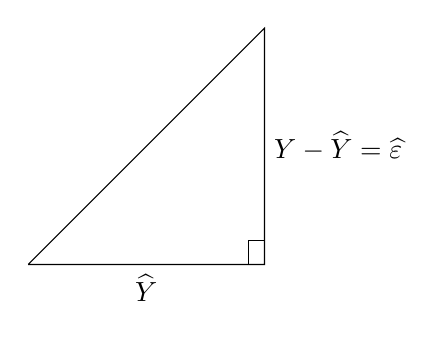
\begin{tikzpicture}[=>stealth]
\draw(0,0)--(3,0)--(3,3)--(0,0);
\draw(2.8,0)--(2.8,0.3)--(3,0.3);
\draw(3,1.5)node[right]{$Y - \widehat{Y} = \widehat{\varepsilon}$}
(1.5,0)node[below]{$\widehat{Y}$};
\end{tikzpicture}
\end{figure}





\end{enumerate}










\begin{align*}
\text{Now}\qquad   Y & = \widehat{Y} + \widehat{\varepsilon}\\
                        Y'Y & = \big(\widehat{Y}+\widehat{\varepsilon}\big)'\big(\widehat{Y}+\widehat{\varepsilon}\big)\\
                            & = \widehat{Y}'\widehat{Y} + \widehat{Y}'\widehat{\varepsilon} + \widehat{\varepsilon}'\widehat{Y} + \widehat{\varepsilon}'\widehat{\varepsilon}\\
                            & = \widehat{Y}'\widehat{Y} + 0 + 0 + \widehat{\varepsilon}'\widehat{\varepsilon}\\
                        Y'Y  & = \widehat{Y}'\widehat{Y} + \widehat{\varepsilon}'\widehat{\varepsilon}\tag{9}
\end{align*}


$Y'Y=$ Total sum of squares and cross products.\\

$\widehat{Y}'\widehat{Y}=$ Predicted sum of squares and cross products.\\

$\widehat{\varepsilon}'\widehat{\varepsilon} =$ Residual (error) sum of squares and cross products.\\


The residual sum of squares and cross products can also be written as \begin{equation}\tag{10}
\widehat{\varepsilon}'\widehat{\varepsilon} = Y'Y-\widehat{Y}'\widehat{Y}= \widehat{B}'Z'Z\widehat{B}
\end{equation}\\

\begin{exa}
Illustrate the calculations of $\widehat{B}$ and $\widehat{Y}$ and $\widehat{\varepsilon}$ we fit a straight line
\begin{align*}
y_{j1} & = \beta_{01} + \beta_{11}Z_{j1} + \varepsilon_{j1}\\
y_{j2} & = \beta_{02} + \beta_{12}Z_{j1} + \varepsilon_{j2}\qquad j=1,2,3,4,5
\end{align*}
\end{exa}



\begin{table}[H]
\centering
\begin{tabular}{c|ccccc}
$Z_1$ & 0 & 1 & 2 & 3 & 4\\
\hline
$Y_1$ & 1 & 4 & 3 & 8 & 9\\
$Y_2$ & $-1$ & $-1$ & 2 & 3 & 2\\
\end{tabular}
\end{table}


the design matrix $Z$ remains unchanged of the single respect problem.
$$ Z' =
\begin{bmatrix}
1 & 1 & 1 & 1 & 1\\
0 & 1 & 2 & 3 & 4\\
\end{bmatrix}
\qquad 
\big(Z'Z\big)^{-1}=
\begin{pmatrix}
5 & 10\\
10 & 30\\
\end{pmatrix}
$$



$$\big(Z'Z\big)^{-1} = 
\begin{pmatrix}
0.6 & -0.2\\
-0.2 & 0.1\\
\end{pmatrix}
$$\\




\begin{align*}
Z'Y_{(1)} & = 
\begin{pmatrix}
1 & 1 & 1 & 1 & 1\\
0 & 1 & 2 & 3 & 4\\
\end{pmatrix}
\begin{pmatrix}
1 \\ 4\\ 3\\ 8\\ 9\\
\end{pmatrix}\\
& = 
\begin{pmatrix}
25\\ 70\\
\end{pmatrix}\\
\end{align*}






\begin{align*}
\text{So}\qquad  \widehat{B}_{(1)} & = \big(Z'Z\big)^{-1}Z'Y_{(1)}\\
& = \begin{pmatrix}
0.6 & -0.2\\
-0.2 & 0.1\\
\end{pmatrix}
\begin{pmatrix}
25\\70\\
\end{pmatrix}\\
& = 
\begin{pmatrix}
1\\2\\
\end{pmatrix}\\\\
\end{align*}




$$Z'Y_{(2)} =
\begin{pmatrix}
1 & 1 & 1 & 1 & 1\\
0 & 1 & 2 & 3 & 4\\
\end{pmatrix}
\begin{pmatrix}
-1 \\ -1 \\ 2\\ 3\\ 2\\
\end{pmatrix}
=
\begin{pmatrix}
5\\20\\
\end{pmatrix}
$$

\begin{align*}
\text{So}\qquad  \widehat{B}_{(2)} & = \big(Z'Z\big)^{-1}Z'Y_{(2)}\\
& = \begin{pmatrix}
0.6 & -0.2\\
-0.2 & 0.1\\
\end{pmatrix}
\begin{pmatrix}
5\\ 20\\
\end{pmatrix}\\
& = 
\begin{pmatrix}
-1\\ 1\\
\end{pmatrix}\\\\
\end{align*}




\begin{align*}
\widehat{B} & = \begin{bmatrix}
\widehat{B}_{(1)} & \vdots & \widehat{B}_{(2)}\\
\end{bmatrix}\\
& = 
\begin{pmatrix}
1 & -1\\
2 & 1\\
\end{pmatrix}
=\big(Z'Z\big)^{-1}Z'Y\\
& = \big(Z'Z\big)^{-1}Z'
\begin{pmatrix}
Y_{(1)} & \vdots & Y_{(2)}\\
\end{pmatrix}\\
\end{align*}


\begin{align*}
\text{Fitted equations}\qquad  \widehat{Y}_1 & = 1 + 2Z_1\\
                                    \widehat{Y}_2 & = -1 + Z_1\\
\end{align*}




$$\widehat{Y}=Z\widehat{B}=
\begin{pmatrix}
1 & 0\\
1 & 1\\
1 & 2\\
1 & 5\\
1 & 4\\
\end{pmatrix}
\begin{pmatrix}
1 & -1\\
2 & 1\\
\end{pmatrix}
=\begin{pmatrix}
1 & -1\\
3 & 0\\
5 & 1\\
7 & 2\\
9 & 3\\
\end{pmatrix}
$$\\

 
$$\text{and}\qquad  \widehat{\varepsilon} = Y - \widehat{Y}=
\begin{pmatrix}
0 & 1 & -2 & 1 & 0\\
0 & -1 & 1 & 1 & -1\\
\end{pmatrix}'
$$\\


$$\widehat{\varepsilon}'\widehat{Y}=
\begin{pmatrix}
0 & 1 & -2 & 1 & 0\\
0 & -1 & 1 & 1 & -1\\
\end{pmatrix}
\begin{pmatrix}
1 & -1\\
3 & 0\\
5 & 1\\
7 & 2\\
9 & 3\\
\end{pmatrix}
=
\begin{pmatrix}
0 & 0\\
0 & 0\\
\end{pmatrix}
$$\\


$$Y'Y =
\begin{pmatrix}
1 & 4 & 3 & 8 & 9\\
-1 & -1 & 2 & 3 & 2\\
\end{pmatrix}
\begin{pmatrix}
1 & -1\\
4 & -1\\
3 & 2\\
8 & 3\\
9 & 2\\
\end{pmatrix}
=
\begin{pmatrix}
171 & 43\\
43 & 19\\
\end{pmatrix}
$$\\



$$\widehat{Y}'\widehat{Y}=
\begin{pmatrix}
165 & 45\\
45 & 15\\
\end{pmatrix}
\qquad \widehat{\varepsilon}'\widehat{\varepsilon}=
\begin{pmatrix}
6 & -2\\
-2 & 4\\
\end{pmatrix}
$$\\





Decomposition of sum of squares and cross-products is 
\,$Y'Y = \widehat{Y}'\hat{Y} + \widehat{\varepsilon}'\widehat{\varepsilon}$

$$
\begin{pmatrix}
171 & 43\\
43 & 19\\
\end{pmatrix}
 =
\begin{pmatrix}
165 & 45\\
45 & 15\\
\end{pmatrix} +
\begin{pmatrix}
6 & -2\\
-2 & 4\\
\end{pmatrix}
$$\\











\begin{result}
For the least squares estimates \quad $\widehat{B} = \begin{bmatrix}
\widehat{B}_{(1)} & \vdots & \widehat{B}_{(2)} & \vdots & \cdots& \widehat{B}_{(m)}\\
\end{bmatrix}
$\,
determined under the multivariate multiple regression model $()$ with full $rank(Z)=r+1<n$. $E\big(\widehat{B}_{(i)}\big) = B_{(i)}$ or $E\big(\widehat{B}\big) = B$ and $cov\big(\widehat{B}_{(i)},\widehat{B}_{(k)}\big)=\sigma_{ik}\big(Z'Z\big)^{-1},  i,k=1,2,\ldots,r+1$.\\
\end{result}

The residuals
\,$ \widehat{\varepsilon} = 
\begin{bmatrix}
\widehat{\varepsilon}_{(1)} & \vdots & \widehat{\varepsilon}_{(2)} & \vdots & \cdots& \vdots & \widehat{\varepsilon}_{(n)}\\
\end{bmatrix}
=Y-Z\widehat{B}$\,
Satisfies $E\big(\widehat{\varepsilon}_{(i)}\big)=\underline{0}$ and $E\big(\widehat{\varepsilon}_{(i)}'\widehat{\varepsilon}_{(k)}\big)=(n-r-1)\sigma_{ik}$ as a result  $E\big(\widehat{\varepsilon}\big)=0$ and $$E\Bigg(\frac{\widehat{\varepsilon}'\widehat{\varepsilon}}{n-r-1}\Bigg)=\Sigma$$


Also $\widehat{\varepsilon}$ and $\widehat{B}$ are uncorrelated.\\\\

\begin{proof}
The $i^{\text{th}}$ response follows the multiple regression model
$$Y_{(i)}=ZB_{(i)}+\varepsilon_{(i)},  E\big(\varepsilon_{(i)}\big)=\underline{0},  E\big(\varepsilon_{(i)},\varepsilon_{(i)}'\big)=\sigma_{ii}I$$
We also have:
\begin{align*}
\widehat{B}_{(i)} - B_{(i)} & = \big(Z'Z\big)^{-1}Z'Y_{(i)}-B_{(i)}\\
                        & = \big(Z'Z\big)^{-1}Z'\varepsilon_{(i)}\\
                        & = \big(Z'Z\big)^{-1}Z'\big(ZB_{(i)}+\varepsilon_{(i)}\big)-B_{(i)}\\
                        & = \big(Z'Z\big)^{-1}Z'ZB_{(i)} +\big(Z'Z\big)^{-1}Z'\varepsilon_{(i)}-B_{(i)}\\
                        & = B_{(i)} + \big(Z'Z\big)^{-1}\varepsilon_{(i)}-B_{(i)}\\
                        & = \big(Z'Z\big)^{-1}Z\varepsilon_{(i)}\\
\end{align*}
\end{proof}



\begin{align*}
\text{and}\qquad  \widehat{\varepsilon}_{(i)} & = Y_{(i)} - \widehat{Y}_{(i)}\\
                                               & = Y_{(i)} - Z\widehat{B}_{(i)}\\
                                               & = Y_{(i)} - Z\big(Z'Z\big)^{-1}Z'Y_{(i)}\\
                                               & = \big(I-Z\big(Z'Z\big)^{-1}Z'\big)Y_{(i)}\\
                                               & = \big(I-Z\big(Z'Z\big)^{-1}Z'\big)\varepsilon_{(i)}
\end{align*}


So $E\big(\widehat{B}_{(i)}=B_{(i)}$ since 
\begin{align*}
E\big(\widehat{B}_{(i)}-B_{(i)}\big) & = E\big[\big(Z'Z\big)^{-1}Z'\varepsilon_{(i)}\big]\\
                                 & = \big(Z'Z\big)^{-1}Z'\underline{0}\\
                                 & = \underline{0}\\
\end{align*}



\begin{align*}
E\big(\widehat{\varepsilon}_{(i)}\big) & = E\big[\big(I-Z\big(Z'Z\big)^{-1}Z'\big)\varepsilon_{(i)}\big]\\
                                   & = \big(I-Z\big(Z'Z\big)^{-1}Z'\big)E\big(\varepsilon_{(i)}\big)\\
                                   & = \big(I-Z\big(Z'Z\big)^{-1}Z'\big)\underline{0}\\
                                   & = \underline{0}\\
\end{align*}



Next
\begin{align*}
Cov\big(\widehat{B}_{(i)},\widehat{B}_{(k)}\big) & = E\big(\widehat{B}_{(i)}-B_{(i)}\big)\big(\widehat{B}_{(i)}-B_{(i)}\big)'\\
& = E\big[\big(Z'Z\big)^{-1}Z'\varepsilon_{(i)}\varepsilon'_{(k)}Z\big(Z'Z\big)^{-1}\big]\\
& = \big(Z'Z\big)^{-1}Z'\sigma_{ik}IZ\big(Z'Z\big)^{-1}\\
& = \sigma_{ik}\big(Z'Z\big)^{-1}Z'Z\big(Z'Z\big)^{-1}\\
& = \sigma_{ik}\big(Z'Z\big)^{-1}\\
\end{align*}



If $\underline{U}$ is any random vector and $A$ is a fixed matrix then
\begin{align*}
E\big(U'AU\big) & = E\big(tr\big(U'AU\big)\big)\\
                & = E\big(tr(AUU'\big)\big)\\
                & = tr\big(AE\big(UU'\big)\big)
\end{align*}

Using this result we have
\begin{align*}
E\big(\widehat{B}_{(i)}',\widehat{B}_{(k)}\big) & = E\big(\varepsilon'_{(i)}\big(I-Z\big(Z'Z\big)^{-1}Z'\big)\varepsilon_{(k)}\big)\\
& = tr\big[\big(I-Z\big(Z'Z\big)^{-1}Z'\big)\sigma_{ik}I\big]\\
& = \sigma_{ik}tr\big(I-Z\big(Z'Z\big)^{-1}Z'\big)\\
& = \sigma_{ik}\big[tr(I)-tr\big(Z\big(Z'Z\big)^{-1}Z'\big]\\
& = \sigma_{ik}\big(n-tr\big[\big(Z'Z\big)^{-1}Z'Z\big]\\
& = \sigma_{ik}\big(n-tr I_{r+1}\big)\\
& = \sigma_{ik}\big(n-(r+1)\big)\\
& = \sigma_{ik}(n-r-1)\\
\end{align*}

dividing each entry  $\widehat{\varepsilon}_{(i)}'\widehat{\varepsilon}_{(k)}$ of $\widehat{\varepsilon}'\widehat{\varepsilon}$ by $n-r-1$, we obtain the unbiased estimate of $\Sigma$. Finally $\big(\widehat{\varepsilon}_{(i)},\widehat{\varepsilon}_{(k)}\big) = E\big[\big(Z'Z\big)^{-1}Z'\varepsilon_{(i)}\varepsilon_{(k)}'H\big]$ where 
\begin{align*}
H &  = I- Z\big(Z'Z\big)^{-1}Z'\\
  & = \big(Z'Z\big)^{-1}Z'\big(\varepsilon_{(i)}\varepsilon_{(k)}'\big)\big(I-Z\big(Z'Z\big)^{-1}Z'\big)\\
  & = \big(Z'Z\big)^{-1}Z'\sigma_{ik}I\big(I-Z\big(Z'Z\big)^{-1}Z'\big)\\
  & = \sigma_{ik}\big(Z'Z\big)^{-1}Z'-\sigma_{ik}\big(Z'Z\big)^{-1}Z'Z\big(Z'Z\big)^{-1}Z'\\
  & = \sigma_{ik}\big(\big(Z'Z\big)^{-1}Z'-\big(Z'Z\big)^{-1}Z'\big)\\
  & = 0
\end{align*}

each elements of $\widehat{B}$ is uncorrelated with each element of $\widehat{\varepsilon}$.


% DIAGRAM 13

\begin{figure}[H]
\centering
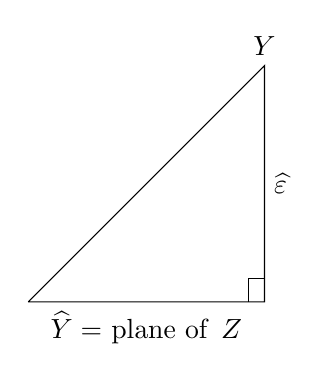
\begin{tikzpicture}[=>stealth]
\draw(0,0)--(3,0)--(3,3)--(0,0);
\draw(2.8,0)--(2.8,0.3)--(3,0.3);
\draw(3,1.5)node[right]{$ \widehat{\varepsilon}$}
(1.5,0)node[below]{$\widehat{Y}=$ plane of $\,Z$}
(3,3)node[above]{$Y$};
\end{tikzpicture}
\end{figure}











the mean vectors and Covariance matrices determined in result 1 enables us to predict sampling properties of the least squares predictors.\\\\






\begin{center}
\textbf{SAMPLING PROPERTIES}
\end{center}
\textbf{Introduction:}\\
We first consider the problem of estimating the mean vector were the predictor variable, us values
$$Z_0 =
\begin{bmatrix}
1 & Z_{01} & \cdots Z_{0r}\\
\end{bmatrix}'
$$ 
then mean of $i^{\text{th}}$ response variable is $Z_0'B_{(i)1}$ , and this is estimated by $\widehat{Z}_0B_{(i)1}$  the $i^{\text{th}}$ component of the fitter relationship. Collectively
\begin{equation}\tag{11}
Z_0'\widehat{B} =
\begin{bmatrix}
Z_0'\widehat{B}_{(i)} & \vdots & Z_0'\widehat{B}_{(2)} & \vdots & \cdots& \vdots & Z_0'\widehat{B}_{(m)}\\
\end{bmatrix}'
\end{equation}
is unbiased estimator of $Z_0'\widehat{B}$
$$E\big(Z_0'\widehat{B}_{(i)}\big) = Z_0'E\big(\widehat{B}_{(i)}\big) = Z_0'B_{(i)}\qquad\text{for each component}$$


Using the Covarince matrix for $\widehat{B}_{(i)}$ and $\widehat{B}_{(k)}$ the estimation errors $Z'_0B_{(i)}-Z_0'\widehat{B}_{(i)}$ have covariances


\begin{align*}
E\big[Z'_0\big(B_{(i)}-\widehat{B}_{(i)}\big)\big(B_{(k)}-\widehat{B}_{(k)}\big)'Z_0\big] & = Z_0'\big(E\big(B_{(i)}-\widehat{B}_{(i)}\big)\big(B_{(k)}-\widehat{B}_{(k)}\big)'\big)Z_0\\
& = Z_0'\big(\sigma_{ik}\big(Z'Z\big)^{-1}\big)Z_0\\
& = \underbrace{\sigma_{ik}Z_0'\big(Z'Z\big)^{-1}Z_0}_{(r+1)\times (r+1)}\tag{12}\\
\end{align*}




The related problem is that of forecasting the new observation vector $Y_0 =
\begin{bmatrix}
Y_{01}, & Y_{02}, & \cdots, & Y_{0m}\\
\end{bmatrix}'
$ at $Z_0$.\\

According to the regression model $\, Y_{0i} = Z'_{0}B_{(i)} + \varepsilon_{oi}\,$ where the ``new" error\\ $\varepsilon_0 = 
\begin{bmatrix}
\varepsilon_{01},& \varepsilon_{02}, & \cdots, \varepsilon_{0m}\\
\end{bmatrix}'$ is independent of the error $\varepsilon$ and satisfies $E\big(\varepsilon_{0i}\big)=0$ and $E\big(\varepsilon_{0i},\varepsilon_{0k}\big)=\sigma_{ik}$.\\


The forecast error for the $i^{\text{th}}$ component of $Y_0$ is 
\begin{align*}
Y_{0i} - Z'_0\widehat{B}_{(i)} &  = Y_{0i} - Z_0'B_{(i)} + Z'_{0}B_{(i)} - Z_0'\widehat{B}_{(i)}\\
                           & = \varepsilon_{0i} - Z_0'\big(\widehat{B}_{(i)}-B_{(i)}\big)
\end{align*}


\begin{align*}
\text{So}\quad  E\big(Y_{0i}-Z'_0\widehat{B}_{(i)}\big) & = E\big(\varepsilon_{0i}\big)-E\big(Z_0'\big(\widehat{B}_{(i)}-B_{(i)}\big)\big)\\
& = 0 - Z'_0 E\big(\widehat{B}_{(i)}-B_{(i)}\big)\\
& = 0- Z'_0\cdot 0\\
& = 0
\end{align*}

Indicating $Z_0'\widehat{B}_{(i)}$ is unbiased predictor of $Y_{0i}$.\\

The forecasts errors have covariances
\begin{align*}
E\big(Y_{0i}-Z_0'\widehat{B}_{(i)}\big)\big(Y_{0k}-Z'_0\widehat{B}_{(k)}\big) & = E\big(\varepsilon_{0i}-Z'_0\big(\widehat{B}_{(i)}-B_{(i)}\big)\big)\big(\varepsilon_{(0k)}-Z'_0\big(\widehat{B}_{(k)}-B_{(k)}\big)\big)\\
& = E\big(\varepsilon_{0i}\varepsilon_{0k}\big) + Z'_0E\big(\widehat{B}_{(i)}-B_{(i)}\big)\big(\widehat{B}_{(k)}-B_{(k)}\big)'Z_0-Z_0'E\big(\big(\widehat{B}_{(i)}-B_{(i)}\big)\varepsilon_{0k}\big)\\
& - E\big(\varepsilon_{0i}\big(\widehat{B}_{(k)}-B_{(k)}\big)\big)Z_0\\
& = \sigma_{ik}+Z_0'\sigma_{ik}\big(Z'Z\big)^{-1}Z_0+Z_0'\cdot 0-0\cdot Z_0\\
& = \sigma_{ik}\big(1+Z_0\big(Z'Z\big)^{-1}Z_0\big)\\  
\end{align*}


Note that $E\big(\big(\widehat{B}_{(i)}-B_{(i)}\big)\varepsilon_{0k}\big)=0$ since $\widehat{B}_{(i)}=\big(Z'Z\big)^{-1}Z'\varepsilon_{(i)}+B_{(i)}$.
is independent of $\varepsilon_0$ future (error) while $\varepsilon_{(i)}$ is a  present error.\\

A similar result holds for $E\big(\varepsilon_{0i}\big(\widehat{B}_{(k)}-B_{(k)}\big)$.\\\\


Maximum likelihood estimators and their distributions can be obtained everywhere the errors $\varepsilon$ have normal distribution.\\

\begin{result}
Let the multivariate regression model (1) hold with full rank. $rank (Z) = r+1,\\ n\geq (r+1)+m$\, and that the errors $\varepsilon$ have a normal distribution. Then \,$\widehat{B}=\big(Z'Z\big)^{-1}Z'Y.\,$ Maximum likelihood estimator of $B$ and $\widehat{B}$ has a normal distribution with $E\big(\widehat{B}=B\big)$ and $Cov\big(\widehat{B}_{(i)},\widehat{B}_{(k)}\big)=\sigma_{ik}\big(Z'Z\big)^{-1}$. Also $\widehat{B}$ is independent of the maximum likelihood estimator positive definite given by $$\widehat{\Sigma}=\frac{\widehat{\varepsilon}'\widehat{\varepsilon}}{n}=\big(Y-Z\widehat{B}\big)\big(Y-Z\widehat{B}\big)$$ and $\displaystyle{n\widehat{\Sigma}}$ is distributed as $W_{n-r-1}\quad  \Big(\cdot \big|\displaystyle{\Sigma}\big|\Big)$.\\\\
\end{result}




\begin{proof}
According to regression model, the likelihood is determined from the data $Y=
\begin{bmatrix}
y_1 & y_2 & \cdots& y_n\\
\end{bmatrix}'
$ whose roots are independent with $y_i$ distributed as $N_m\big(B'Z_j,\displaystyle{\Sigma}\big)$. We first note that 
$$ y-ZB = 
\begin{bmatrix}
y_1-B'Z_1, & y_2-B'Z_2, & \cdots, & y_n-B'Z_n\\
\end{bmatrix}'
$$ So
\,$\displaystyle{\big(y-ZB\big)'\big(y-ZB\big)=\sum^n_{j=1}\big(y_j-B'Z_j\big)\big(y_j-B'Z_j\big)'}\,$
and 
\begin{align*}
\sum^n_{j=1}\big(y_j-B'Z_j\big)'\Sigma^{-1}\big(y_j-B'Z_j\big) & = \sum^n_{j=1}tra\Big[\big(y_j-B'Z_j\big)'\Sigma^{-1}\big(y_j-B'Z_j\big)\Big]\\
&= tra\Big[\Sigma^{-1}\big(Y-ZB\big)'\big(Y-ZB\big)\Big]\tag{1}
\end{align*}
\end{proof}



Another preliminary calculation will enable us to express the likelihood in a simple form.\\
Since $\widehat{\varepsilon}=Y-Z\hat{B}$ satisfies $Z'\widehat{\varepsilon}=0$. Then 
\begin{align*}
\big(Y-ZB\big)'\big(Y-ZB\big) & = \Big[Y-Z\widehat{B}+Z\big(\widehat{B}-B\big)\Big]\Big[Y-Z\widehat{B}+Z\big(\widehat{B}-B\big)\Big]\\
& = \big(Y-Z\widehat{B}\big)'\big(Y-Z\widehat{B}]\big) + \big(\widehat{B}-B\big)'ZZ'\big(\widehat{B}-B\big)\\
& = \widehat{\varepsilon}'\widehat{\varepsilon} + \big(\widehat{B}-B\big)'Z'Z\big(\widehat{B}-B\big)\tag{2}
\end{align*}

Using (1) and (2) we obtain the likelihood
\begin{align*}
L\big(B,\Sigma\big) & = \prod^n_{j=1}\frac{1}{\big(2\pi\big)^{m/2}}\frac{1}{\big|\Sigma\big|^{1/2}}\exp\Big\{-\frac{1}{2}\big(y_i-B'Z_j\big)'\Sigma^{-1}\big(y_j-B'Z_j\big)\Big\}\\
& = \frac{1}{\big(2\pi\big)^{nm/2}}\cdot \frac{1}{\big|\Sigma\big|^{n/2}}\exp\Big\{-\frac{1}{2}tra\Big[\Sigma^{-1}\big(\widehat{\varepsilon}'\widehat{\varepsilon}+\big(\widehat{B}-B\big)'Z'Z\big(\widehat{B}-B\big)\big)\Big]\Big\}\\
& = \frac{1}{\big(2\pi\big)^{nm/2}}\cdot\frac{1}{\big|\Sigma\big|^{n/2}}\exp\Big\{-\frac{1}{2}tra\Big(\Sigma^{-1}\widehat{\varepsilon}'\widehat{\varepsilon}\Big)-\frac{1}{2}tra\Big[Z\big(\widehat{B}-B\big)\Sigma^{-1}\big(\widehat{B}-B\big)'Z'\Big]\Big\}
\end{align*}


The matrix $Z\big(\widehat{B}-B\big)\Sigma^{-1}\big(\widehat{B}-B\big)'Z'$ is of the form \,$\displaystyle{A=\Sigma^{-\frac{1}{2}}\big(\widehat{B}-B\big)'Z'}\,$ is non-negative definite. The trace \,$\displaystyle{tra\big(Z\big(\widehat{B}-B\big)\Sigma^{-1}\big(\widehat{B}-B\big)'Z'\big)}\,$ is the sum of its eigenvalues, this trace will equal its maximum value 0 if $\widehat{B}=B$. This choice is unique because $Z$ is of full rank.\\
Applying an earlier result with $B=\widehat{\varepsilon}'\widehat{\varepsilon},  b=\frac{n}{2}$ and $p=m$, we find that $\widehat{B}$ and $\displaystyle{\widehat{\Sigma}=\frac{\widehat{\varepsilon}'\widehat{\varepsilon}}{2}}$ are the $MLE$ of $B$ and $\displaystyle{\Sigma}$, respectively , and 
\begin{equation}\tag{3}
L\big(\widehat{B},\widehat{\Sigma}\big) = \frac{1}{\big(2\pi\big)^{nm/2}}\cdot\frac{n^{nm/2}}{\big|\widehat{\varepsilon}'\widehat{\varepsilon}\big|^{n/2}}e^{-nm/2}=\frac{e^{-nm/2}}{\big(2\pi\big)^{nm/2}\big|\hat{\Sigma}\big|^{n/2}}
\end{equation}




It remains to establish the distribution results $\widehat{B}_{(i)}$ and $\widehat{\varepsilon}_{(i)}$ are linear combinations of elements of $\varepsilon$. Specifically
\begin{align*}
\widehat{B}_{(i)} & = \big(Z'Z\big)^{-1}Z'\varepsilon_{(i)} + B_{(i)}\\
\widehat{\varepsilon}_{(i)} & = \big[I- Z\big(Z'Z\big)^{-1}Z'\big]\varepsilon_{(i)},  i=1,2,\ldots,m
\end{align*}

Therefore, $\widehat{B}_{(1)}, \widehat{B}_{(2)},\ldots,\widehat{B}_{(m)}, \widehat{\varepsilon}_{(1)},\ldots, \widehat{\varepsilon}_{(m)}$ are jointly normal.\\
There mean vectors and covariances are given in equation (1) result (1).\\
Since $\widehat{\varepsilon}$ and $\widehat{B}$ have zero covariance matrix, there are independent.\\

Further we have the following $I-Z\big(Z'Z\big)^{-1}Z'=\sum\limits^{n-r-1}_{l=1}\underline{e}_l\underline{e}_l'$ where $\underline{e}_l'\underline{e}_k=0$ for $l\neq k$. and $\underline{e}'_l\underline{e}_l=1$. Let
\begin{align*}
V_l & = \Sigma'\underline{e}_l= \begin{bmatrix}
\varepsilon'_{(1)}e_l, & \varepsilon'_{2}e_l, & \cdots, & \varepsilon'_{n}e_l\\
\end{bmatrix}\\
& = e_{l_1}\varepsilon_1 + e_{l_2}\varepsilon_2 + \cdots+ e_{l_n}\varepsilon_n
\end{align*}



Because $V_l, l=1,2,\ldots, n-r-1$ are linear combinations of $\varepsilon$ , there have a joint normal distribution with $E\big(V_l\big) = E\big(\varepsilon'\underline{e}_l\big)$ also form our previous layout have covariance matrix $V_l$  and $V_k$
$$\big(e'_le_k\big) = 0\cdot\big(\Sigma\big) =0\qquad \text{if}\quad  l\neq k$$

Consequently the independent $l's$ are evenly distributed as $N_m\big(0,\Sigma\big)$. Finally 
\begin{align*}
\widehat{\varepsilon}'\widehat{\varepsilon} & = \varepsilon' \big[I- Z\big(Z'Z\big)^{-1}Z'\big]\varepsilon\\
& = \sum^{n-r-1}_{\rho=1}\varepsilon'e_le'_l\varepsilon\\ &
 = \sum^{n-r-1}_{\rho=1} V_lV_l'
\end{align*}

Whishart distribution $W_{n-r-1}\Big(\cdot , \Sigma\Big)\equiv W_m\Big(n-r-1,\Sigma\Big)$\\\\








\begin{center}
\textbf{INFERENCE}
\end{center}
Likelihood Ratio Tests for Regression Parameters.\\

In multiple response analog of univariate response model the hypothesis that the responses do not dependent on $Z_{q+1}, Z_{q+2}, \ldots, Z_r$ becomes $H_0: B_{(2)} =B = 0$ where\\ $B = \begin{bmatrix}
B_{(1)_{(q\times 1)\times m}}\\
\cdots\\
B_{2_{(l-q)\times m}}\\
\end{bmatrix}$ setting 
$Z=
\begin{bmatrix}
Z_1 & \vdots & Z_2\\
n\times (q+1) & \vdots & n\times (n-q)\\
\end{bmatrix}$ the general model  becomes
$$E(Y)=
\begin{bmatrix}
Z_1 & \vdots & Z_2\\
\end{bmatrix}
\begin{bmatrix}
B_{(1)}\\
\cdots\\
B_{(2)}\\
\end{bmatrix}
=Z_1B_{(1)} + Z_2B_{(2)}$$
Under $H_0: B_{(2)} = 0$ \\
$Y= Z_1B_{(1)} + \varepsilon$  and the likelihood ratio test of $H_0$ is based on the quantities involved in the extra sum of squares and cross-products
$$\big(Y-Z_1\widehat{B}_{(1)}\big)'\big(Y-Z_1\widehat{B}_{(1)}\big) - \big(Y-Z\widehat{B}\big)'\big(Y-Z\widehat{B}\big)=n\big(\widehat{\Sigma}_1-\widehat{\Sigma}\big)$$
where $\widehat{B}_{(1)}=\big(Z_1'Z_1\big)^{-1}Z'_1Y$ and $\sum\limits^n_l=\big(Y-Z_l\widehat{B}_{(l)}\big)'\big(Y-Z_l\widehat{B}_{(l)}\big)/n$.\\
The likelihood ratio can be expressed of generalized variances so




\begin{align*}
\Delta & = \frac{\max\limits_{B_{(i)},\Sigma}L\big(B_{(i)},\Sigma\big)}{\max\limits_{B,\Sigma}L\big(B,\Sigma\big)}
         = \frac{L\Big(\widehat{B}_{(i)},\widehat{\Sigma}_{(i)}\Big)}{L\Big(\widehat{B},\widehat{\Sigma}\Big)}\\\\
       & = \Bigg(\frac{\big|\widehat{\Sigma}\big|}{\big|\widehat{\Sigma}_l\big|}\Bigg)^{\frac{n}{2}}
\end{align*}
equivalent Wilk's Lambda statistic $\Delta^{2/n}=\frac{\big|\widehat{\Sigma}\big|}{\big|\widehat{\Sigma}_l\big|}$ can be used.\\\\


\begin{result}
Let the multivariate multi regression model (1) hold with $Z$ of full rank $r+1$ and $(r+1)+m<n$. Let the error $\varepsilon$ be normally distributed under $H_0: B_{(2)} =0$.\\
$n\widehat{\Sigma}\thicksim W_m\big(n-r-1, \Sigma\big)$ independent of $n\big(\widehat{\Sigma}_l-\widehat{\Sigma}\big)$ which in turn $n\big(\widehat{\Sigma}_l-\widehat{\Sigma}\big)\thicksim W_m\big(r-q,\Sigma\big)$.\\
\end{result}

The likelihood ratio test of $H_0$ is equivalent to rejection $H_0$ for large values of 
\begin{align*}
-2\ln \Delta & = -n\ln \Bigg(\frac{\big|\widehat{\Sigma}\big|}{\big|\widehat{\Sigma}_l\big|}\Bigg)\\\
& = -n\ln \frac{n\widehat{\Sigma}}{\Big|n\widehat{\Sigma}+n\big(\widehat{\Sigma}_l-\widehat{\Sigma}\big)\Big|}
\end{align*}

for large $n$ the modified statistic is 
$$-\big[n-r-1-\frac{1}{2}(m-r+q+1)\big]\ln \Bigg(\frac{\big|\widehat{\Sigma}\big|}{\big|\widehat{\Sigma}_l}\Bigg)$$

has a close to approximation a Chi-square distribution. i.e $\thicksim \chi^2_{m(r-q)}$.\\\\



\begin{exa}
The services in three locations of a large restaurant chain was rated according to the majors by male and female patrons.\\
\end{exa}

Suppose we consider a regression under that allows for the effects and the location gender interrelation services quality indexes.\\
A computer program provides the following

$$\begin{pmatrix}
\text{Residual sum of}\\
\text{squares and cross}\\
\text{-products}\\
\end{pmatrix}= n\widehat{\Sigma}=
\begin{pmatrix}
2977.39 & 1021.72\\
1021.72 & 2050.95\\
\end{pmatrix}$$\\


$$\begin{pmatrix}
\text{Extra sum of }\\
\text{squares and }\\
\text{cross-products}\\
\end{pmatrix}=n\big(\widehat{\Sigma}-\Sigma\big)=
\begin{pmatrix}
441.76 & 246.16\\
246.16 & 364.12\\
\end{pmatrix}$$



Let $B_2$ be the matrix of interrelationships presentation for the two responses although the sample size $n=18$ is not large we shall illustrate the calculation involved in the test of $B_{(2)} = 0 $ setting $\alpha = 0.05$ we set $H_0$ by referring
\begin{align*}
&-\big[n-r_1-1-\frac{1}{2}(m-r_1+q_1+1)\big]\times \ln \frac{\big|n\widehat{\Sigma}\big|}{\Big|n\widehat{\Sigma}+n\big(\widehat{\Sigma}_l-\widehat{\Sigma}\big)\Big|}\\\\
& = -\big[18 - 5 -1 -\frac{1}{2}(2-5+3+1)\big]\ln (0.7605)\\
& = 3.28\qquad \text{to a Chi-square}
\end{align*}
$$n(r_1-q_1)=2(2) = 4 df$$
Since $3.28 < \chi^2_{4,(0.05)}= 9.49$, we fail to reject $H_0$\\
Interrelation term not needed.\\\\





\begin{center}
\textbf{Other Tests}
\end{center}
Tests other than the likelihood ratio have been proposed for the multivariate multiple model. The most prominent alternative is the Roy's greatest Root which rejects $H_0:_{\eta}B_{(2)}=\underline{0}$ for where $\eta$ is the greater root of $$\Bigg|\Big(\widehat{\Sigma}_l-\widehat{\Sigma}\Big)-\eta \widehat{\Sigma}\Bigg| = 0\qquad\text{Polynomial of order }m$$
 tables of critical values are available for quantities \,$\displaystyle{U=\frac{\eta}{1 + \eta}}\,$ critical value of $\eta_{\alpha}$ are given $$\eta_{\alpha} = \frac{\theta_{\alpha}}{1- \theta_{\alpha}}$$
 
 
Hotellings-Lawley Trace test is based on the the sum of the roots $\eta$.\\

Wilk's Lambda, Roy's Greatest Root and Hotelling - Lawley are nearly equivalent for large sample sizes.\\\\




\begin{center}
\textbf{Predictions for Multivariate Multiple Regression}
\end{center}
Suppose the model $Y= ZB + \varepsilon$ with normal errors $\varepsilon$ has been fitted and checked for any inadequacies.\\ If the model is adequate it can be employed for predication purpose.\\
One problem is to predict the mean responses corresponding to fixed $Z_0$.\\
Inference about the mean response can be made using the distribution theory using result 2.\\


From this result we determine $\widehat{B}'Z_0$ is distributed as $N_m\big(B'Z_0,Z_0'\big(Z'Z\big)^{-1}Z_0\Sigma\big)$ and $n\widehat{\Sigma}$ is independently distributed as $W_m\big(n-r-1,\Sigma\big)$.\\

Then unknown value of the regression  function at $Z_0$ is $B'Z_0$ so from the discussion of the Hotellings - $T^2$ we write
\begin{equation}\tag{4}
T^2 = \Bigg(\frac{\widehat{B}'Z_0-B'Z_0}{\sqrt{\Big(Z'_0\big(Z'Z\big)^{-1}Z_0\Big)}}\Bigg)'\Bigg(\frac{n\widehat{\Sigma}}{n-r-1}\Bigg)^{-1} \Bigg(\frac{\widehat{B}'Z_0-B'Z_0}{\sqrt{Z_0'\big(Z'Z\big)^{-1}Z_0}}\Bigg)
\end{equation} and the $100(1-\alpha)\%$ confidence ellipsoid for $B'Z_0$ is provided by the inequality 

\begin{align*}
\big(B'Z_0-\widehat{B}'Z_0\big)'\Bigg(\frac{n\widehat{\Sigma}}{n-r-1}\Bigg)^{-1}\big(B'Z_0-\widehat{B}'Z_0\big) \leq Z_0'\big(Z'Z\big)^{-1}Z_0\Bigg[\Bigg(\frac{m(n-r-1)}{n-r-m}\Bigg)F_{m,n-r-m}(\alpha)\Bigg]
\end{align*}
where $F_{m,n-r-m}(\alpha)$ is the upper $(100 \alpha^{\text{th}})$ percentile of an $F-$ distribution with $m$ and $n-r-m$ $df$.\\

The $100(1-\alpha)\%$ simultaneous confidence intervals for \,$E(Y_i)   = Z_0'B_{(i)}$

\begin{align*}
Z_0'\widehat{B}_{(i)} & \pm \sqrt{\Bigg(\frac{m(n-r-1)}{n-r-m}\Bigg)F_{m,n-r-m}(\alpha)}\times \sqrt{Z_0'\big(Z'Z\big)^{-1}Z_0\Bigg(\frac{n}{n-r-1}\Bigg)\widehat{\sigma}_{ii}}
\end{align*}






where $\widehat{B}_{(i)}$ is the $i^{\text{th}}$ column of $\widehat{B}$ and $\widehat{\sigma}_{ii}$ is the $i^{\text{th}}$ diagonal element of $\widehat{\Sigma}$.\\

































\pagebreak
\begin{thebibliography}{}
\bibitem{AA}
Applied Multivariate Statistical Analysis; Richard A Johnson and Dean W Wichem; Prentice Hall; ISBN 0-13-092553-5
\bibitem{BB}
Introduction to Multivariate Analysis; C. Chatfield and A.J.Collins; Chapman and Hall; ISBN 0 412 16040 4
\end{thebibliography}



\newpage

\subsection{Practice Problems}

\begin{problem}
Write the multivariate regression model $Y = ZB + \varepsilon$ in full,
identifying the dimensions of every matrix, and state the assumptions on
$\varepsilon$.
\end{problem}

\begin{problem}
Show that the least squares estimator is
$\widehat{B} = \left(Z'Z\right)^{-1}Z'Y$, and that each column of $\widehat{B}$
is exactly the univariate least squares estimator obtained by regressing the
corresponding response on $Z$ alone.
\emph{Where to start: minimise $\operatorname{tr}\left[(Y-ZB)'(Y-ZB)\right]$,
and note that it separates into a sum over the columns.}
\end{problem}

\begin{solution}
Writing the trace as a sum over responses,
$$\operatorname{tr}\left[(Y-ZB)'(Y-ZB)\right]
= \sum^{m}_{i=1}\left(\underline{y}_{(i)}-Z\underline{b}_{(i)}\right)'
\left(\underline{y}_{(i)}-Z\underline{b}_{(i)}\right),$$
in which the $i$th term involves only the $i$th column of $B$. The sum is
therefore minimised by minimising each term separately, which is the ordinary
least squares problem for that response, giving
$\widehat{\underline{b}}_{(i)} = (Z'Z)^{-1}Z'\underline{y}_{(i)}$ and hence
$\widehat{B} = (Z'Z)^{-1}Z'Y$.

This is worth noticing: the point estimates gain nothing from being computed
jointly. What the multivariate treatment adds is the covariance structure
between responses, which is what tests and confidence regions depend on.
\end{solution}

\begin{problem}
Show that the residual matrix $\widehat{\varepsilon} = Y - Z\widehat{B}$
satisfies $Z'\widehat{\varepsilon}=0$, and interpret this geometrically.
\end{problem}

\begin{problem}
Given the result of the second problem, explain why a multivariate regression
is nevertheless worth performing rather than $m$ separate regressions.
\end{problem}

\begin{problem}
Show that $\widehat{\Sigma} = \tfrac{1}{n}\widehat{\varepsilon}'\widehat{\varepsilon}$
is biased and that dividing instead by $n-r-1$, where $r+1$ is the number of
columns of $Z$, removes the bias.
\end{problem}

\section{Factor Analysis}

Principal component analysis in Section~4 rewrote $p$ variables as $p$
uncorrelated components and then discarded the smaller ones. It is a
transformation of the data, and it proposes no explanation of them.

Factor analysis proposes one. It supposes that the observed variables are
correlated \emph{because} they are driven by a small number of unobserved
quantities, and it asks what those quantities would have to look like. The two
methods are often confused, produce similar-looking output, and answer different
questions.

\subsection{The Orthogonal Factor Model}

\begin{defn}[Factor model]
The vector $\underline{X}$ with mean $\underline{\mu}$ follows the
\emph{$m$-factor model} if
$$\underline{X}-\underline{\mu} = L\,\underline{F} + \underline{\varepsilon},$$
where $L$ is the $p\times m$ matrix of \emph{loadings}, $\underline{F}$ is the
$m\times1$ vector of \emph{common factors} and $\underline{\varepsilon}$ the
$p\times1$ vector of \emph{specific factors}, with
$$E(\underline{F}) = \underline{0},\quad
\operatorname{cov}(\underline{F}) = I_m,\quad
E(\underline{\varepsilon}) = \underline{0},\quad
\operatorname{cov}(\underline{\varepsilon}) = \Psi
= \operatorname{diag}(\psi_1,\dots,\psi_p),$$
and $\underline{F}$ independent of $\underline{\varepsilon}$.
\end{defn}

\begin{thm}[The covariance structure]
\label{thm:factorcov}
Under the factor model,
$$\Sigma = LL' + \Psi,$$
so that
$$\sigma_{ii} = \underbrace{\ell_{i1}^{2}+\cdots+\ell_{im}^{2}}_{\text{communality } h_i^{2}}
+ \underbrace{\psi_i}_{\text{specific variance}},
\qquad
\sigma_{ik} = \sum^{m}_{j=1}\ell_{ij}\ell_{kj} \ \ (i\neq k).$$
\end{thm}

\begin{note}
The second equation is the whole content of the model, and it is a strong
claim: \emph{all} the covariance between distinct variables is carried by the
common factors, since $\Psi$ is diagonal and contributes nothing off the
diagonal. If the model holds with small $m$, the $\binom{p}{2}$ covariances are
generated by only $pm$ loadings, which is a genuine and testable reduction.

The variance of each variable splits into the part explained by the common
factors, its communality, and the part specific to it. A variable with low
communality is not being described by the factors at all, and its presence in
the analysis should be reconsidered.
\end{note}

\begin{note}[Why this is not principal component analysis]
Three differences, in order of importance.

Principal components are defined as linear combinations \emph{of} the observed
variables; factors are hypothesised causes \emph{of} them, and the arrows point
the other way. Principal components always exist and are unique; a factor model
with a given $m$ may fit no covariance matrix at all, so factor analysis can
fail in a way that principal component analysis cannot. And principal components
account for total variance, including each variable's specific noise, while
factor analysis explicitly sets that noise aside in $\Psi$ and models only what
is shared.
\end{note}

\subsection{Non-uniqueness and Rotation}

\begin{thm}[Rotational indeterminacy]
\label{thm:rotation}
If $T$ is any $m\times m$ orthogonal matrix, then $L^{*}=LT$ and
$\underline{F}^{*}=T'\underline{F}$ satisfy the model with the same $\Psi$, and
$$L^{*}L^{*\prime} = LTT'L' = LL'.$$
\end{thm}

\begin{note}
The loadings are therefore determined only up to an orthogonal rotation: the
data cannot distinguish $L$ from $LT$, whatever $T$ may be. This is an
embarrassment and an opportunity in equal measure. It is an embarrassment
because no rotation is more correct than another, so any claim that the factors
have been identified must be read carefully. It is an opportunity because one
may as well choose the rotation that is easiest to interpret --- which is what
\emph{varimax} does, seeking loadings near $0$ or $\pm1$ so that each variable
loads heavily on one factor and negligibly on the rest.

Interpretation of rotated factors is the part of multivariate analysis where
judgement most easily outruns evidence. The rotation was chosen for
interpretability; that the result is interpretable is therefore not evidence
that it is true.
\end{note}

\subsection{Estimation}

Two methods are standard.

The \emph{principal factor} method estimates the communalities, subtracts the
resulting $\widehat{\Psi}$ from $S$ or $R$, and takes the spectral decomposition
of the remainder, setting
$\widehat{L} = \left(\sqrt{\widehat{\lambda}_1}\widehat{\underline{e}}_1,
\dots,\sqrt{\widehat{\lambda}_m}\widehat{\underline{e}}_m\right)$. It requires
no distributional assumption and always produces an answer.

The \emph{maximum likelihood} method assumes $\underline{X}$ multivariate normal
and maximises the likelihood over $L$ and $\Psi$ subject to a uniqueness
condition that removes the rotational freedom. It is iterative, may fail to
converge, and can return a \emph{Heywood case} --- an estimated specific
variance that is zero or negative, which is impossible and signals that the
model with that $m$ does not fit. Against these drawbacks it offers what the
other method cannot: a likelihood ratio test of the adequacy of $m$ factors,
$$-2\ln\Lambda = \left(n-1-\tfrac{2p+4m+5}{6}\right)
\ln\frac{\left|\widehat{L}\widehat{L}'+\widehat{\Psi}\right|}{\left|S\right|}
\ \overset{\cdot}{\sim}\ \chi^{2}_{\left[(p-m)^{2}-p-m\right]/2}.$$

\begin{note}
The degrees of freedom are worth reading rather than copying. They count
$\tfrac12 p(p+1)$ free entries in $\Sigma$ against $pm+p$ parameters, less the
$\tfrac12 m(m-1)$ constraints imposed to fix the rotation. When the count is
negative the model has more parameters than the covariance matrix has entries
and cannot be tested at all --- which places a hard upper limit on $m$ for a
given $p$, independent of any data.
\end{note}

\newpage

\subsection{Practice Problems}

\begin{problem}
State two differences between principal component analysis and factor analysis,
and give a situation in which each would be the appropriate choice.
\end{problem}

\begin{problem}
For a one-factor model with $p=3$, write $\Sigma=LL'+\Psi$ in full and count the
free parameters against the entries of $\Sigma$. Is the model testable?
\emph{Where to start: $\Sigma$ has $\tfrac12 p(p+1)=6$ distinct entries; the
model has $pm+p=6$ parameters.}
\end{problem}

\begin{solution}
With $m=1$, $L=(\ell_1,\ell_2,\ell_3)'$ and
$\Psi=\operatorname{diag}(\psi_1,\psi_2,\psi_3)$, so
$$\Sigma = \begin{pmatrix}
\ell_1^{2}+\psi_1 & \ell_1\ell_2 & \ell_1\ell_3\\
\ell_1\ell_2 & \ell_2^{2}+\psi_2 & \ell_2\ell_3\\
\ell_1\ell_3 & \ell_2\ell_3 & \ell_3^{2}+\psi_3
\end{pmatrix}.$$
There are $6$ parameters and $6$ distinct entries, and with $m=1$ the
rotational constraint count $\tfrac12 m(m-1)$ is zero. The degrees of freedom
are $6-6=0$: the model is exactly determined, fits any $\Sigma$ with the right
sign pattern, and there is nothing to test. Testability needs
$\tfrac12\left[(p-m)^{2}-p-m\right]>0$, which for $m=1$ requires $p\geq4$.
\end{solution}

\begin{problem}
Prove that if $T$ is orthogonal then $L^{*}=LT$ reproduces the same $\Sigma$,
and explain why this means the factors cannot be identified from the covariance
matrix alone.
\end{problem}

\begin{problem}
Define the communality of a variable and explain what a low communality
indicates about that variable's place in the analysis.
\end{problem}

\begin{problem}
A maximum likelihood factor analysis returns an estimated specific variance of
$-0.03$. What is this called, and what does it tell you about the model?
\end{problem}

\section{Canonical Correlation Analysis}

Every method so far has treated the $p$ variables as one set. Suppose instead
they divide naturally into two groups --- physical measurements and performance
measurements, say, or inputs and outputs --- and the question is how strongly
the two groups are related as \emph{groups}.

Correlating every variable in one set with every variable in the other gives
$p_1p_2$ numbers and no summary. Canonical correlation analysis reduces this to
a few, by asking for the linear combination of the first set most strongly
correlated with a linear combination of the second.

\subsection{Canonical Variates}
\begin{defn}[Canonical variates and correlations]
Partition
$\underline{X} = \begin{pmatrix}\underline{X}^{(1)}\\ \underline{X}^{(2)}\end{pmatrix}$
with $p_1\leq p_2$ and
$\Sigma = \begin{pmatrix}\Sigma_{11} & \Sigma_{12}\\ \Sigma_{21} & \Sigma_{22}\end{pmatrix}$.
The \emph{first canonical correlation} is
$$\rho_1^{*} = \max_{\underline{a},\underline{b}}
\operatorname{corr}\left(\underline{a}'\underline{X}^{(1)},\
\underline{b}'\underline{X}^{(2)}\right),$$
attained at the \emph{first pair of canonical variates}
$U_1 = \underline{a}_1'\underline{X}^{(1)}$,
$V_1 = \underline{b}_1'\underline{X}^{(2)}$. Subsequent pairs maximise the
correlation subject to being uncorrelated with all preceding variates.
\end{defn}

\subsection{Solution by Eigenvalues}
\begin{thm}[Solution]
\label{thm:cancorr}
The squared canonical correlations $\rho_1^{*2}\geq\cdots\geq\rho_{p_1}^{*2}$
are the eigenvalues of
$$\Sigma_{11}^{-1}\Sigma_{12}\Sigma_{22}^{-1}\Sigma_{21},$$
and the vectors $\underline{a}_i$ are its eigenvectors, with
$\underline{b}_i \propto \Sigma_{22}^{-1}\Sigma_{21}\underline{a}_i$.
\end{thm}

\begin{note}
The pattern of this course should now be familiar. Principal components were the
eigenvectors of $\Sigma$; the discriminant of Section~7 came from the
eigenvectors of $W^{-1}B$; canonical correlations come from the eigenvectors of
$\Sigma_{11}^{-1}\Sigma_{12}\Sigma_{22}^{-1}\Sigma_{21}$. Each method poses a
different question, and every one of them ends in an eigenvalue problem, which
is why Section~1.9 was worth the space it took.
\end{note}

\subsection{Special Cases and Cautions}
\begin{note}[Special cases]
Canonical correlation contains several familiar procedures. With $p_1=p_2=1$ it
is the ordinary correlation coefficient. With $p_1=1$ and $p_2>1$ the single
squared canonical correlation is the coefficient of determination $R^{2}$ from
regressing that variable on the second set. And if the first set consists of
dummy variables coding group membership, canonical correlation reproduces the
discriminant analysis of Section~7. These are worth knowing: an unfamiliar
method that contains regression and discriminant analysis as special cases is
less unfamiliar than it looks.
\end{note}

\begin{note}[Cautions]
Canonical variates are chosen to maximise correlation, and with many variables
and few observations a high canonical correlation can be produced from
unrelated data by chance alone. Cross-validation, or Bartlett's test of the
significance of the remaining correlations, is essential before interpreting
anything.

The variates are also frequently uninterpretable. Maximising a correlation
places no premium on producing a combination that means anything, and a
canonical variate weighting six variables with mixed signs may be real and still
be useless. Report the correlation; interpret the weights only with care.
\end{note}

\newpage

\subsection{Practice Problems}

\begin{problem}
Show that when $p_1=p_2=1$ the single canonical correlation is the ordinary
correlation coefficient between the two variables.
\end{problem}

\begin{problem}
Show that when $p_1=1$ the squared canonical correlation equals the coefficient
of determination $R^{2}$ from regressing that variable on the second set.
\emph{Where to start: Theorem~\ref{thm:cancorr} reduces to a scalar in that
case.}
\end{problem}

\begin{problem}
Explain why the canonical correlations are invariant under separate non-singular
linear transformations of the two sets of variables, and why this is a desirable
property that ordinary covariances lack.
\end{problem}

\begin{problem}
With $p_1=6$, $p_2=8$ and $n=25$, comment on the reliability of the first
canonical correlation. What would you do before interpreting it?
\end{problem}

\begin{solution}
The analysis has fourteen variables and twenty-five observations, so
$\Sigma_{11}$ and $\Sigma_{22}$ are estimated from very little: each involves
$21$ and $36$ distinct entries respectively. Maximising a correlation over so
many free directions will produce a large value even from unrelated data, and
the first canonical correlation is close to guaranteed to look impressive.

Before interpreting anything one would test whether the correlations exceed what
chance produces at these dimensions - Bartlett's test on the remaining
correlations - and, better, cross-validate by computing the variates on one part
of the data and correlating them on another. If the correlation collapses on the
held-out part it was fitted noise.
\end{solution}

\begin{problem}
Explain in what sense discriminant analysis is a special case of canonical
correlation.
\end{problem}

\section{Cluster Analysis}

The classification of Section~7 assigned observations to groups that were known
in advance. Cluster analysis asks whether groups exist at all, and if so what
they are. The distinction is the difference between supervised and unsupervised
learning, and it is fundamental: there is no correct answer against which a
clustering can be checked, and no significance test for its result.

\subsection{Distance}

Everything depends on what ``close'' means, and that choice is made by the
analyst before any algorithm runs.

\begin{defn}[Common distances]
For observations $\underline{x}$ and $\underline{y}$ in $\mathbb{R}^{p}$:
\begin{enumerate}
\item[(i)] \emph{Euclidean}:
$d = \sqrt{\left(\underline{x}-\underline{y}\right)'\left(\underline{x}-\underline{y}\right)}$;
\item[(ii)] \emph{Mahalanobis}:
$d = \sqrt{\left(\underline{x}-\underline{y}\right)'S^{-1}\left(\underline{x}-\underline{y}\right)}$;
\item[(iii)] \emph{Manhattan}: $d = \sum^{p}_{i=1}\left|x_i-y_i\right|$.
\end{enumerate}
\end{defn}

\begin{note}
Euclidean distance is not scale-invariant, so a variable measured in small units
dominates it --- the same difficulty met in Section~4.3, and with the same
remedy of standardising first. Mahalanobis distance handles both scale and
correlation automatically, since $S^{-1}$ discounts directions in which the data
already vary a great deal; it is the distance the ellipsoids of Section~5 are
built from. Its drawback is that it requires estimating $S$, which is unstable
when $n$ is small relative to $p$.
\end{note}

\subsection{Hierarchical Methods}

Agglomerative clustering begins with $n$ clusters of one observation each and
repeatedly merges the two closest, until one cluster remains. The record of
merges is drawn as a \emph{dendrogram}, and cutting it at a chosen height gives
a clustering.

What distinguishes the methods is how the distance between two \emph{clusters}
is defined:

\begin{enumerate}
\item[(i)] \emph{Single linkage}: the distance between the nearest pair, one
from each. Detects elongated clusters, and suffers from chaining, in which a
bridge of intermediate points joins two otherwise separate groups.
\item[(ii)] \emph{Complete linkage}: the distance between the furthest pair.
Produces compact clusters of similar diameter, and will split an elongated group
in two.
\item[(iii)] \emph{Average linkage}: the mean over all pairs. A compromise
between the two.
\item[(iv)] \emph{Ward's method}: merge the pair that increases the total
within-cluster sum of squares least. Tends to produce clusters of similar size,
and is the closest of the four to the criterion that $k$-means optimises.
\end{enumerate}

\begin{note}
The choice of linkage changes the answer, often substantially, and no linkage is
correct in general. This is not a defect to be apologised for but the nature of
the problem: ``cluster'' has no definition independent of the criterion used to
find one. What the honest analyst does is state the distance and the linkage,
and check whether the structure survives changing them.
\end{note}

\subsection{$k$-Means}

Where hierarchical methods build a whole tree, $k$-means fixes the number of
clusters in advance and partitions the data directly, minimising the
within-cluster sum of squares
$$\sum^{k}_{j=1}\sum_{\underline{x}\in C_j}
\left\|\underline{x}-\overline{\underline{x}}_j\right\|^{2}.$$
The algorithm alternates two steps until nothing changes: assign each
observation to the nearest centroid, then recompute the centroids.

\begin{note}
Three properties matter in use. The algorithm converges, but only to a local
minimum, and different starting points give different answers --- so it should
be run repeatedly from random starts. It requires $k$ in advance, and the
criterion cannot choose $k$, since the within-cluster sum of squares decreases
whenever $k$ increases; the elbow of that curve against $k$ is used in the same
spirit, and with the same imprecision, as the scree plot of Section~4.5. And
minimising a sum of squared Euclidean distances biases the result toward
spherical clusters of comparable size, so genuinely elongated groups are
routinely split.
\end{note}

\begin{note}
A clustering is a hypothesis, not a finding. Any of these algorithms will
partition data that has no group structure whatever, and will do so
confidently. Before interpreting clusters, check that they persist under a
different distance, a different linkage or a different $k$; that they are
separated on variables not used to construct them; and that they mean something
in the subject the data came from. None of these is a significance test,
because none exists.
\end{note}

\subsection*{Practice Problems}

\begin{problem}
State two differences between principal component analysis and factor analysis,
and give a situation in which each would be the appropriate choice.
\end{problem}

\begin{problem}
For a one-factor model with $p=3$, write $\Sigma=LL'+\Psi$ in full and count the
free parameters against the entries of $\Sigma$. Is the model testable?
\emph{Where to start: $\Sigma$ has $\tfrac12 p(p+1)=6$ distinct entries; the
model has $pm+p=6$ parameters.}
\end{problem}

\begin{solution}
With $m=1$, $L=(\ell_1,\ell_2,\ell_3)'$ and $\Psi=\operatorname{diag}(\psi_1,\psi_2,\psi_3)$, so
$$\Sigma = \begin{pmatrix}
\ell_1^{2}+\psi_1 & \ell_1\ell_2 & \ell_1\ell_3\\
\ell_1\ell_2 & \ell_2^{2}+\psi_2 & \ell_2\ell_3\\
\ell_1\ell_3 & \ell_2\ell_3 & \ell_3^{2}+\psi_3
\end{pmatrix}.$$
There are $6$ parameters and $6$ distinct entries in $\Sigma$, and with $m=1$
the rotational constraint count $\tfrac12 m(m-1)$ is zero. The degrees of
freedom are therefore $6-6=0$: the model is exactly determined and fits any
$\Sigma$ with the right sign pattern, so there is nothing to test. Testability
requires $\tfrac12\left[(p-m)^{2}-p-m\right]>0$, which for $m=1$ needs $p\geq4$.
\end{solution}

\begin{problem}
Prove Theorem~\ref{thm:rotation}, and explain why it means the factors cannot be
identified from the covariance matrix alone.
\end{problem}

\begin{problem}
Show that when $p_1=p_2=1$ the single canonical correlation is the ordinary
correlation coefficient between the two variables.
\end{problem}

\begin{problem}
Explain why single linkage is prone to chaining, and construct a small set of
points in the plane on which single and complete linkage give different
two-cluster solutions.
\end{problem}

\begin{problem}
Data with no group structure at all are given to a $k$-means algorithm with
$k=3$. Describe what it returns and how one would detect that the clustering is
spurious.
\end{problem}


\pagebreak


\textbf{Pre-requisites:} MAT 2200-Linear Algebra, MAT3601-Mathematical Statistics\\


\textbf{Course Contents}
\begin{enumerate}
\item[]  \textbf{Descriptive Techniques of Multivariate data:} Data organization; summary statistics.
\item[] \textbf{Random Vectors:} Random vectors and random matrices; mean vectors; covariance matrices; partitioning a covariance matrix; the mean vector and covariance matrix for a  linear combination.
\item[] \textbf{Random Sampling:} Random samples and the expected values of the sample mean and sample covariance matrix; sample values of linear combinations of variable.
\item[] \textbf{The Multivariate Normal distribution:} Definition and properties; conditional and marginal distributions of multi normal variates; sampling from a multivariate normal distribution; maximum likelihood estimation of $\mu$ and $\Sigma$; sampling distribution of the sample mean vector $\overline{X}$ and the sample covariance $S$; joint distribution of $\overline{X}$ and $S$; Wishart distribution; the Hotelling $T^2$- distribution.
\item[] \textbf{Inferences About a Population Mean Vector:} Tests on mean vector $\mu$; the $T^2$ statistics; confidence regions and simultaneous comparisons of component means.
\item[] \textbf{Comparison of Two Multivariate Means:} Paired comparisons; comparing mean vectors of two populations.
\item[] \textbf{One Way MANOVA:} Comparison of several multivariate population means; simultaneous confidence intervals for treatment effects.\\
\textbf{Two Way Multivariate Analysis of Variance:} Multivariate two-way fixed effects model.
\item[] \textbf{Multivariate Linear Regression Model:} Multivariate multiple regression model, estimation of parameters, likelihood ratio tests for regression parameters, concept of linear regression and predictions.
\end{enumerate}
\end{document}